	\documentclass[letterpaper,12pt,titlepage,oneside,final]{book}
	 
	\usepackage{xcolor}
	\definecolor{darkblue}{rgb}{0.0, 0.0, 0.33}
	\definecolor{darkgreen}{rgb}{0.0, 0.33, 0.0}
	 
	\newcommand{\package}[1]{\textbf{#1}} % package names in bold text
	\newcommand{\cmmd}[1]{\textbackslash\texttt{#1}} % command name in tt font 
	\newcommand{\href}[1]{#1} % does nothing, but defines the command so the
	    % print-optimized version will ignore \href tags (redefined by hyperref pkg).
	%\newcommand{\texorpdfstring}[2]{#1} % does nothing, but defines the command
	% Anything defined here may be redefined by packages added below...
	
	% This package allows if-then-else control structures.
	\usepackage{ifthen}
	\newboolean{PrintVersion}
	\setboolean{PrintVersion}{false} 
	% CHANGE THIS VALUE TO "true" as necessary, to improve printed results for hard copies
	% by overriding some options of the hyperref package below.
	
	\usepackage{nomencl} % For a nomenclature (optional; available from ctan.org)
	\usepackage{amsmath,amssymb,amstext} % Lots of math symbols and environments
	\usepackage[pdftex]{graphicx} % For including graphics N.B. pdftex graphics driver 
	\usepackage{epstopdf}
	
	% Hyperlinks make it very easy to navigate an electronic document.
	% In addition, this is where you should specify the thesis title
	% and author as they appear in the properties of the PDF document.
	% Use the "hyperref" package 
	% N.B. HYPERREF MUST BE THE LAST PACKAGE LOADED; ADD ADDITIONAL PKGS ABOVE
	\usepackage[pdftex,letterpaper=true,pagebackref=true]{hyperref} % with basic options
			% N.B. pagebackref=true provides links back from the References to the body text. This can cause trouble for printing.
	\hypersetup{
	    plainpages=false,       % needed if Roman numbers in frontpages
	    pdfpagelabels=true,     % adds page number as label in Acrobat's page count
	    bookmarks=true,         % show bookmarks bar?
	    unicode=false,          % non-Latin characters in Acrobat’s bookmarks
	    pdftoolbar=true,        % show Acrobat’s toolbar?
	    pdfmenubar=true,        % show Acrobat’s menu?
	    pdffitwindow=false,     % window fit to page when opened
	    pdfstartview={FitH},    % fits the width of the page to the window
	    pdftitle={Improving Spatial Resolution of and Error Estimation for Radical Probe Mass Spectrometry}
	%    pdftitle={uWaterloo\ LaTeX\ Thesis\ Template},    % title: CHANGE THIS TEXT!
	%    pdfauthor={Author},    % author: CHANGE THIS TEXT! and uncomment this line
		pdfauthor={XiaoFei Zhao},    % author: CHANGE THIS TEXT! and uncomment this line
	%    pdfsubject={Subject},  % subject: CHANGE THIS TEXT! and uncomment this line
		pdfsubject={Thesis for completing the MMATH program at the University of Waterloo},  % subject: CHANGE THIS TEXT! and uncomment this line
	%    pdfkeywords={keyword1} {key2} {key3}, % list of keywords, and uncomment this line if desired
	    pdfnewwindow=true,      % links in new window
	    colorlinks=true,        % false: boxed links; true: colored links
	    linkcolor=darkblue,         % color of internal links
	    citecolor=darkgreen,        % color of links to bibliography
	    filecolor=magenta,      % color of file links
	    urlcolor=cyan           % color of external links
	}
	\ifthenelse{\boolean{PrintVersion}}{   % for improved print quality, change some hyperref options
	\hypersetup{	% override some previously defined hyperref options
	%    colorlinks,%
	    citecolor=black,%
	    filecolor=black,%
	    linkcolor=black,%
	    urlcolor=black}
	}{} % end of ifthenelse (no else)
	
	% Setting up the page margins...
	% uWaterloo thesis requirements specify a minimum of 1 inch (72pt) margin at the
	% top, bottom, and outside page edges and a 1.125 in. (81pt) gutter
	% margin (on binding side). While this is not an issue for electronic
	% viewing, a PDF may be printed, and so we have the same page layout for
	% both printed and electronic versions, we leave the gutter margin in.
	% Set margins to minimum permitted by uWaterloo thesis regulations:
	\setlength{\marginparwidth}{0pt} % width of margin notes
	% N.B. If margin notes are used, you must adjust \textwidth, \marginparwidth
	% and \marginparsep so that the space left between the margin notes and page
	% edge is less than 15 mm (0.6 in.)
	\setlength{\marginparsep}{0pt} % width of space between body text and margin notes
	\setlength{\evensidemargin}{0.125in} % Adds 1/8 in. to binding side of all 
	% even-numbered pages when the "twoside" printing option is selected
	\setlength{\oddsidemargin}{0.125in} % Adds 1/8 in. to the left of all pages
	% when "oneside" printing is selected, and to the left of all odd-numbered
	% pages when "twoside" printing is selected
	\setlength{\textwidth}{6.375in} % assuming US letter paper (8.5 in. x 11 in.) and 
	% side margins as above
	\raggedbottom
	
	% The following statement specifies the amount of space between
	% paragraphs. Other reasonable specifications are \bigskipamount and \smallskipamount.
	\setlength{\parskip}{\medskipamount}
	
	% The following statement controls the line spacing.  The default
	% spacing corresponds to good typographic conventions and only slight
	% changes (e.g., perhaps "1.2"), if any, should be made.
	\renewcommand{\baselinestretch}{1} % this is the default line space setting
	
	% By default, each chapter will start on a recto (right-hand side)
	% page.  We also force each section of the front pages to start on 
	% a recto page by inserting \cleardoublepage commands.
	% In many cases, this will require that the verso page be
	% blank and, while it should be counted, a page number should not be
	% printed.  The following statements ensure a page number is not
	% printed on an otherwise blank verso page.
	\let\origdoublepage\cleardoublepage
	\newcommand{\clearemptydoublepage}{%
	  \clearpage{\pagestyle{empty}\origdoublepage}}
	\let\cleardoublepage\clearemptydoublepage
	
	\usepackage{textcomp}
	\usepackage{graphicx,subcaption}
	
	%======================================================================
	%   L O G I C A L    D O C U M E N T -- the content of your thesis
	%======================================================================
	\newenvironment{tightcenter}{
  \setlength\topsep{0pt}
  \setlength\parskip{0pt}
  \begin{center}
}{
  \end{center}
}

\DeclareMathOperator{\isdefinedas}{{\mathrel{\overset{\makebox[0pt]{\mbox{\normalfont\tiny\sffamily def}}}{=}}}}
\DeclareMathOperator{\getsvalueof}{{\scalebox{1.16}{:}}{=}}

\usepackage{etoolbox}
%\usepackage[usenames,dvipsnames,svgnames,table]{xcolor}
\usepackage{pgfplots}
\pgfplotsset{width=17cm,compat=1.11}
\usepackage{framed}
\usepackage{ragged2e}
\usepackage{ulem}
\usepackage{tikz}
\usetikzlibrary{arrows,positioning,shapes.geometric}
\DeclareMathAlphabet{\mathpzc}{OT1}{pzc}{m}{it}
\usepackage{wasysym}
\usepackage{pifont}
\newcommand{\selectAnyFirst} {\mathit{1}} %{\text{\ding{172}}}
\newcommand{\selectAnySecond}{\mathit{2}} %{\text{\ding{173}}}
\newcommand{\selectAnyThird} {\mathit{3}}  %{\text{\ding{174}}}
%\let\selectAnySecond{{\text{\ding{173}}}}
%\let\selectAnyThird {{\text{\ding{174}}}}
%\let\selectAll      {{\text{\ding{172}}}}

\usepackage{siunitx}
\usepackage[numbers]{natbib}
\let\leftmoon\relax 
\let\rightmoon\relax
\let\fullmoon\relax
\let\newmoon\relax
\let\diameter\relax    
%\usepackage{mathabx}
\usepackage{booktabs}
\usepackage{alltt}
\usepackage{enumitem}
\usepackage{tipa}
\usepackage{calc}
\usepackage{caption}
\usepackage{bbm}
\usepackage{stmaryrd}
\usepackage{algorithm}% http://ctan.org/pkg/algorithms
\usepackage{algpseudocode}% http://ctan.org/pkg/algorithmicx
	\newcommand{\algorithmautorefname}{Algorithm}
	\algnewcommand{\IIf}[1]{\State\algorithmicif\ #1\ \algorithmicthen}
	\algnewcommand{\EndIIf}{ \unskip\ \algorithmicend\ \algorithmicif}
	\algnewcommand{\IElse}{~ \algorithmicelse}
	\algnewcommand{\IWhile}[1]{\State\algorithmicwhile\ #1}
	\algnewcommand{\EndIWhile}[1]{}
	\renewcommand{\algorithmicrequire}{\textbf{Input:}}
	\renewcommand{\algorithmicensure}{\textbf{Output:}}
	\algnewcommand\algorithmicprecondition{\textbf{Require:}}
	\algnewcommand\algorithmicprecond{\item[\algorithmicprecondition]}
\usepackage{float}
	\newfloat{generalfloat}{thp}{aux}
\usepackage{amsthm}
	\newtheorem{theorem}{Theorem}
	\newtheorem{corollary}{Corollary} %[theorem]
	\newcommand{\corollaryautorefname}{Corollary}
	\newtheorem{lemma}{Lemma}[theorem] %[theorem]
	\newcommand{\lemmaautorefname}{Lemma}
	\newtheorem{definition}{Definition} %[section]
	\newtheorem{hypothesis}{Hypothesis} %[theorem]
	\newtheorem{model}{Model} %[section]


\renewcommand{\chapterautorefname}{Chapter}
\renewcommand{\sectionautorefname}{Section}
\renewcommand{\subsectionautorefname}{Subsection}


\def \myframe#1 {#1} %{\frame{#1}}
\newcommand{\HydrogenPeroxide}[1]{\textnormal{HOOH}}
\newcommand{\WaterHOH}[1]{\textnormal{H$_2$O}}

\DeclareMathOperator{\py}{\eta}
\DeclareMathOperator{\ox}{ox}

\DeclareMathOperator*{\argmin}{arg\,min}
\DeclareMathOperator*{\argmax}{arg\,max}

%\newcommand{\emptyseq}{()}

% is -> A is a subclass   of B | All A123 are the subclasses of B (equivalence)
% is <- A is a superclass of B | A is the superclass of all B123 (equivalence)
% 
% has-> is partially composed of | is exhaustively composed of
% has<- is/are part of       | are exclusively part of
% is a subclass of
% is a superclass of
% is composed of
% is part of
% is characterized by
% is defined as
% is referred to as
% we define A as B
%\DeclareMathOperator{\isdistas}{\overset{\scriptscriptstyle\text{\tiny approx}}{\sim}}

\renewcommand\sout\relax

\newcommand\encircle[1]{%
  \tikz[baseline=(X.base)] 
    \node (X) [draw, shape=circle, inner sep=0] {\strut #1};}
    
\usepackage{accents}
\newlength{\dhatheight}
\newcommand{\singlehat}[1]{\widehat{#1}}
\newcommand{\doublehat}[1]{%
    \settoheight{\dhatheight}{\ensuremath{\hat{#1}}}%
    \addtolength{\dhatheight}{-0.35ex+0.10ex}%
    \widehat{\vphantom{\rule{1pt}{\dhatheight}}%
    \smash{\widehat{#1}}}}    
    

\usepackage{cleveref}

\newlist{assumptions}{enumerate}{10}
\setlist[assumptions]{label*=\arabic*}    
\crefname{assumptionsi}{assumption}{assumptions}
\Crefname{assumptionsi}{Assumption}{Assumptions}

\usepackage[sort=standard,acronym,nomain,toc,section,nopostdot]{glossaries}

%\DeclareFieldFormat{titlecase}{\MakeSentenceCase{#1}}

	\newcommand{\R}[1]{} % has relationship with #1
\newcommand{\rlink}[1]{\text{#1}}
\usepackage[sort=standard,acronym,nomain,toc,section,nopostdot]{glossaries}

\def\chemtype{c-rpms-defns}

\SetCustomStyle
%\setacronymstyle{short-long}

\newglossary[md_lg]{c-math-defns}{md_ot}{md_tn}{Definitions in Mathematics}
\newglossary[ms_lg]{c-rpms-defns}{ms_ot}{ms_tn}{Definitions in mass spectrometry}
\newglossary[ts_lg]{s-this-symbs}{ts_ot}{ts_tn}{Definitions specific to this thesis}

\newacronym{FPOP}               {\text{FPOP}}     {fast photochemical oxidation of protein}
\newacronym{LC}                 {\text{LC}}       {liquid chromatography}
  \R{asi}\newacronym{HPLC}      {\text{HPLC}}     {high-performance liquid chromatography}
  \R{asi}\newacronym{RPHPLC}    {\text{RP-HPLC}}  {reverse-phase \gls{HPLC}}
    \R{asi}\newglossaryentry{UPLC}{
      type= \chemtype,
     	name={\text{UPLC}},
      description={ultra-performance liquid chromatography (UPLC), 
	      which is a trademark of Waters Corporation for its high pressure \gls{HPLC}},
      first={ultra-performance liquid chromatography (UPLC)},
      plural={ERROR}, firstplural={ERROR}
    }  	
\newacronym{MS}                 {\text{MS}}       {mass spectrometry}
  \R{uses}\newacronym{ESI}      {\text{ESI}}      {electrospray ionization}
  \R{uses}\newacronym{QTOF}     {\text{QTOF}}     {quadrupole time-of-flight}
  \newglossaryentry{MS/MS}{
  	type=\chemtype,
  	name={\text{MS/MS}},
  	description={denotes ``tandem mass spectrometry''.},
  	user1={Tandem mass spectrometry}
  }
    \R{uses}\newacronym{CID}    {\text{CID}}      {collision-induced dissociation}
    \R{instate}\newacronym{DDA} {\text{DDA}}      {data-dependent acquisition}
    \R{instate}\newacronym{DIA} {\text{DIA}}      {data-independent acquisition}
\newacronym{RP-MS}               {RP-MS}          {radical-probe mass spectrometry}
    \R{asi} %\newacronym{RP-MS/MS}    {\text{RP-MS/MS}} {radical probe tandem mass spectrometry}
    \newglossaryentry{RP-MS/MS}{	
    	type=\chemtype,
    	name=subpeptide-level RP-MS,
    	description={subpeptide-level radical-probe-mass-spectrometry.},
    	first={subpeptide-level radical-probe-mass-spectrometry (subpeptide-level RP-MS)},
    	plural={ERROR},
    	firstplural={ERROR},
    	%user1={Radical probe tandem mass spectrometry}
    }
  \R{has}\newacronym{RT}        {\text{RT}}       {\textnormal{retention time}}
  \R{has}\newacronym{TIC}       {\text{TIC}}      {total     ion chromatogram}
  \R{has}\newacronym{XIC}       {\text{XIC}}      {extracted-ion chromatogram}
\newacronym{SASA}               {\text{SASA}}     {solvent-accessible surface area}
\newacronym{PTM}                {\text{PTM}}      {post-translational modification}

\newglossaryentry{PDB}{
	type=\acronymtype,
	name={\text{PDB}},
	description={Protein Data Bank},
	plural={ERROR},
	first={PDB},
	firstplural={ERROR}	
}
\newglossaryentry{PSM}{
	type=\acronymtype,
	name={\text{PSM}},
	description={
		peptide-spectrum match 
		%which is the observed similarity between the theoretical mass spectrum of a peptide and an observed mass spectrum
		},
	plural={PSMs},
	first={peptide-spectrum match (PSM)},	
	firstplural={peptide-spectrum matches (PSMs)}	
}
\newglossaryentry{m/z}{
	type=\chemtype,%c-chem-defns,
	name={\ensuremath{\text{$m/z$}}},
	description={
		is the mass-to-charge ratio measured in \ensuremath{\si{\dalton}}.} 
		%\ensuremath{\si{\dalton\per\elementarycharge}}. 
%		Dalton (\si{\dalton}) or equivalently atomic mass unit (a.m.u.) is defined as \ensuremath{\frac{1}{12}} of the mass of an unbound neutral atom of carbon-12 in its nuclear and electronic ground state;
%		\ensuremath{\si{\elementarycharge}} is defined as the elementary positive charge
}

\newglossaryentry{OH-rad} {
	type=\chemtype,
	name={\text{HO\textperiodcentered}}, 
	description={is the symbol for hydroxyl radical.},
	plural={\text{HO\textperiodcentered}},
	first={hydroxyl radical ({\text{HO\textperiodcentered}})},
	firstplural={hydroxyl radicals ({\text{HO\textperiodcentered}})},
	symbol={\text{HO\textperiodcentered}}
}
\newglossaryentry{MS1} {
	type=\chemtype, 
	name={\text{MS\ensuremath{^1}}}, 
	description={
		is the first  stage in \gls{MS/MS} or the only stage in \gls{MS}; 
			\gls{MS1} generates precursor ions and survey  scans.}
}
\newglossaryentry{MS2} {
	type=\chemtype,
	name={\text{MS\ensuremath{^2}}}, 
	description={
		is the second stage in \gls{MS/MS}; 
			\gls{MS2} generates product   ions and product scans.}
}
\newglossaryentry{MSE} {
	type=\chemtype, 
	name={\text{MS\textsuperscript{E}}}, 
	description={
		is a mass-spectrometry technology pioneered by Waters Corporation \cite{plumb2006uplc};
		in \gls{MSE}, \gls{CID} alternates between
		low energy mode which produces \gls{MS1}-like spectra and high energy mode which produces \gls{MS2}-like spectra.}
}
\newglossaryentry{_UPLC} {
	type=\chemtype,
	name=\text{ultra-performance liquid chromatography}, 
	description={is a trademark of Waters Corporation for its high pressure \gls{RPHPLC}.}
}
\newglossaryentry{LC-MS} {	
	type=\chemtype,
	name={\text{LC-MS}}, 
	description={
		is an analytical-chemistry technique using \gls{LC} and \gls{MS} 
			such that the outlet of the \gls{LC} column is connected to the inlet of the \gls{MS} instrument.}
}
\newglossaryentry{LC-MS/MS} {	
	type=\chemtype,
	name={\text{LC-MS/MS}}, 
	description={
		is  an analytical-chemistry technique using \gls{LC} and \gls{MS/MS} 
			such that the outlet of the \gls{LC} column is connected to the inlet of the \gls{MS/MS} instrument.
	}
}
\newglossaryentry{UPLC-MS/MS}{
	type=\chemtype,
	name={\text{UPLC-MS/MS}}, 
	description={\acrshort{LC-MS/MS} where the \acrshort{LC} in such \acrshort{LC-MS/MS} is specifically \gls{UPLC}.}
}

\newglossaryentry{IE}{
	type=\acronymtype,
	name={\text{IE}},
	description={\text{iterative exclusion}},
	first={iterative exclusion (IE)}
}
\newglossaryentry{IE-MS}{
	type=\acronymtype,
	name={\text{IE-MS}},
	description=iterative-exclusion \glsfirst{MS},
	first={iterative-exclusion mass spectrometry (IE-MS)}
}

\newglossaryentry{PRM}{
	type=\chemtype,
	name={\text{PRM}},
	description={\text{Parallel reaction monitoring}},
	first={parallel reaction monitoring (PRM)},
	plural={ERROR},
}

\newcommand{\aIon}  {\ensuremath{a}}
\newcommand{\bIon}  {\ensuremath{b}}
\newcommand{\cIon}  {\ensuremath{c}}
\newcommand{\xIon}  {\ensuremath{x}}
\newcommand{\yIon}  {\ensuremath{y}}
\newcommand{\zIon}  {\ensuremath{z}}
\newglossaryentry{ox1}{
	type=\chemtype,
	name={\text{mono-oxidation}},
	description={
		is defined as a modification characterized by a mass shift of approximately \(15.99\si{\dalton}\) to a biomolecule;
		\(15.99\si{\dalton}\) is approximately equal to the mass of one oxygen atom.}
}
\newglossaryentry{mono-oxidized}{
	type=\chemtype,
	name={\text{mono-oxidized}},
	description={
		denotes ``affected by \gls{ox1}''.}
}
\newglossaryentry{ox2}{
	type=\chemtype,
	name={\text{di-oxidation}},
	description={
		is defined as a modification that is characterized by a mass shift of approximately $31.98\si{\dalton}$
		to an amino acid residue.}
}


% ========== ========== ========== ========== ========== NEW DEFINED TERMS

%\newcommand{\OxOne}   {\text{\ensuremath{{\Delta}m{\approx}16} oxidation}}
%\newcommand{\OxTwo}   {\text{\ensuremath{{\Delta}m{\approx}32} oxidation}}

%\newcommand{\A}     {\ensuremath{A}}
%\newcommand{\B}     {\ensuremath{B}}
%\newcommand{\C}     {\ensuremath{C}}
%\newcommand{\X}     {\ensuremath{X}}
%\newcommand{\Y}     {\ensuremath{Y}}
%\newcommand{\Z}     {\ensuremath{Z}}

%\newglossaryentry{msymb:y:pep:to:ion}{
%	type=s-this-symbs,
%	name={\ensuremath{\ddot{\mathrm{y}}}}, 
%	symbol={\ensuremath{\ddot{\mathrm{y}}}}, 
%	description={
%		is the function that is defined below. \newline
%		\(\gls{msymb:y:pep:to:ion}_i^{\mathrm{mod}=n}(\mathrm{P}) \isdefinedas \mathrm{Y}\)
%		with the following specifications.
%		\begin{itemize}[nolistsep]
%		\item \(\mathrm{P}\) is required   to be a type of peptide.
%		\item \(\mathrm{mod}\) is required to be a type of chemical modification, and \(n \in \{0, 1\}\).
%		\item \(\mathrm{Y}\) is guaranteed to be the type of \(\texttt{y}_i\)-ion of \(\mathrm{P}\).
%		\item \(\mathrm{Y}\) is guaranteed to have exactly $n$ modifications of type \(\mathrm{mod}\).
%		\end{itemize}
%		\(\gls{msymb:y:pep:to:ion}_i^{\mathrm{mod}=n}(\mathrm{P})\) represents a particular type of y-ion that \(\mathrm{P}\) can generate}
%}
%\newglossaryentry{msymb:y:ms2_pep:to:AUCXIC}{
%	type=s-this-symbs,
%	name=  {\ensuremath{\ddot{\mathfrak{y}}}}, 
%	symbol={\ensuremath{\ddot{\mathfrak{y}}}},
%	description={
%		is the function that is defined below. \newline
%		\(\gls{msymb:y:ms2_pep:to:AUCXIC}_i^{\mathrm{mod}=n}(s'', P) \isdefinedas 
%			\gls{AUCXIC}\big(s'', (\gls{msymb:y:pep:to:ion}(\mathrm{P}))\big) \) 
%		with the following specifications.
%		\begin{itemize}[nolistsep]
%		\item $s''$ is required to be a collection of \gls{MS2} spectra and
%		\item \(P\) is required to be a type of peptide.
%		\end{itemize}
%		\(\gls{msymb:y:ms2_pep:to:AUCXIC}_i^{\mathrm{mod}=n}(s'', P)\) represents the signal intensity of \(P\) in \(s''\)}
%}
%
%\newglossaryentry{mysymb:y:molecule:to:formationevent}{
%	type=s-this-symbs,
%	symbol={\ensuremath{\ddot{\mathbbm{y}}}},
%	name=\noindent,
%	description={
%		\(\glssymbol{mysymb:y:molecule:to:formationevent}_i(p) \isdefinedas
%			\text{(the event that $p$ generates 
%				$y$ 
%			such that 
%				$y\in\glssymbol{msymb:y:pep:to:ion}_i^{\mathrm{mod}=n}(P)$)}\)
%	where
%		\begin{itemize}[nolistsep]
%		\item \(p\) is required to be exactly one peptide of type $P$.
%		\end{itemize}
%	}
%}

% ========== ========== ========== ========== ========== TECHNICAL TERMS

\newglossaryentry{gg:M}{
		name={\ensuremath{\ddot{\text{M}}}}, 
		symbol={\ensuremath{\ddot{\text{M}}}},
		description={is any type of any collection of molecules}
}

\newglossaryentry{gg:mz}{
	name={}, 
	symbol={mz},
	description={
		\(\glssymbol{gg:mz}(m) \isdefinedas \text{\gls{m/z} value of $m$, given $m\in $}\)
	}
}
\DeclareMathOperator{\funcmz}{\glssymbol{gg:mz}}
\newglossaryentry{f:Mz}{
	name={}, 
	symbol={mz},
	description={
		\(\glssymbol{gg:Mz}(M) \isdefinedas \text{\gls{m/z} value of $M$, given $M \subseteq M$}\)
	}
}
\DeclareMathOperator{\funcMz}{\glssymbol{f:Mz}}

\newglossaryentry{TICIntensity}{
	type=s-this-symbs,
	name={\text{TIC}}, 
	symbol={\text{TIC}},
	description={
	is a function such that \(\gls{TICIntensity}(s)\) is the sum of the respective intensities at all applicable \gls{m/z} values in the mass spectrum \(s\);
	\(\gls{TICIntensity}(s)\) represents the intensity of all ions detected in \(s\).  
	}
}
\newglossaryentry{XICIntensity}{
	type=s-this-symbs,
	name={\text{XIC}}, 
	symbol={\text{XIC}},
	description={
	is a function that outputs the absolute intensity of some investigated molecules in a mass spectrum;
		\(\gls{XICIntensity}(M, s)\) is the sum of the respective intensities of the peaks generated by \(M\) in \(s\),
			given that \(s\) is a mass spectrum,
			and that \(M\) is some investigated molecules.}
			%and that \(M\) is a conceptual molecule which denotes s set of chemically identical and concrete molecules.}
}
\newglossaryentry{AUCXIC}{
	type=s-this-symbs,
	name={\text{peak-area}}, 
	symbol={\text{peak-area}},
	description={
	is a function that outputs the area under the curve of an \gls{XIC};
%	is the definite integral of the \gls{XIC} of a collection of molecules,
%		where the domain of such integral is the \gls{RT} of such collection of molecules
%		and the unit of the y-axis of such \gls{XIC} is ion count or equivalently absolute intensity. 
	let \(M\) be a class of molecules, %, a conceptual molecule which denotes a set of chemically identical and concrete molecules,
		let \(r\) be a set of mass spectra generated by one run of \gls{LC-MS} or of \gls{LC-MS/MS};
	%let \(x\) be the \glstext{XIC} of $P$ such that $x$ is extracted from $s$,
	%	let \(r\) be the \glstext{RT} range of \(P\) in \(s\); 
	then,
		\(\glssymbol{AUCXIC}(M, r) \isdefinedas \sum_{s \in r} \gls{XICIntensity}(M, s)\),
		so \(\glssymbol{AUCXIC}(M, r)\) represents the total absolute quantity of \(M\) detected in \(r\). 
	}
}

\newglossaryentry{typeof:ox=1:pep}{
	type=s-this-symbs,
	name={\ensuremath{\boldsymbol{P}'}}, 
	user1={
			is defined as a chemical superspecies of \gls{mono-oxidized} peptides that are chemically identical up to structural isomerism,
			where this isomerism is only due to the fact that any site on any residue can be \gls{mono-oxidized}},
	description={
			\glsentryuseri{typeof:ox=1:pep};
			%which entered a given mass spectrometer such that
			%all $p{\in}\gls{ox=1:pep}$ have the same sequence of residues,
			%every $p{\in}\gls{ox=1:pep}$ is labeled with exactly one \gls{ox1},
			%every $p{\in}\gls{ox=1:pep}$ is free of any covalent modification except such \gls{ox1}, 
			%and for every $p{\in}\gls{ox=1:pep}$ its \gls{ox1} can be located at any site of any of its residues.
		for example, \gls{typeof:ox=1:pep} can be any of the following:
			\{\texttt{F[+16]DK}\},
			\{\texttt{Y[+16]K}, \texttt{Y[+16]K}\},
			\{\texttt{Y[+16]K}, \texttt{YK[+16]}\},
			and \{\texttt{Y[+15.99]K}, \texttt{Y[+16]K}\};
		however, \gls{typeof:ox=1:pep} cannot be any of the following:
			\{\texttt{Y[+16]K}, \texttt{Y[+16]K[+16]}\}, 
			\{\texttt{Y[+16]K}, \texttt{YK}\}, 
			\{\texttt{Y[+32]K}\},
			\{\texttt{Y[+16]K}, \texttt{Y[+16]K[+14]}\},
			and \{\texttt{Y[+16]K}, \texttt{Y[-16]K}\}.}
}	
%\newglossaryentry{typeof:ox=1:pep}{
%	type=s-this-symbs,
%	name={\ensuremath{\dot{P}'}}, 
%	description={is the type of \gls{ox=1:pep}}
%}
\newglossaryentry{typeof:ox=0:pep}{
	type=s-this-symbs,
	name={\ensuremath{\boldsymbol{P}}}, 
	user1={
			is defined as a chemical species of unoxidized peptides},
	description={
		\glsentryuseri{typeof:ox=0:pep};
%		is a collection of all peptides which entered a given mass spectrometer such that
%			all $p{\in}\gls{ox=0:pep}$ have the same sequence of residues
%			and every $p{\in}\gls{ox=0:pep}$ is free of any covalent modification.
	for example, \gls{typeof:ox=0:pep} 
		can be \{\texttt{FDK}, \texttt{FDK}\}, 
		can be \{\texttt{ALELFR}\},
		cannot be     \{\texttt{FDK}, \texttt{FKD}\},
		and cannot be \{\texttt{FDK}, \texttt{F[+16]DK}\}.}
}	 
%\newglossaryentry{typeof:ox=0:pep}{
%	type=s-this-symbs,
%	name={\ensuremath{\dot{P}}}, 
%	description={is the type of \gls{ox=0:pep}}
%}



\newglossaryentry{stat:indep}{
	type=c-math-defns, 
	name={\ensuremath{\perp}}, 
	description={
		is the statistical independence indicator;
		\(A \perp B\) indicates that the random variables \(A\) and \(B\) are statistically independent.}
}
\newglossaryentry{iid}{
	type=c-math-defns,
	name={\ensuremath{\text{iid}}}, 
	description={denotes ``independent and identically distributed''.}
}
\newglossaryentry{E}{
	type=c-math-defns,
	name={\ensuremath{\textnormal{E}}}, 
	description={is the expectation operator; 
		\(\E[X]\) is the expected value of the random variable \(X\) or equivalently the mean of \(X\).}
}
\DeclareMathOperator*{\E}{\gls{E}}
\newglossaryentry{VAR}{
	type=c-math-defns,
	name={\ensuremath{\textnormal{var}}}, 
	description={is the variance operator; 
		\(\VAR[X]\) is the statistical variance of the random variable \(X\).}
}
\DeclareMathOperator*{\VAR}{\gls{VAR}}
%\newglossaryentry{rpois}{
%	type=c-math-defns,
%	name={\ensuremath{\textnormal{Pois}}}, 
%	description={
%		is the random variable generator for the Poisson distribution, 
%			where $\rpois(\lambda)$ has a single parameter $\lambda$}}
%\DeclareMathOperator{\rpois}{\gls{rpois}}
%\newglossaryentry{rbeta}{
%	type=c-math-defns,
%	name={\ensuremath{\textnormal{Beta}}}, 
%	description={is the random variable generator for the Beta distribution,
%			where $\rbeta(\alpha, \beta)$ has shape parameters $\alpha$ and $\beta$}
%}
%\DeclareMathOperator{\rbeta}{\gls{rbeta}}
%\newglossaryentry{rgamma}{
%	type=c-math-defns,
%	name={\ensuremath{\textnormal{Gamma}}}, 
%	description={is the random variable generator for the Gamma distribution,
%			where $\rgamma(k,\theta)$ has shape parameter $k$ and scale parameter $\theta$}
%}
%\DeclareMathOperator{\rgamma}{\gls{rgamma}}
\newglossaryentry{rnorm}{
	type=c-math-defns,
	name={\ensuremath{\mathcal{N}}}, 
	description={is the random-variable generator for the normal distribution.
		\(\rnorm(\mu, \sigma^2)\) has a mean of \(\mu\) and a variance of \(\sigma^2\).}
}
\DeclareMathOperator{\rnorm}{\gls{rnorm}}
%\newglossaryentry{Unif}{
%	type=c-math-defns,
%	name={\ensuremath{\mathcal{U}}}, 
%	description={
%		is the uniform distribution over a set of elements.
%		$\Unif(S)$ outputs an element $s{\in}S$ uniformly at random given a set $S$ of elements.
%		$\Unif^{n}(S)$ outputs a set $S'{\subseteq}S$ of $n$ elements given a set $S$ of elements 
%			such that $S'{\overset{\gls{iid}}{\sim}}\Unif(S)$. 	
%		$\Unif^{n}(S)$ is equivalent to simple random sampling of $n$ elements from $S$ with replacement}
%}
%\DeclareMathOperator{\Unif}{\gls{Unif}}
%\newglossaryentry{suchthat}{
%	type=c-math-defns,
%	name={\ensuremath{\Big\rvert}}, 
%	description={
%		means ``such that''. 
%		$A{\suchthat}f(A)$ is the subset of the set $A$ such that $f(A)$ is true, 
%			where $f$ is an indicator function}}
%\DeclareMathOperator{\suchthat}{\gls{suchthat}}
%\newglossaryentry{best}{
%	type=c-math-defns,
%	name={\ensuremath{\textnormal{best}}}, 
%	description={
%		is a comparator.
%		If $a$ is better than $b$, then $\best(a,b)$ outputs $a$;
%		if $b$ is better than $a$, then $\best(a,b)$ outputs $b$.
%		$\best_{s{\in}S}(s)$ outputs a $s^*{\in}S$ such that $s^*$ is better than any other $s'{\in}S\setminus{s^*}$}
%}
%\DeclareMathOperator*{\best}{\gls{best}}
%\DeclareMathOperator*{\argbest}{arg\,\gls{best}}

\newglossaryentry{isApproximatelyDistributedAs}{
	type=c-math-defns,
	name={\glssymbol{isApproximatelyDistributedAs}}, 
	description={denotes ``is approximately distributed as''.},
		symbol={\ensuremath{\mathrel{\overset{\makebox[0pt]{\mbox{\normalfont\tiny\sffamily app}}}{\sim}}}}
}
\DeclareMathOperator{\isappdistas}{\glssymbol{isApproximatelyDistributedAs}}

%\newglossaryentry{NHPP}{
%	type=c-math-defns, 
%	name={\text{NHPP}}, 
%	description={non-homogeneous Poisson process},
%	first={non-homogeneous Poisson process (NHPP)},
%	plural={NHPPs}, firstplural={non-homogeneous Poisson processes (NHPPs)}
%}

\makeglossaries

%\newacronym{ASA}{\text{ASA}}{Accessible Surface Area}
%\DeclareMathOperator*{\f}{\mathit{f}}
%\DeclareMathOperator*{\g}{\mathit{g}}
%\newglossaryentry{arg}{name={\textnormal{arg}},
%	description={
%	is a selector.
%	$\displaystyle{\arg\,\f}_{s{\in}S}(\g(s))$ outputs $s^{*}{\in}S$ such that $\f_{s{\in}S}(\g(s)) = g(s^*)$,
%	where $\f$ and $\g$ are two functions
%	}
%}
	
	\begin{document}
	
	%----------------------------------------------------------------------
	% FRONT MATERIAL
	%----------------------------------------------------------------------
	% T I T L E   P A G E
% -------------------
% Last updated May 24, 2011, by Stephen Carr, IST-Client Services
% The title page is counted as page `i' but we need to suppress the
% page number.  We also don't want any headers or footers.
\pagestyle{empty}
\pagenumbering{roman}

\newtoggle{showTitlepage}
\toggletrue{showTitlepage}
\iftoggle{showTitlepage} {

% The contents of the title page are specified in the "titlepage"
% environment.
\begin{titlepage}
        \begin{center}
        \vspace*{1.0cm}
        
        \Huge
	      {\bf Improving Spatial Resolution of and Error Estimation for Radical Probe Mass Spectrometry}
        
        \vspace*{1.0cm}
        
        \normalsize
        by \\
        
        \vspace*{1.0cm}
        	
        \Large
        XiaoFei Zhao \\
        
        \vspace*{3.0cm}
        
        \normalsize
        A thesis \\
        presented to the University of Waterloo \\ 
        in fulfillment of the \\
        thesis requirement for the degree of \\
        Master of Mathematics \\
        in \\
        Computer Science \\
        \vspace*{2.0cm}
        
        Waterloo, Ontario, Canada, 2015 \\
        
        \vspace*{1.0cm}
        
        \copyright\ XiaoFei Zhao 2015 \\
        \end{center}
\end{titlepage}

% The rest of the front pages should contain no headers and be numbered using Roman numerals starting with `ii'
\pagestyle{plain}
\setcounter{page}{2}

\cleardoublepage % Ends the current page and causes all figures and tables that have so far appeared in the input to be printed.
% In a two-sided printing style, it also makes the next page a right-hand (odd-numbered) page, producing a blank page if necessary.
 


% D E C L A R A T I O N   P A G E
% -------------------------------
  % The following is the sample Declaration Page as provided by the GSO
  % December 13th, 2006.  It is designed for an electronic thesis.
  \noindent
I hereby declare that I am the sole author of this thesis. This is a true copy of the thesis, including any required final revisions, as accepted by my examiners.

  \bigskip
  
  \noindent
I understand that my thesis may be made electronically available to the public.

\cleardoublepage
%\newpage

% A B S T R A C T
% ---------------
\begin{center}\textbf{Abstract}\end{center}

% -> Why did I do it
The function of a protein depends on the structure of this protein.
A commonly used analytical technique for studying protein structure is \gls{RP-MS}.
\Gls{RP-MS} oxidizes a protein of interest then quantitates the oxidation on this protein.
Such quantitations can probe the \gls{SASA} of this protein.
This \gls{SASA} can be used for studying the structure of this protein.
Thus, the spatial resolution of such quantitations of oxidation is the spatial resolution at which protein folding can be studied.
% -> What did I do
This thesis proposes a computational method for increasing, by many times, the spatial resolution of such quantitations of oxidation.
% -> How did I do it
Traditional \gls{RP-MS} can already quantitate the oxidation on a peptide of a protein.
\gls{MS/MS}, an analytical technique, can fragment a peptide into the suffixes of this peptide.
Thus, the fraction of such individual suffixes of length \(i\) that are oxidized is the relative frequency that one of the last \(i\) residues of this peptide is oxidized.
Thus, two such suffixes of lengths \(i\) and \(j\), where \(i>j\), correspond to two such frequencies.
Thus, the difference between these two frequencies is the frequency that the oxidation on this peptide is inclusively between the \(i\)\textsuperscript{th}-last and \((j+1)\)\textsuperscript{th}-last residues of this peptide.
The oxidation between these two residues is used by our computational method to quantitate oxidation at subpeptide level.
% -> Prove that it works
Such quantitated oxidation extents match the previously published oxidation rates and are computed from an \gls{MS/MS} dataset. 
The \gls{MS/MS} dataset is produced by a specially designed \gls{RP-MS} experiment.
This \gls{RP-MS} experiment used \gls{MS/MS} that targeted six tryptic peptides of apomyoglobin (\gls{PDB} \texttt{1WLA}).

% -> Why did I do it
However, such quantitations of oxidation are not precise, mostly because random errors exist in such fraction of the suffixes that are oxidized.
Such fraction is a type of \gls{AUCXIC} fraction.
A \gls{AUCXIC} fraction represents, in a sample, the quantity of a type of molecules relative to another type of molecules.
% -> What did I do and how did I do
To estimate random errors in a \gls{AUCXIC} fraction, we made three reasonable assumptions partially justified in the literature.
From these assumptions, we mathematically deduced our empirical formula.
Our empirical formula estimates random errors in a \gls{AUCXIC} fraction that is observed in only one run of mass spectrometry.
% -> Proved that it works
Such estimated random errors match the empirically observed random errors in a test dataset.
The test dataset is generated by three almost repeated runs of \gls{MS/MS}.
% -> Why it is applicable to quantitation of oxidation
To generate the test dataset and the \gls{MS/MS} dataset, the same instrument analyzed, with similar configurations, two similar samples.
Thus, our empirical formula is used for estimating random errors in such quantitation of oxidation in the \gls{MS/MS} dataset.

The throughput of \gls{MS/MS} is lower than the throughput of \gls{MSE} by orders of magnitude.
Unfortunately, we showed that, currently, \gls{MSE} almost certainly cannot improve the spatial resolution of \gls{RP-MS}
	presumably because \gls{MSE} generates too much noise.
		
\cleardoublepage
% A C K N O W L E D G E M E N T S
% -------------------------------
\begin{center}\textbf{Acknowledgements}\end{center}
%I would like to thank all the people who made this possible.
I would like to first express my sincere gratitude to my supervisor, 
	Professor Bin Ma, 
	for finding such an interesting interdisciplinary research project for me,
	for guiding me through my project, 
	and especially for improving my scientific-writing skill.
	
I would like to express my gratitude to
		Professor Lars Konermann 
		for improving my knowledge in Chemistry.

I would like to express my gratitude to
		Siavash Vahidi 
		for performing some important wet laboratories,
	because the foundation of my project is based on these wet laboratories. 

I would like to thank my committee members, 
		Professor Ming Li and Professor Forbes Burkowski, 
		for reading and examining this thesis.

I would like to thank all other members of the Bioinformatics research group at the University of Waterloo
		(Dr Hao Lin, Dr Lin He, Dr XueFeng Cui, Dr Laleh Soltan Ghoraie, ShiWei Li, XiaoBo Li, and Eric Marinier) 
		for having some interesting discussions about my project.

I would like to thank
		the University of Waterloo
		for providing a world-class graduate-level education to me.

%I would like to thank my alma mater,
%	McGill University,
%	from which I received my Bachelor of Science in Computer Science and Biology,
%	for the invaluable background knowledge in Computer Science and Biology that I acquired while attending it,
%	which implicitly helped me in my project.

%I would like to thank Xerox Research Center Europe,
%	at which I did an internship in Machine Learning,
%	for the invaluable knowledge and experience in Machine Learning and Mathematical Modeling that I gained while working for it,
%	which ultimately helped me in my project. 

\cleardoublepage
\begin{center}\textbf{Dedication}\end{center}
%This is dedicated to the one I love.
This thesis is dedicated to my parents for the unconditional love that they gave to me.
\cleardoublepage

}{}

% T A B L E   O F   C O N T E N T S
% ---------------------------------
\renewcommand\contentsname{Table of Contents}
\tableofcontents
\cleardoublepage
\phantomsection
% L I S T   O F   T A B L E S
% ---------------------------
\addcontentsline{toc}{chapter}{List of Tables}
\listoftables
\cleardoublepage
\phantomsection		% allows hyperref to link to the correct page
% L I S T   O F   F I G U R E S
% -----------------------------
\addcontentsline{toc}{chapter}{List of Figures}
\listoffigures
\cleardoublepage
\phantomsection		% allows hyperref to link to the correct page

% L I S T   O F   S Y M B O L S	
% -----------------------------

% To include a Nomenclature section
%\addcontentsline{toc}{chapter}{\textbf{Nomenclature}}
%\renewcommand{\nomname}{Nomenclature}
 %\printglossary[title=Nomenclature,toctitle=Nomenclature]
 
 %\printglossary[title=List of Symbols,toctitle=List of Symbols]
 %\printglossary[type=s-this-symbs, title=List of Symbols,toctitle=List of Symbols] 
% \printglossary[title=Nomenclature]
 \cleardoublepage
 \phantomsection % allows hyperref to link to the correct page
 \newpage

% Change page numbering back to Arabic numerals
\pagenumbering{arabic}

\glsresetall
 
	
	%\printmathdefs{}
	
	%----------------------------------------------------------------------
	% MAIN BODY
	%----------------------------------------------------------------------
	
	%--------1---------2---------3---------4---------5---------6---------7---------8---------9---------1---------2---------3---------4---------5---------6
%23456789 123456789 123456789 123456789 123456789 123456789 123456789 123456789 123456789 123456789 123456789 123456789 123456789 123456789 123456789

\chapter{Introduction}
\label{chap:intro}
\glsresetall

Proteins are essential for every life on Earth because the majority of proteins have important biological functions. 
The structure of a protein is correlated with the function of this protein.
The failure of a protein to assume its intended structure can result in diseases, such as Alzheimer's disease and cancer
		\cite{selkoe2004cell,porta2014cancer3d}.
This thesis proposes a new computational method to derive information for studying protein structure from a specially designed experiment.

\Gls{SASA} of a protein is the surface area of this protein that is accessible to a solvent such as water.
\Gls{SASA} helps for studying protein structure because \gls{SASA} reduces the number of plausible protein structures to explore.
Higher spatial resolution of \gls{SASA} further reduces such number of plausible protein structures.
\Cref{fig:intro:SASA} shows the concept of \gls{SASA}.
\begin{figure}	
\begin{center}
\includegraphics[width=0.8\textwidth]{img/tmp_SASA.png}	
\end{center}
\caption[An illustration of the concept of \gls{SASA}.]{
         An illustration of the concept of \gls{SASA}. 
\label{fig:intro:SASA}}
\end{figure}
\Gls{FPOP}, a special experiment for studying protein structure, can probe the \gls{SASA} of a protein. 
\Gls{FPOP} oxidizes residues on a protein such that the extent of oxidation on a residue is positively correlated with the solvent accessibility of this residue.
Thus, the pattern of oxidation on a protein is correlated with the \gls{SASA} of this protein.
Thus, the spatial resolution of such pattern of oxidation determines the spatial resolution of such \gls{SASA}. 
\Gls{ox1} is observed as a mass-shift of around \(+16\si{\dalton}\) or more precisely around \(+15.99\si{\dalton}\).
\Gls{FPOP} can be tuned so that the oxidation caused by such \gls{FPOP} mainly consists of \gls{ox1} \cite{gau2011advancement}.

Without loss of generality, let us assume that the sequence of our peptide of interest is \texttt{VEADIAGHGQEVLIR}.
Denote the unoxidized form of \texttt{VEADIAGHGQEVLIR} by \texttt{(VEADIAGHGQEVLIR)}.
Denote all \gls{mono-oxidized} forms of \texttt{VEADIAGHGQEVLIR} by \texttt{(VEADIAGHGQEVLIR)(+16)}.
The oxidation site of \texttt{(VEADIAGHGQEVLIR)(+16)} can be located on any of its residues.
For example, \texttt{(VEADIAGHGQEVLIR)(+16)} can be any of the following: 
	\texttt{(V)(+16)EADIAGHGQEVLIR}, \texttt{V(E)(+16)ADIAGHGQEVLIR}, \texttt{VE(A)(+16)DIAGHGQEVLIR}, etc.
\Gls{LC-MS} is an analytical technique that first separates a mixture of analytes by \gls{RT} and then analyzes each analyte by \gls{MS}. 
\Cref{fig:intro:heatmap-unoxidized-vs-mono-oxidized} 
		shows both the unoxidized form of and the \gls{mono-oxidized} forms of \texttt{VEADIAGHGQEVLIR} detected in one run of \gls{LC-MS}. 
In such run, the relative frequency that \texttt{VEADIAGHGQEVLIR} as a whole is oxidized can be estimated to be
	the quantity of \texttt{(VEADIAGHGQEVLIR)(+16)} divided by the quantity of both \texttt{(VEADIAGHGQEVLIR)} and \texttt{(VEADIAGHGQEVLIR)(+16)}.
\begin{figure}
\includegraphics[trim=0 115mm 0 0,clip=true,width=\textwidth]{img/intro-heatmap-printed.pdf}
\caption[
	A heatmap showing both the unoxidized form of and the \gls{mono-oxidized} forms of \texttt{VEADIAGHGQEVLIR} in \gls{MS1}.]{
	A heatmap showing both the unoxidized form of and the \gls{mono-oxidized} forms of \texttt{VEADIAGHGQEVLIR} in \gls{MS1}.
	The unoxidized form and the \gls{mono-oxidized} forms both have a charge state of 3 and are thus approximately \((15.99\div3)\si{\dalton}\) apart in \gls{m/z}.
	\label{fig:intro:heatmap-unoxidized-vs-mono-oxidized}
	}
\end{figure} 
Spatially more granular quantitation of \gls{ox1} results in higher spatial resolution of the \gls{SASA} derived from such quantitation of oxidation.
Thus, ideally, researchers would like to quantitate the extent of oxidation on each residue of \texttt{VEADIAGHGQEVLIR}.
Equivalently, researchers would like to quantitate each form of \gls{mono-oxidized} \texttt{VEADIAGHGQEVLIR}.
Unfortunately, current technologies and methods can quantitate the following at best:
	the mixture of all \gls{mono-oxidized} forms of \texttt{VEADIAGHGQEVLIR} as a whole relative to the unoxidized form of \texttt{VEADIAGHGQEVLIR}.
Such quantitation is qualified to be at peptide level. 
Any quantitation that is spatially more granular than such peptide-level quantitation is qualified to be at subpeptide level.
Quantitation of oxidation at subpeptide level is challenging.
My thesis proposes a method for quantitating oxidation at subpeptide level using \gls{MS/MS}. 

\Gls{MS/MS} is a commonly used technology in \gls{MS}.
\Gls{MS/MS} can fragment \texttt{VEADIAGHGQEVLIR} into the suffixes of \texttt{VEADIAGHGQEVLIR} such as \texttt{R}, \texttt{IR}, \texttt{LIR}, etc.
\texttt{R} is referred to as \(\texttt{y}_1\) ion, \texttt{IR} is referred to as \(\texttt{y}_2\) ion, \texttt{LIR} is referred to as \(\texttt{y}_3\) ion, etc.
Each of these y-ions will form peaks in an \gls{MS2} spectrum at its corresponding mass-to-charge ratio (\gls{m/z})
		(\cref{fig:intro:unox-vs-oxid-VEADIAGHGQEVLIR}).
When an amino acid is \gls{mono-oxidized}, the mass of the y-ion containing the \gls{mono-oxidized} amino acid is shifted by approximately \(+16\si{\dalton}\) (\cref{fig:intro:unox-vs-oxid-VEADIAGHGQEVLIR}).
Thus, the \gls{m/z} of this y-ion will be shifted by approximately \(+\frac{16}{z}\), where \(z\) is the charge state of this y-ion.
\Cref{fig:intro:zoomed-in-unox-vs-oxid-VEADIAGHGQEVLIR} illustrates a local region of the \gls{MS2} spectrum of a \gls{mono-oxidized} peptide.
However, the \gls{mono-oxidized} peptide is a mixture of different forms because different amino acids can be oxidized.
Our task is to derive the proportion of each of these forms.
Denote unoxidized \(\texttt{y}_i\) by \(\texttt{y}_i\) and \gls{mono-oxidized} \(\texttt{y}_i\) by \(\texttt{y}_i'\).
Let \(y_i\) be the quantity of \(\texttt{y}_i\), and let \(y_i'\) be the quantity of \(\texttt{y}_i'\).
Let \(\phi_i = \frac{y_i'}{y_i+y_i'}\).
Then, \(\phi_i\) is the proportion of the \gls{mono-oxidized} forms that have the oxidation on the last \(i\) amino acids.
Thus, \(\phi_i - \phi_{i-1}\) is the proportion of these forms that have the oxidation on the \(i\)\textsuperscript{th}-last amino acid.
In general, \(\phi_i - \phi_j\) is the proportion of these forms that have the oxidation inclusively between the 
		\(i\)\textsuperscript{th}-last and \((j+1)\)\textsuperscript{th}-last amino acids.
\Cref{chap:oxlvl} of this thesis presents a novel algorithm that uses such \(\phi_i - \phi_j\) to quantitate oxidation at subpeptide level.

\begin{figure}
\begin{figure}[H]
\includegraphics[width=\textwidth]{img/intro-ms2-spec1.png}
\caption[
	A mixture \gls{MS2} spectrum of \gls{mono-oxidized} \texttt{VEADIAGHGQEVLIR}.]{
	A mixture \gls{MS2} spectrum of \gls{mono-oxidized} \texttt{VEADIAGHGQEVLIR}.
	The vertical axis represents absolute intensity.
\label{fig:intro:unox-vs-oxid-VEADIAGHGQEVLIR}}
\end{figure}
\begin{figure}[H]
\centering{\includegraphics[width=\textwidth]{img/intro-ms2-spec2.png}}
\caption[A zoomed-in region of \cref{fig:intro:unox-vs-oxid-VEADIAGHGQEVLIR}.]{
         A zoomed-in region of \cref{fig:intro:unox-vs-oxid-VEADIAGHGQEVLIR}.
\label{fig:intro:zoomed-in-unox-vs-oxid-VEADIAGHGQEVLIR}}
\end{figure}
\end{figure}

However, \(\phi_i\) and \(\phi_j\) are subject to random errors due to the stochastic nature of a run of \gls{MS}.
\Cref{chap:error} of this thesis presents a novel empirical formula for characterizing such random errors with fewer-than-expected amount of experimental data.

The throughput of \gls{MSE} is higher than the throughput of \gls{MS/MS} by orders of magnitude. 
Unfortunately, \cref{chap:MSE} of this thesis shows that currently \gls{MSE} almost certainly cannot probe \gls{SASA} at subpeptide level.

	%--------1---------2---------3---------4---------5---------6---------7---------8---------9---------1---------2---------3---------4---------5---------6
%23456789 123456789 123456789 123456789 123456789 123456789 123456789 123456789 123456789 123456789 123456789 123456789 123456789 123456789 123456789

\glsunsetall
\chapter{Fundamentals of protein folding}
\label{chap:fund1}
\glsresetall

%Every biological organism is partially made of some proteins.

A peptide is a sequence of \(n\) amino-acid residues chained together by \(n{-}1\) peptide bonds, where \(n{\ge}2\).
In this thesis, ``residue'' refers to only ``amino-acid residue'' unless explicitly stated otherwise.
A polypeptide is a relatively long peptide.	
Every polypeptide is composed of almost only the 20 standard amino-acid residues.{} 
Different sequences of these 20 residues correspond to different polypeptides.
Thus, a lot of different polypeptides can exist, because there are \(20^n\) distinct sequences that have a length of \(n\).
Although the number of polypeptides in a typical biological organism is much less than \(20^n\), this number is still huge.
A protein is an assembly of at least one polypeptide. 
Almost every protein is found in at least one biological organism.
Almost every protein catalyzes a metabolic reaction that is often essential for the survival of at least one biological organism. 
The metabolism of every biological organism requires numerous proteins.

The structure of a protein is strongly correlated with the function of this protein. 
Thus, determination of protein structure is a fundamental problem in life science. 
Protein structure can be observed at different resolutions.
Four levels of such resolutions correspond to the following four types of protein structures: primary, secondary, tertiary, and quaternary structures. 
The primary structure of a protein is defined as the sequence of the constituent residues of this protein.{}
The covalent bonds in a protein fully determine the primary structure of this protein. 
The secondary structure of a protein is defined as the position of every residue of this protein relative to the residues that are sequentially near this residue.
The non-covalent bonds in a protein fully determine the secondary structure of this protein.{}
Alpha helices and beta strands are the most common protein secondary structures.
Random coil is defined as the lack of any secondary structure. 
The tertiary structure of a protein is defined as the three-dimensional shape of this protein.
The quaternary structure of a protein is defined as the three-dimensional shape of this protein when interacting with other macromolecules. 

Determination of the primary structure of a protein is very easy. 
The state-of-the-art predictors of protein secondary structure achieve an accuracy of approximately 90\% \cite{6217208}.
Moreover, a lot of experimental methods such as nuclear magnetic resonance (NMR) can determine protein secondary structure.
Thus, determination of the secondary structure of a protein is easy.
Experimental methods for determining the tertiary structure of a protein are labor-intensive and time-consuming,
	and computational methods for determining the tertiary structure of a protein suffer from exponential runtime complexity and are not reliable.
Thus, determination of the tertiary structure of a protein is hard.
It is very hard to determine the quaternary structure of a protein. 
Nowadays, determination of the tertiary structure of a protein is still a major challenge. 
In this thesis, ``protein structure'' refers to only ``tertiary protein structure'' unless explicitly stated otherwise. 

Protein structure is not static. 
The structure of a protein depends on the physiological environment that surrounds this protein. 
For example, in an acidic solution at pH\(\approx\)2, a protein usually does not assume any shape at all. 
Thus, every residue of this protein is exposed to this acidic solution, and this protein is referred to as denatured.
Denaturation is defined as the process by which a macromolecule loses its quaternary structure, tertiary structure, and then secondary structure.   
We can view the structure of a protein as a point on a high-dimensional energy landscape. 
On this landscape, the altitude of a coordinate represents the energy of a conformation. 
Every protein tends to adopt a low-energy conformation.
This tendency is consistent with the second law of thermodynamics because high entropy is associated with low-energy conformation. 
A change in the coordinate of a point on the energy landscape corresponds to a change in the conformation of a protein. 
A path from one coordinate to another coordinate on the energy landscape corresponds to a transition from one conformation to another conformation. 
When a new protein is just synthesized, this new protein usually does not have its intended structure and thus is usually not functional yet.{} 
Then, the structure of this new protein changes until this structure stabilizes at a local minimum on the energy landscape.{} 
Then, this protein is able to perform its intended function due to its stable structure and is thus functional.
The process by which a protein becomes functional by assuming its intended structure is referred to as protein folding.
This intended structure is referred to as its native structure.

A few methods have been developed for studying protein structures. 
Unfortunately, all these methods have some weaknesses.
For example, X-ray crystallography is neither effective for membrane proteins nor effective for studying protein-folding dynamics;
	NMR is labor-intensive, time-consuming, and not effective for studying protein-folding dynamics.  

The \glsfirst{SASA}, also known as accessible surface area (ASA), of a biomolecule is the part of the surface area of this biomolecule such that this part can be accessed by the solvent in which this biomolecule is dissolved.{}
In protein-related scientific fields, this biomolecule usually refers to a protein of interest and this solvent usually refers to water.
Change in the	\gls{SASA} of a protein as a function of the time since this protein started to fold can reveal the following trend:
	this protein's surface that is exposed to water as a function of this time.
This trend can then partially reveal the folding dynamics of this protein.
		
Any amino-acid residue of any protein can be covalently modified by the solution that contains this protein.	
Let us assume that a treatment does not change the composition of the solution for a substantial period of time.
If this solution covalently modifies this residue more heavily after this treatment, then this residue is more solvent-accessible after this treatment, and vice versa.
Thus, change in the extent of this covalent modification on this residue is positively correlated with change in the solvent-accessibility of this residue.
Thus, change in the extent of this covalent modification on every residue of a protein of interest can reveal change in \gls{SASA} of this protein. 
		
\Gls{RP-MS} can estimate the \gls{SASA} of a protein.
An \gls{RP-MS} experiment usually proceeds as follows.
First, a protein of interest is tuned to be at a given stage of protein folding.
Next, a source of energy such as ultraviolet light generates short-lived free radicals such as \gls{OH-rad}.{}
Then, these free radicals cause covalent modifications, which mainly consist of \gls{ox1}, to the solvent-accessible surface of this protein of interest.
Afterwards, a protease such as trypsin cleaves this protein of interest into shorter peptides which could have been modified by these free radicals.
Finally, \gls{LC} elutes and thus separates the mixture of these shorter peptides.{}
While \gls{LC} is eluting these shorter peptides, \gls{MS} identifies these peptides and quantitates the extent of oxidation on each of theses peptides.
A protein of interest goes through different stages in the folding process of this protein.
These different stages result in different extents of covalent modification on the residues of this protein of interest, respectively.
Thus, changes in the \gls{SASA} of this protein of interest across these different stages can be inferred,
Thus, \gls{RP-MS} can be used for studying protein-folding dynamics.
Moreover, \gls{RP-MS} is fast, cost-efficient, applicable to any protein, and able to detect a rapid change in protein structure.
Unfortunately, a protease usually only cleaves a protein at a few backbones of this protein. % or equivalently cleavage sites
Thus, a protease usually cleaves a protein into only a few long peptides.
Thus, each of these long peptides is composed of several residues.
Thus, the spatial resolution of \gls{RP-MS} is limited to the peptide level that is determined by this protease.

	%--------1---------2---------3---------4---------5---------6---------7---------8---------9---------1---------2---------3---------4---------5---------6
%23456789 123456789 123456789 123456789 123456789 123456789 123456789 123456789 123456789 123456789 123456789 123456789 123456789 123456789 123456789

\glsunsetall
\chapter{Fundamentals of \texorpdfstring{\glsfirst{MS}}{mass spectrometry}}
\label{chap:fund2}
\glsresetall

This chapter presents the fundamentals of \gls{MS} and focuses on \gls{MS}-related concepts.
The order in which we present the sections in this chapter is approximately the order in which a typical \gls{RP-MS} experiment is performed.

\Cref{sec:MS:FPOP} presents \gls{FPOP}, an analytical-chemistry technique for oxidizing an investigated protein.
\Cref{sec:MS:proteolysis} presents proteolysis, a molecular-biology method often applied before performing \gls{HPLC}.
\Cref{sec:MS:proteolysis} presents \gls{HPLC}, an analytical-chemistry technique for separating analytes based on some of their chemical properties.
\Cref{sec:MS:MS} presents \gls{MS}, an analytical-chemistry technique for measuring the \gls{m/z} of analytes.
\Cref{sec:MS:MSMS} presents \gls{MS/MS}, a subclass of \gls{MS}.
In essence, \gls{MS/MS} fragments analytes and then measures the \gls{m/z} of each of these fragments.
\Cref{sec:MS:prep} presents the preprocessing of raw mass spectra.
Examples of such preprocessing are centroiding, deconvolution, and deisotoping.
Such processing facilitates the subsequent interpretation of these preprocessed mass spectra.
\Cref{sec:MS:PSM} presents \gls{PSM}, a key concept in the interpretation of the \gls{MS2} spectra that are produced by protein \gls{MS}.
\Cref{sec:fund2:MS-protocols} presents common protocols of protein \gls{MS} and focuses on \gls{RP-MS}.

\section{\texorpdfstring{\Glsfirst{FPOP}}{FPOP}} 
\label{sec:MS:FPOP}

\Gls{FPOP} is an analytical-chemistry technique for covalently labeling a protein.
		%\Gls{OH-rad} is the electrically neutral form of hydroxide ion. 
\Gls{FPOP} uses ultraviolet light to cause the dissociation of hydrogen peroxide (\HydrogenPeroxide{}) and then the formation of \gls{OH-rad}, 
%or by the photolysis of 1-Hydroxy-2(1H)-pyridinethione. 
The action of such ultraviolet light is shown in the following chemical equation. % shows the dissociation of \HydrogenPeroxide{} under ultraviolet light.
\begin{align*}
\HydrogenPeroxide{} + {\lightning} ~ \to ~ \text{HO} {\lightning} \text{OH} ~ \to ~  2 ~ \gls{OH-rad}
& & ({\lightning}\text{ denotes 248 nm ultraviolet light})
\end{align*} % 254 nm ?
The \textit{in vivo} half-life of \gls{OH-rad} is approximately \(10^{-9}\si{\second}\), and \gls{OH-rad} is highly reactive. % wikipedia [4]
Thus, \gls{OH-rad} virtually damages all types of macromolecules such as carbohydrates, nucleic acids, lipids, and amino acids \cite{JPI:JPI1}. 

\begin{figure}
\center
\myframe{\includegraphics[width=\textwidth, page=1,   clip=true, bb=37 109 551 240]{img/gruebele2010analytical.pdf}}
\caption[
	An overview of \gls{FPOP} \cite{gruebele2010analytical}.]{
	An overview of \gls{FPOP} \cite{gruebele2010analytical}.
	A protein experiences four stages while passing through a tube. 
	(a) A denatured protein and hydrogen peroxides (\HydrogenPeroxide{}) flow through a capillary tube. 
	(b) An infrared laser having a wavelength of 1900 nanometers initiates the folding of the denatured protein.
	(c) After a brief delay, an ultraviolet laser having a wavelength of 248 nanometers 
	    		splits \HydrogenPeroxide{} into \gls{OH-rad}.
	    	Some of these \gls{OH-rad} almost instantaneously oxidize some residues of the partially folded protein.
	    	Longer delay causes the protein to be less denatured before \gls{OH-rad} is generated, 
	    		then this less denatured protein is subject to less modification by \gls{OH-rad}.
	    	If a residue of the protein is closer to the solvent that dissolved the protein,
	    		then this residue is more heavily modified by \gls{OH-rad}.
	    	The addition of red dots to the protein 
	    		represents the addition of oxygen atoms to the protein.
	(d) The modified protein exits the capillary, 
	    	a radical scavenger removes the remaining \HydrogenPeroxide{},
	    	and \gls{MS} quantitates the \gls{OH-rad}-mediated modification which is positively correlated with \gls{SASA}.
	    	Before \gls{MS}, 
	     	proteolysis and then \gls{LC} are often performed on the modified protein.      	
	\label{fig:fund2:schematics-FPOP}}
\end{figure}

\Gls{OH-rad} can covalently modify a residue through different mechanisms.
Thus, different mass shifts of the modified residue can be observed.
The time scale of these covalent modifications is usually less than one millisecond.
Thus, there is only a sub-millisecond interval between the time that \gls{OH-rad} enters in contact with a residue 
		and the time that \gls{OH-rad} finishes covalently modifying this residue. 
While \gls{OH-rad} is covalently modifying a protein, \gls{OH-rad} may also affect the folding process of this protein.
However, virtually all protein folding processes take more than one millisecond to initiate.
Thus, the time scale of covalent modification mediated by \gls{OH-rad} is short compared with the time scale of protein folding.
Thus, before that \gls{OH-rad} finishes covalently modifying a protein, the overall folding process of this protein is unlikely to be affected.
In fact, \gls{OH-rad} indeed does not substantially affect the folding process of a protein before it finishes modifying this protein \cite{gau2011advancement}.

Intuitively, if the solvent accessibility of a residue is high, then this residue is more likely to be covalently modified by \gls{OH-rad}.
%Thus, if solvent accessibility is the only explanatory variable which is different in more than one runs of \gls{FPOP}, 
%		then the more heavily a residue is covalently modified by \gls{OH-rad}, the more likely that this residue is more accessible by solvent.{}
Thus, the \gls{SASA} %, or equivalently the accessible surface area (ASA), 
	of a residue of a protein is positively correlated with the extent of \gls{OH-rad}-mediated covalent modification on this residue.
Moreover, the duration of \gls{OH-rad}-mediated covalent modification is short compared with the duration of protein folding. 
Thus, the \gls{OH-rad}-mediated modification to any protein only depends on the structure of this protein at the precise time of this modification,
Thus, after a protein refolds for a given amount of time,
		the extent of the \gls{OH-rad}-mediated modification to each residue of this protein reveals the \gls{SASA} of this protein after this amount of time.
Thus, if the time taken for a protein to refold varies,
	%where this refolding event happens after this protein starts to refold and before that this protein interacts with \gls{OH-rad},
	then the extent of the \gls{OH-rad}-mediated modification to any residue of this protein as a function of this time 
	is positively correlated with the solvent-accessibility of this residue as a function of this time.{}
Thus, we can characterize the change in the \gls{SASA} of a protein as a function of time and thus study protein-folding dynamics.

\begin{table}
\centering{
  \begin{tabular}{ l l l l l l l l }
  \toprule
  \multicolumn{2}{l}{\(\begin{subarray}{l}\displaystyle\text{Free}\\\displaystyle\text{amino acid}\end{subarray}\)} 
  & \(\begin{subarray}{l}\displaystyle\text{k}_{\gls{OH-rad}} \\ (\textsc{M}^{-1}\si{\second}^{-1}) \end{subarray}\) \cite{buxton1988critical}        
  & \multicolumn{5}{l}{\(\begin{subarray}{l}\displaystyle\text{Common mass shifts}
  	\\\displaystyle\text{resulting from modification by \gls{OH-rad} (\si{\dalton}) \cite{xu2007hydroxyl}}\end{subarray}\)} \\ \midrule
  %ref THE ADVANCEMENT OF MASS SPECTROMETRY
  Cys&(C)    & \(3.5 \times 10^{10}\)        & \(-15,9772\) & \(+31.9898\) & \(+47.9847\) & & \\
  Trp&(W)    & \(1.3 \times 10^{10}\)        & \(+3.9949 \) & \(+15.9949\) & \(+31.9898\) & \(+47.9847\) & \\ 
  Tyr&(Y)    & \(1.3 \times 10^{10}\)        & \(+15.9949\) & \(+31.9898\) & \(+47.9847\) & & \\ 
  Met&(M)    & \(8.5 \times 10^9 \)          & \(-32.0085\) & \(+15.9949\) & \(+31.9898\) & & \\ 
  Phe&(F)    & \(6.9 \times 10^9 \)          & \(+15.9949\) & \(+31.9898\) & \(+47.9847\) & & \\ 
  His&(H)    & \(4.8 \times 10^9 \)          & \(-23.0160\) & \(-22.0320\) & \(-10.0320\) & \(+4.9789\) & \(+15.9949\) \\ 
  Arg&(R)    & \(3.5 \times 10^9 \)          & \(-43.0534\) & \(+13.9793\) & \(+15.9949\) & & \\ 
  Ile&(I)    & \(1.8 \times 10^9 \)          & \(+13.9793\) & \(+15.9949\) & & & \\ 
  Leu&(L)    & \(1.7 \times 10^9 \)          & \(+13.9793\) & \(+15.9949\) & & & \\ 
  Val&(V)    & \(8.5 \times 10^8 \)          & \(+13.9793\) & \(+15.9949\) & & & \\ 
  Pro&(P)    & \(6.5 \times 10^8 \)          & \(+13.9793\) & \(+15.9949\) & & & \\ 
  Gln&(Q)    & \(5.4 \times 10^8 \)          & \(+13.9793\) & \(+15.9949\) & & & \\ 
  Thr&(T)    & \(5.1 \times 10^8 \)          & \( -2.0157\) & \(+15.9949\) & & & \\ 
  Lys&(K)    & \(3.5 \times 10^8 \)          & \(+13.9793\) & \(+15.9949\) & & & \\ 
  Ser&(S)    & \(3.2 \times 10^8 \)          & \( -2.0157\) & \(+15.9949\) & & & \\ 
  Glu&(E)    & \(2.3 \times 10^8 \)          & \(-30.0106\) & \(+13.9793\) & \(+15.9949\) & & \\ 
  Ala&(A)    & \(7.7 \times 10^7 \)          & \(+15.9949\) & & & & \\ 
  Asp&(D)    & \(7.5 \times 10^7 \)          & \(-30.0106\) & \(+15.9949\) & & & \\ 
  Asn&(N)    & \(4.9 \times 10^7 \)          & \(+15.9949\) & & & & \\ 
  Gly&(G)    & \(1.7 \times 10^7 \)          & n.d. & & & & \\ \bottomrule
  \end{tabular}}
\caption[
	The initial rates of the second-order reaction of free amino acids with \gls{OH-rad} at pH=7 
			and the common mass shifts produced by such reaction.]{
	The initial rates of the second-order reaction of free amino acids with \gls{OH-rad} at pH=7 
			and the common mass shifts produced by such reaction.
	A free molecule is not covalently bound to any other molecule. 
	If an amino acid residue is part of a given protein in a given solution, 
		then the \(\text{k}_{\gls{OH-rad}}\) of this residue depends on 
			the position of this residue with respect to this given protein and on the properties of this given solution.
	\label{tab:AA-OH-reaction-rate}}

\begin{figure}[H]
\center
\myframe{\includegraphics[width=\textwidth, page=4,   clip=true, bb=143 397 472 441]{img/lee2006perr.pdf}}
\caption[
	A mechanism of histidine oxidation \cite{lee2006perr}.]{
	A mechanism of histidine oxidation \cite{lee2006perr}.
	\label{OH_Leu_example}}
\end{figure}
\end{table}	

Different residues have different mechanisms of reacting with \gls{OH-rad}. 
Thus, different residues have hugely different reaction rates with \gls{OH-rad}.
For example,	the second order reaction rate of \gls{OH-rad} with cysteine, the most reactive one, 
 is approximately 2000 times higher than such rate with glycine, the least reactive one \cite{buxton1988critical}.	
However, \gls{OH-rad} usually oxidizes a residue, and oxidation of a residue by \gls{OH-rad} often adds one oxygen atom to this residue.
Thus, \gls{ox1} is the principal \gls{OH-rad}-mediated covalent modification to all residues.
For example, all residues can have a mass shift of +15.9949 or +31.9898 \ensuremath{\si{\dalton}} after reacting with \gls{OH-rad} except glycine, 
	which simply does not react with \gls{OH-rad}.
The mass shifts of +15.9949 and +31.9898 correspond to the addition of one and two oxygen atoms respectively \cite{xu2007hydroxyl}.
\Cref{tab:AA-OH-reaction-rate} shows that reactions between different residues and \gls{OH-rad} happen at different speeds. 
However, these reactions result in similar mass shifts to these different residues.
We use \( +15.9949\), \(+15.99\), and \(+16\) interchangeably to denote the mass shift caused by the addition of one oxygen atom.

\section{Enzymatic proteolysis} 
\label{sec:MS:proteolysis}

\begin{figure}
\center
\begin{tabular}{l l}
{Before any cleavage:}          & \texttt{K-A-F-A-R-W-A-R-P-K-P-R-E-Y-M-Q-F-P-W-P-Y-P}\\
{After trypsin cleavage:}       & \texttt{K|A-F-A-R|W-A-R-P-K-P-R|E-Y-M-Q-F-P-W-P-Y-P}\\
{After} {chymotrypsin cleavage:}& \texttt{K|A-F|A-R|W|A-R-P-K-P-R|E-Y|M-Q-F-P-W-P-Y-P}
\end{tabular}
\caption[An example of proteolysis]
{An example of proteolysis by trypsin and then by high-specificity chymotrypsin.
Unlike most proteases, chymotrypsin does not cleave any polypeptide until trypsin activates this chymotrypsin.
Trypsin cleaves after any of \{\texttt{K}, \texttt{R}\} that is not before \texttt{P}.
High-specificity chymotrypsin cleaves after any of \texttt{\{F, Y, W\}} that is not before \texttt{P}.
\label{fig:MS:proteolysisExample}}
\end{figure}

A protease (also called peptidase, proteinase, or proteolytic enzyme) is an enzyme that can perform proteolysis.
Proteolysis is the cleavage a polypeptide into shorter peptides or amino acids.
A specific protease only cleaves at specific peptide bonds in the backbone of a polypeptide.
Thus, cleavage of a given polypeptide by a given specific protease produces a predictable set of peptides. 

If a carbonyl-carbon is part of lysine (\texttt{K}) or arginine (\texttt{R}) and a nitrogen is not part of proline (\texttt{P}),
	then the protease trypsin cleaves at the peptide bond between this carbonyl-carbon and this nitrogen, and vice versa. 
Equivalently, the specificity rule of trypsin cleavage is referred to as follows: after \texttt{K} or \texttt{R} and not before \texttt{P}. 
Trypsin molecules can cleave each other because trypsin is also a type of protein. 
Thus, trypsin molecules are stored at below \(-20\si{\celsius}\) to prevent them from cleaving each other.
Trypsin is the most commonly used protease for \gls{MS}.

Different specific proteases are subject to different specificity rules. 
For example, 
	LysN cleaves before \texttt{K}, 
	LysC cleaves after  \texttt{K}, 	
	GluC cleaves after  \texttt{E}, 
	AspN cleaves before \texttt{D}, 
	high-specificity chymotrypsin cleaves after any of \{\texttt{F}, \texttt{Y}, \texttt{W}\} and not before \texttt{P},
	and low-specificity chymotrypsin cleaves after any of \{\texttt{F}, \texttt{Y}, \texttt{W}, \texttt{M}, \texttt{L}\} and not before \texttt{P}. 
Different proteases usually cleave the same peptide independently of each other (\cref{fig:MS:proteolysisExample}).
%if different proteases cleave the same polypeptide, 
%then the cleavage of this polypeptide by one of these proteases is usually not substantially affected by other proteases. 

\section{\texorpdfstring{\Glsfirst{HPLC}}{HPLC}} 
\label{subsection_UPLC}

\Glsfirst{LC} is an analytical-chemistry technique.
\Gls{LC} separates a mixture into the components constituting this mixture based on the chemical properties of these components.
In analytical chemistry, components, analytes, constituents, and substances are all equivalent in meaning. %?
To separate a mixture into the components constituting this mixture, \gls{LC} uses a column that elutes different components at respectively different speeds. 

Mobile phase is defined as the solution that is gradually eluted by the column.
Stationary phase is defined as the sorbent of the column which retains components in the solution. 
The \gls{RT} of a component is defined as the elapsed time during which this component is retained by the \gls{LC} column,
	or equivalently the amount of time taken for this component to go through the \gls{LC} column.
The \gls{RT} of multiple molecules may also refer to the shortest time interval that virtually includes the \gls{RT} of all these molecules. 
The \gls{RT} of a component depends on the interaction between this component and the stationary phase.
This interaction depends on the chemistry of the stationary phase, the chemical properties of this component, and on the composition of the mobile phase. 
Clearly, the more a column retains a component, the higher the \gls{RT} of this component will be in this column, and vice versa. 


\Glsfirst{HPLC} is a subclass of \gls{LC}.
\Gls{HPLC} is characterized by the high pressure applied to the mobile phase. 
This high pressure, which is usually between 50 and 350 bars, reduces the \gls{RT} of all components. 
Thus, compared with traditional \gls{LC}, \gls{HPLC} is characterized by higher resolving power and requires less time per run.
\gls{LC} resolving-power is defined as the ability to distinguish two components with slightly different \glspl{RT}.
Thus, \gls{HPLC} has gradually replaced traditional \gls{LC}. 
%In \gls{HPLC}, the stationary phase is made of granular solid particles of 2 to 50 micrometers in size. 
\Cref{LC_overview} shows some key characteristics of \gls{RPHPLC}, a subclass of \gls{HPLC}.
\begin{figure}
\includegraphics[width=\textwidth]{imgbin/RPLC.pdf}
\caption[
	A schematic of \acrshort{RPHPLC}]{
	A schematic of \acrshort{RPHPLC} featuring a hypothetical \acrshort{RPHPLC} experiment.
	In this experiment, the \acrshort{RT} of hydrophobic molecules and the \acrshort{RT} of very hydrophobic molecules overlap.
	Thus, this experiment cannot separate these two types of molecules.
	\label{LC_overview}	
}
\end{figure}
%Different types of \gls{LC} columns result in different types of \gls{LC} or of \gls{HPLC}. 
%In size-exclusion chromatography, the column preferentially retains small components that have low molecular weight.
%In cation-exchange chromatography, the column preferentially retains positively charged ions.{}
%In  anion-exchange chromatography, the column preferentially retains negatively charged ions.
%In bioaffinity chromatography, the column is made of biologically active substances that have a tendency to attract one or more specific components.
%Thus, the column preferentially retains components that have high affinity with it. 
%In partition chromatography, the column preferentially retains polar components.
%In normal-phase chromatography, the column also preferentially retains polar components,
%	and the elution of a component depends on the steric hindrance of this component in the column. 
In \gls{RPHPLC}, the column preferentially retains hydrophobic components.
Thus, in \gls{RPHPLC}, the \gls{RT} of a hydrophobic component should be higher than the \gls{RT} of a hydrophilic component.
Moreover, exposure of the hydrophobic regions of a component depends on the size and shape of this component.
Thus, in \gls{RPHPLC}, the size and shape of a component affect the \gls{RT} of this component.
Frequently, \gls{RPHPLC} and \gls{MS} are used together.
%\Cref{7_hplc} summarizes different types of \gls{LC} or \gls{HPLC}.
%\glsreset{UPLC}
%\Gls{UPLC} is a subtype of \gls{RPHPLC}, 
%		where \gls{UPLC} is characterized by extremely high pressure applied to the \gls{RPHPLC} column;
%	\gls{UPLC} is also a trademark of Waters Corporation.

The following two types of elution exist in \gls{LC}: isocratic elution and gradient elution. %GRAMMAR: (A) elution or (B) elutions
The composition of the mobile phase is relatively constant during isocratic elution and changing during gradient elution.	
Usually, the variation in the \gls{RT} of a component in isocratic elution is lower than the variation in \gls{RT} of this component in gradient elution. 
Thus, the quantity of an eluted component as a function of \gls{RT} forms a sharper peak in gradient elution compared with isocratic elution.
%Thus, gradient elution is more frequently used than isocratic elution for \gls{RPHPLC}.
In gradient elution, the mobile phase consists of mostly water at the beginning.
As elution progresses, an organic solvent miscible with water is gradually added to the mobile phase. 
In the end, the mobile phase consists of mostly this organic solvent. 
Some commonly used organic solvents for gradient elution are acetonitrile, methanol, and tetrahydrofuran.

%Theoretical physical models can predict the \gls{RT} of a component given the \gls{HPLC} experimental parameters
%		\cite{tarasova2006biolccc};
%	however, the \gls{RT} of a component in a mixture heavily depends on the \gls{HPLC} instrument and on the experimental condition.
%	thus, most \gls{RT} predictors predict the \gls{RT} of a component by using the \gls{RT} of at least one other component,
%		where the same \gls{HPLC} instrument elutes all components under the same experimental condition.
%Due to variation in the composition of the mobile phase, 
%		\gls{RT} in gradient elution is harder to predict than \gls{RT} in isocratic elution; 
%	still, back-calculation, which is currently the state-of-the-arts \gls{RT} predictor, 
%		achieves a \(R^2\) of 0.99996 for predicted \gls{RT} as a function of measured \gls{RT}
%		and a root mean square error of \(\pm1\) second out of \(20\) minutes of total elution time \cite{boswell2011easy}.
  
\section{\texorpdfstring{\Glsfirst{MS}}{MS}}
\label{sec:MS:MS}

\Gls{MS} is an analytical-chemistry technique based on the use of a mass spectrometer.
A mass spectrometer takes as input some analytes and outputs the mass spectra of these analytes.
%An analyte, or equivalently a component, is defined as a substance or chemical constituent that is investigated in an analytical procedure.
A mass spectrum is a continuum of signal intensity as a function of \gls{m/z}, where \gls{m/z} denotes mass-to-charge ratio. 

Mass spectra of analytes can reveal some properties of these analytes. 
Examples of these properties are chemical formula and structural formula. %GRAMMAR: chemical and structural formulas?
Moreover, mass spectra can distinguish between isotopes of a chemical element because isotopes have different masses. 

The history of \Gls{MS} is relatively long. 
At the beginning of the 20\textsuperscript{th} century, \gls{MS} has already been used for separating isotopes.
However, the development of protein \gls{MS}, which is the \gls{MS} for studying proteins, only started at the end of the 20\textsuperscript{th} century. 
Large biomolecules such as proteins tend to fragment into small molecules after being ionized.
Thus, ionization tends to destroy the structural formula of a protein.
Thus, protein \gls{MS} has been a major challenge.
In \citeyear{yamashita1984electrospray}, \citet{yamashita1984electrospray} developed the \gls{ESI} method.
		%the soft desorption ionization methods,
\Gls{ESI} can ionize large biomolecules such as proteins without breaking these biomolecules. 
In \citeyear{tanaka1988protein}, \citet{tanaka1988protein} developed the soft-laser-desorption method.
Soft laser desorption can also ionize large biomolecules without breaking these biomolecules.
%In 2002, the Nobel Prize in Chemistry were awarded to John Bennett Fenn
%	for his work on the ionization of protein \cite{fenn2003electrospray}. 

\begin{figure}
\myframe{\includegraphics[height=\textwidth, page=76, clip=true, bb=143 129 280 562, angle=-90]
	{img/eidhammer2008computational.pdf}}
\caption[
	A schematic of a typical mass spectrometer \cite{eidhammer2008computational}.]{
	A schematic of a typical mass spectrometer \cite{eidhammer2008computational}.
	\label{fig:fund2:ms1-schematics}}
\end{figure} 
A mass spectrometer mainly consists of the following three components: an ion source, a mass analyzer, and a mass detector. 
A typical run of \gls{MS} consists of a sequence of scans.
Each of these scans proceeds as follows.
First, the ion source ionizes a set of analytes coming from the inlet of the mass spectrometer so that these analytes form ions.{}
Next, an extraction system brings these ions from the ion source to the mass analyzer.{} 
Then, the mass analyzer separates these ions according to the \gls{m/z} of these ions.
Afterwards, the mass analyzer sends these separated ions to the mass detector.
Finally, the mass detector measures the quantity of ions at each specific \gls{m/z} to produce a mass spectrum.
%Ions only exist in vacuum because ions are highly reactive.
\Cref{fig:fund2:ms1-schematics} shows a schematic of a typical mass spectrometer.
 
\Cref{subsec:fund2:MS:ionsrc} presents some types of ion sources.
\Cref{subsec:MS:MS:analyzer} presents some types of mass analyzers. 
\Cref{subsec:fund2:MS:detector} presents some types of mass detectors.

\subsection{Ion source}
\label{subsec:fund2:MS:ionsrc}

Ionization can be either hard or soft.
Hard ionization usually fragments analytes, and soft ionization usually does not fragment analytes. 
For example, electron-impact ionization (EI), also known as electron ionization, is a hard ionization technique. 
Some popular soft ionization techniques are 
		fast atom bombardment (FAB), 
		chemical ionization (CI),
		matrix-assisted laser desorption/ionization (\rlink{MALDI}),
		and electrospray ionization (\gls{ESI}).
Among these techniques, only \rlink{MALDI} and \gls{ESI} can ionize large biomolecules without fragmenting most of these biomolecules. 
\Gls{ESI} is currently the most popular ionization technique. 

%The working mechanism of \rlink{MALDI} is the following.
%\begin{enumerate}[nolistsep]
%\item Sample molecules are introduced into a solid crystallized matrix.
%\item This matrix absorbs an ultraviolet laser fired to this matrix. 
%\item This ultraviolet laser ablates the upper layer of this matrix.
%	This ablated layer generates an ionizing plume. % that consists of a mixture of both this upper layer and the sample molecules. 
%\item In this ionizing plume, the sample molecules are ionized. 
%	Most of the sample molecules become singly charged cations.{} 
%	Some of the sample molecules can become singly charged anions.{}
%	Some of the sample molecules can become multiply charged cations.
%\end{enumerate}

\def \M {\textnormal{M}}
\def \H {\textnormal{H}}

The working mechanism of \gls{ESI} is the following.
\begin{enumerate}[nolistsep]
\item By mixing water and volatile compounds, a solvent is prepared. 
	By mixing this solvent with sample molecules, a solution is prepared.
%	A solution is prepared by mixing sample molecules with a solvent. 
%	This solvent consists of water and volatile compounds. %such as methanol and acetonitrile. 
\item This solution is dispersed by an electrospray into aerosol.
\item This aerosol is subject to a strong electric field to produce charged droplets.
\item The solvent in these charged droplets evaporates. 
	During this evaporation, each of these droplets can undergo the subsequent Coulomb-fission cycle.
	\begin{enumerate}[nolistsep,label={\arabic*.}]
	\item Due to this evaporation, one such droplet continuously decreases in size. 
		However, the charge on this droplet remains constant.
	\item The electrostatic repulsion of the same charge on this droplet becomes too high compared with the surface tension that holds this droplet together. 
	\item This droplet explodes and then becomes multiple smaller droplets. 
	%Such an explosion is referred to as Coulomb fission.
	\item Each of these smaller droplets can recursively undergo another such Coulomb-fission cycle.
	\end{enumerate}
\item 
	The solvent is almost completely evaporated.
	Each of the sample molecules might have one or more charges. % that can be either positive or negative.
	%one positive charge, multiple positive charges, one negative charge, multiple negative charges.
\end{enumerate}
\Gls{ESI} has several advantages. 
For example, \gls{ESI} can ionize a protein without denaturing this protein, can analyze a dilute solution, and can ionize analytes in any polar solvent. 
Most importantly, \gls{ESI} can generate multiply charged ions. 
Thus, the \gls{m/z} of a molecule with high molecular weight can still be within the \gls{m/z} detection range of a typical mass spectrometer.
Thus, \gls{ESI} is currently the most commonly used ionization technique. 

\subsection{Mass analyzer} 
\label{subsec:MS:MS:analyzer}

Every mass analyzer separates ions according to the \glsfirst{m/z} of each of these ions. 
\Gls{m/z} \glsdesc{m/z} %GRAMMAR: spacing looks off
Every mass analyzer is characterized by \gls{m/z} range, peak shape, mass resolution (resolution), and mass accuracy (accuracy).

If the \gls{m/z} of an ion is within the \gls{m/z} range of a mass analyzer, 
	then the mass spectrometer that uses this mass analyzer can detect this ion.
Otherwise, this mass spectrometer cannot detect this ion.

A peak is an elevation of intensities within a small interval of \gls{m/z} in a mass spectrum.
Peak shape is such intensity as a function of the \gls{m/z} in this peak. 
A peak is usually bell-shaped (\(\bell\)-shaped).

Resolution is the ability to distinguish between two peaks respectively having two slightly different values of \gls{m/z}.
The IUPAC definition of resolution and the resolving-power definition of resolution coexist.
Similarly, the IUPAC definition of resolving power the and resolving-power definition of resolving power coexist.
Let \(M\) be the \gls{m/z} range of a mass analyzer. 
let \(\Delta{}M\) be the slight difference between the \gls{m/z} of a peak and the \gls{m/z} of another peak.
Let us suppose that these peaks are both produced by a mass spectrometer that uses this mass analyzer. 
According to the IUPAC definition, resolution is defined as \(\frac{M}{\Delta{}M}\), and resolving power is defined as \(\Delta{}M\) \cite{mcnaught1997compendium}.
According to the resolving-power definition, resolution is defined as \(\Delta{}M\), and resolving power is defined as \(\frac{M}{\Delta{}M}\).
The unit of \(\frac{M}{\Delta{}M}\) is none, and the unit of \(\Delta{}M\) is the unit of \gls{m/z}.
Thus, the unit of resolution or of resolving power can indicate which of these two definitions is used. 
Similarly, the peak-width definition of \(\Delta{}m\) and the valley definition of \(\Delta{}m\) coexist. 
According to the peak-width definition, an \(x\%\)-peak-width \(\Delta{}m\) is defined as the width of a peak measured at \(x\%\) of the height of this peak.
The overlap between two \(\bell\)-shaped peaks having the same shape but slightly different \gls{m/z} values produces a \({\bell}{\bell}\)-shaped envelope.
Let us suppose that the minimum height of the valley at the middle of this \({\bell}{\bell}\)-shaped envelope is \(x\%\) of the height of these two \(\bell\)-shaped hills.
According to the valley definition, an \(x\%\)-valley \(\Delta{}m\) is the difference between the \gls{m/z} values of these two \(\bell\)-shaped peaks.

Accuracy is the ability to produce a peak that is overall near the theoretical \gls{m/z} of this peak. 
Let \({p_O}\) be the average \gls{m/z} of the observed peak.
Let \({p_E}\) be the theoretical \gls{m/z} of the expected peak.
Accuracy is defined as either \(\frac{\lvert{p_O} - {p_E}\rvert}{p_E}\) or \(\lvert{p_O} - {p_E}\rvert\). 
Thus, the unit of accuracy can indicate which of these two definitions of accuracy is used.

% very good reference
% https://www.princeton.edu/chemistry/macmillan/group-meetings/SL-mass%20spect.pdf

\subsection{Mass detector} 
\label{subsec:fund2:MS:detector}

Every mass detector records the current-or-charge produced by an ion when this ion hits or passes by a surface.
The working mechanism of an electron-multiplier detector is as follows.
First, an incident ion can cause the ejection of some electrons.
Then, each of these ejected electrons can cause a new ejection of multiple more electrons.
Afterwards, this electron-ejection amplification continues until a huge quantity of electrons produce a detectable signal.
The working mechanism of a Scintillator detector is as follows.
First, an incident ion can cause the emission of some electrons.
Then, this emission of electrons can cause the emission of light, 
Afterwards, this emission of light is detected.
The working mechanism of a Faraday-Cup detector is as follows.          
First, an incident ion collides with a metal, and this collision can cause the ejection of secondary electrons.
Then, this ejection can generate a flow of electric current. %until being recaptured, 
Afterwards, this flow of electric current is detected.
Almost every mass detector amplifies the signal generated by an incident ion.

\section{\texorpdfstring{\Glsfirst{MS/MS}}{MS/MS}} % http://en.wikipedia.org/wiki/Tandem_mass_spectrometry
\label{sec:MS:MSMS}
 
\Glsfirst{MS/MS} is an analytical-chemistry technique that can fragment a biomolecule.
This fragmentation can partially or fully reveal the chemical structure of this fragmented biomolecule.
\Gls{MS/MS} has two stages.
\Gls{MS1} is the first  stage of \gls{MS/MS}.
\Gls{MS2} is the second stage of \gls{MS/MS}.
\Gls{MS2} is immediately after \gls{MS1}.
\Gls{MS1} proceeds as follows.
First, an ionization source ionizes some sample molecules, and these ionized sample molecules are referred to as precursor ions.
Then, a mass analyzer separates these precursor ions based on the \gls{m/z} of these precursor ions. 
Finally, a mass detector detects the \gls{m/z} of some of these separated precursor ions.
\Gls{MS2} proceeds as follows. 
First, an ion filter selects some \gls{MS1}-generated precursor ions that are within a chosen \gls{m/z} range. %GRAMMAR: the precursor ions
Next, some of these selected precursor ions are fragmented. 
Then, some of these fragments become product ions. %GRAMMAR: and become
Afterwards, a mass analyzer separates these product ions based on the \gls{m/z} of these product ions.
Finally, a mass detector detects the \gls{m/z} of some of these separated product ions.
An \gls{MS1} spectrum is defined as the mass spectrum produced in \gls{MS1}.
An \gls{MS2} spectrum is defined as the mass spectrum produced in \gls{MS2}.
\Gls{MS1} spectrum, precursor spectrum, survey spectrum, \gls{MS1} scan, precursor scan, and survey scan are all equivalent in meaning.
\gls{MS2} spectrum, \gls{MS/MS} spectrum, product spectrum, \gls{MS2} scan, \gls{MS/MS} scan, and product scan are all equivalent in meaning.
\begin{figure}
\myframe{\includegraphics[width=\textwidth, page=126, clip=true, bb=59  485 417 630]{img/eidhammer2008computational.pdf}}
\caption[
	A schematic of \gls{MS/MS} \cite{eidhammer2008computational}.]{
	A schematic of \gls{MS/MS} \cite{eidhammer2008computational}.
	\Cref{MS2_pept_id} is an example that shows peaks produced by protein \gls{MS}.
}
\label{schematics_MSMS_instrument}
\end{figure}


{
\def \AB{\textnormal{AB}}
\def \A{\textnormal{A}}
\def \B{\textnormal{B}}
\def \M{\textnormal{M}}
\def \H{\textnormal{H}}
The distribution of the product ions generated by \gls{MS/MS} depends on the fragmentation method used for this \gls{MS/MS}.
\Gls{CID}, also known as collision activated dissociation (CAD), is the most popular fragmentation method.
The mechanism of \gls{CID} is as follows. 
First, an electromagnetic field accelerates a precursor-ion \AB{}.
Next, this precursor ion can collide with at least one neutral gaseous molecule \M{}. 
Then, this collision can cause this precursor ion to fragment.
Afterwards, this precursor ion can fragment into one product ion \A{} and one uncharged molecule \B{}. 
Finally, \A{} can be detected. 
%Usually, \M{} is a noble gas. 
\begin{figure}
\begin{tabular}{|c|c|}
\hline & \\
\begin{subfigure}{0.51\textwidth}
\myframe{\includegraphics[height=.72\textheight, page=20,  clip=true, bb=200 142 400 472]{img/banerjee2012electrospray.pdf}}
\caption[]{
	The notation for the major product ions. %: \{\texttt{a}, \texttt{b}, \texttt{c}, \texttt{x}, \texttt{y}, \texttt{z}\}.
}
\label{fig:fund2:listof-product-ions}
\end{subfigure}&
\begin{subfigure}{0.45\textwidth}
\myframe{\includegraphics[height=.72\textheight, page=22,  clip=true, bb=200 341 400 717]{img/banerjee2012electrospray.pdf}}
\caption[]{
	How b-ions and y-ions are formed.
}
\label{fig:fund2:yb-ions-generation-mechanism}
\end{subfigure}
\\\hline
\end{tabular}
\caption[
	Peptide fragmentation in \gls{MS2} \cite{banerjee2012electrospray}.]{
	Peptide fragmentation in \gls{MS2} \cite{banerjee2012electrospray}.
	%By breaking one of three types of bonds in a peptide backbone, 
	%The following six types of product ions can form: \{\texttt{a}, \texttt{b}, \texttt{c}, \texttt{x}, \texttt{y}, \texttt{z}\}.
}
\end{figure}
The following chemical equation describes the mechanism of \gls{CID}.
%The mechanism of \gls{CID} is summarized in the following chemical equation.
\[\AB^+ + \M \to \A^+ + \B + \M\]	
%In electron capture dissociation (ECD), the precursor cation captures a free electron and then fragments. 
%The following chemical equation describes the mechanism of ECD \cite{cooper2005role}.
%\[ [\M + n\H]^{n+} + e^{-} \to \big[ [\M + n\H]^{(n-1)+} \big]^{*} \to \text{fragments} \] 
%Electron transfer dissociation (ETD) is similar to ECD, except that the precursor cation captures the electron of another anion instead of capturing a free electron, 
%In electron transfer dissociation (ETD), the precursor cation captures the electron of an anion and then fragments.
%The following chemical equation describes the mechanism of ETD \cite{syka2004peptide}.
%\[ [\M + n\H]^{n+} + \A^{-} \to \big[ [\M + n\H]^{(n-1)+} \big]^{*} + \A \to \text{fragments} \] 
%Negative electron transfer dissociation (NETD) is similar to ETD, except that the precursor is an anion instead of a cation.
%In negative electron transfer dissociation (NETD), the precursor anion loses one electron to a cation and then fragments.
%the precursor anion dissociates after giving one of its electrons to a cation, 
%		as shown in the chemical equation below \cite{Coon2005880}.
%The following chemical equation describes the mechanism of NETD \cite{Coon2005880}.
%\[ [\M + n\H]^{n-} + \A^{+} \to \big[ [\M + n\H]^{(n-1)-} \big]^{*} + \A \to \text{fragments} \] 
Even if no fragmentation method is used, precursors can still fragment if the energy in these precursors is sufficiently high. 
%Nowadays, \gls{CID} is the most commonly used fragmentation method for \gls{MS/MS}.
}

\Gls{MS2} can break the backbone of a peptide to produce peptide fragments. % α-C, carbonyl C, N
%More specifically, 
%	the bond between alpha-carbon and carbonyl-carbon, 
%	the bond between carbonyl-carbon and nitrogen, and 
%	the bond between nitrogen and alpha-carbon can be broken. 
Breakage of the bond between alpha-carbon    and carbonyl-carbon can generate either an a-ion or an x-ion (\cref{fig:fund2:listof-product-ions}).
Breakage of the bond between carbonyl-carbon and nitrogen        can generate either a b-ion or a y-ion (\cref{fig:fund2:listof-product-ions}).
Breakage of the bond between nitrogen        and alpha-carbon    can generate either a c-ion or a z-ion (\cref{fig:fund2:listof-product-ions}).
Only a positively charged fragment containing the N-terminus of a precursor peptide can become an a-ion, a b-ion, or a c-ion.
Only a positively charged fragment containing the C-terminus of a precursor peptide can become an x-ion, a y-ion, or a z-ion. 
Sufficiently high collision energy in \gls{CID} can even fragment the side chain of a residue. 
Then, this fragmentation can generate some product ions that are not even shown in \cref{fig:fund2:listof-product-ions}.
However, \gls{CID} generates mostly b-ions and y-ions. 
    
%--------------------------------------------------------------------- more stuff on spectrum

\section{Preprocessing of mass spectra} 
\label{sec:MS:prep}

In a mass spectra, the ion intensity at a precise \gls{m/z} is the strength of the signal that is generated by some ions having this \gls{m/z}.
This strength is often the number of such ions that are detected.
A peak is defined as the ion intensities within a small interval of \gls{m/z} in a mass spectrum.
Presumably, some physically and chemically identical ions generate most of the ion intensities in this peak.

A peak is not always be bell-shaped.
The intensity of a peak is the sum of all intensities in this peak. 
The centroid of a peak is characterized by a combination of the representative \gls{m/z} of this peak and the intensity of this peak.
A centroid \(C\) of a peak is mathematically defined as follows \cite{urban2014fundamental}.
\[C \isdefinedas %(\bar{m}, \Sigma{y}) = 
\left(\frac{\displaystyle\sum_{a<m<b} y(m){\cdot}m}{\displaystyle\sum_{a<m<b} y(m)}, \sum_{a<m<b} y(m) \right)\]
	where \(m\) is \gls{m/z}, 
	\(y(m)\) is the ion intensity at \(m\), 
	\(\sum_{a<m<b} y(m)\) is the intensity of this peak, 
	\(a\) is the lower \gls{m/z} border of this peak, 
	and where \(b\) is the upper \gls{m/z} border of this peak.
\cite{urban2014fundamental} presents several procedures for determining both \(a\) and \(b\). 
Centroiding is defined as the process of replacing a peak by the centroid of this peak.
Centroiding transforms a peak into one ion intensity at one \gls{m/z}.
Thus, centroiding reduces, in a mass spectrum, the number of pairs of \gls{m/z} and ion intensity.
Thus, centroiding compresses a mass spectrum although this compression is lossy.
Moreover, centroiding partially removes the noise in a mass spectrum.
Thus, centroiding facilitates the analysis of a mass spectrum.

Isotopes are defined as atoms having the same number of protons but pairwise different number of neutrons.
Thus, isotopes have the same chemical properties but pairwise different masses.
Each of these pairwise differences is a multiple of the mass of a neutron, and the mass of a neutron is approximately \(1.009\si{\dalton}\).
Almost every atom has multiple isotopes.
Isotopic molecules have the same structural formula but pairwise different masses.
This mass difference exists because at least one atom in this structural formula has isotopes.
Isotopes can also refer to isotopic molecules. 
Thus, all isotopes of every molecule pairwise differ in molecular weight.
Each of these pairwise differences is approximately a multiple of \(1.009\si{\dalton}\).
%the molecular weight of every isotope differs from the molecule weight of every other isotope by a multiple of approximately \(1.009\si{\dalton}\).

The mass of a molecule is the sum of the respective masses of the individually distinguishable atoms that collectively constitute this molecule.
The monoisotopic mass of an atom is defined as the mass of the most abundant isotope of this atom.
Nominal mass                     is defined as the monoisotopic mass rounded to the nearest integer. 
The average      mass of an atom is defined as the average of the respective masses of all isotopes of this atom 
		such that this average is weighted by the natural abundance of each of these isotopes.
\Cref{tab:fund2:listof-residues-emph-mass} 
		shows the respective monoisotopic masses of the commonly observed amino-acid residues and the respective average masses of these residues.
\begin{table}
\centering{
	\includegraphics[trim=0cm 6cm 0cm 0cm, width=\textwidth]{img/AATable.pdf}
%\includegraphics[page=2,bb = 20 165 410 580,clip=true,width=\textwidth]{images/2013-massref-web.pdf}
}
\caption[
	Some properties of the commonly observed amino acids \cite{mascot2014amino}.]{
	Some properties of the commonly observed amino acids \cite{mascot2014amino}.
	\label{tab:fund2:listof-residues-emph-mass}
}
\end{table}

In every mass spectrum, the charge state (\(z\)) of a peak is defined as the charge of the ion that generated this peak.
Let us suppose that two ions have the same \(z\) and differ by a mass difference of \(\Delta{}m\).
Then, in every mass spectrum, the respective \gls{m/z} of the peaks respectively generated by these two ions differ by \(\frac{\Delta{}m}{z}\).
Thus, \(n\) isotopes having the same \(z\) and ordered by mass can respectively generate \(n\) isotopic peaks ordered by \gls{m/z}.
Every two consecutive peaks in these isotopic peaks differ by approximately \(\frac{1.009}{z}\) in \gls{m/z}.
The charge-state determination of some isotopic peaks is defined as the process of inferring the \(z\) of these peaks. 
%given that these peaks are presumably generated by multiple corresponding isotopic ions.
Deisotoping of some isotopic peaks is defined as the process of converting these peaks into one representative peak. 
	%\gls{m/z}, %of \(\frac{m}{z}\),
The mass in the \gls{m/z} of this representative peak is usually the monoisotopic mass of the ions that respectively generated these isotopic peaks.
The \(z\) of this representative peak is the common \(z\) of these isotopic peaks.

Let \(A_1\) and \(A_2\) be two chemically and physically identical molecules.
The following can happen: \(A_1\) gains one positive charge to become \(A_1^+\), and \(A_2\) gains two positive charges to become \(A_2^{++}\).
Let \(m_1\) the \gls{m/z} of the peak generated by \(A_1^+\), and let \(m_2\) the \gls{m/z} of the peak generated by \(A_2^{++}\)
Then, \(m_1 + 1.007 \approx 2\cdot m_2\).
In general, some chemically and physically identical molecules can respectively form different ions during ionization.
Then, these different ions respectively generated different peaks having pairwise different \gls{m/z}.
%During ionization, these identical molecules may gain or lose different number of protons and/or electrons.
%After ionization, these identical molecules can respectively have different charges. 
%The generate differently charged precursor ions. 
%These different precursor ions respectively generate different peaks having different \gls{m/z}.
Deconvolution is defined as the process of converting these different peaks into one peak by assuming the following.
%Instead of gaining or losing multiple protons or multiple electrons, each sample molecule gains or loses one single proton or one single electron.
After ionization, each sample molecule can only gain exactly one proton (electron) instead of being able to gaining multiple protons (electrons).
%gain one electron, loses one proton, or loses one electron.

During fragmentation in \gls{MS2}, an ion might lose part of this ion such that the \(z\) of this ion remains unchanged.
This lost part is usually a small molecule, such as \(\text{H}_2\text{O}\) or \(\text{N}\text{H}_3\).
Such loss is referred to as neutral loss. 

{
\def \m {c}
\def \M {C}
%\def \MW {\ensuremath{\textnormal{mm}^\textnormal{+n}}}
\def \mMass {m} 
\def \setofMass {M}

The mass of a proton  is approximately \(1.007\si{\dalton}\).
The mass of a neutron is approximately \(1.009\si{\dalton}\).
Let \(\M\) be any collection of chemically identical molecules. 
Let \(\mMass\) be the monoisotopic mass, in \(\si{\dalton}\), of \(\M\).
%		%this that a constant number of elementary charge(s) is on any of this given cations.{}
%Let \(\mMass\) be the monoisotopic mass of \(\M\) in \(\si{\dalton}\).
%%If each \(\m\in\M{}\) is singly charged, then each \(\m\in\M\) can only generate a peak at one of the following \gls{m/z}.
Let us suppose that each isotope of \(\M\) gains one proton to become a cation.
Then, an approximate \gls{m/z} of the peak generated by this cation is in the following set:
		\begin{tightcenter}
		\{
		\(\dots, 1.007+\mMass-2{\times}1.009,1.007+\mMass-1{\times}1.009,\) \\
		\(1.007+\mMass,\) \\
		\(1.007+\mMass+1{\times}1.009,1.007+\mMass+2{\times}1.009, \dots\) 
		\}
	\end{tightcenter}
where these different \gls{m/z} correspond to different isotopes.
%If every \(\m\in\M\) can be multiply charged,
%		then every \(\m\in\M\) whose mass is the monoisotopic mass of \(\M\) can only generate the peaks at some of the following \gls{m/z}:
Let us suppose that the most naturally abundant isotope of \(\M\) forms some pairwise different cations.
%Then, each of these cations can generate a peak only at approximately one of the following \gls{m/z}:
Then, an approximate \gls{m/z} of the peak generated by any of these cations is in the following set:
		\begin{tightcenter}
		\{\(\displaystyle
		\frac{\mMass+1{\times}1.007}{1},
		\frac{\mMass+2{\times}1.007}{2},
		\frac{\mMass+3{\times}1.007}{3},\dots
		\)\}
		\end{tightcenter}	
where these different \gls{m/z} correspond to different charge states (\(z\)).
%By definition of charge state, \(z\) is equivalent to the charge state of a peak generated by this cation in a mass spectrum; 
%	then \(\displaystyle\frac{\setofMass+1.007{\times}z}{z}\) is approximately the \gls{m/z} of this peak, 
Let \(\setofMass\) be the set that contains only the respective masses of all isotopes of \(\M\).
Then, for each \(m'\in\setofMass\), there exists an integer \(n\) such that \(m'\approx\mMass + n{\times}1.009\).
Let \(Z\) be the set that contains only the respective \(z\) of all cations formed by \(\M\).
Then, \(Z\subset\{1,2,3,\dots\}\), and \(Z\) is consecutive because ionization efficiency as a function of \(z\) is bell-shaped.
Thus, for each isotope of \(\M\) and for each cation formed by this isotope, the \gls{m/z} of the peak formed by this cation is in the following set.
\[
%\text{The respective \gls{m/z} of the peaks generated by ionization of \(\M\)} \approx 
	\bigcup_{\substack{\textstyle m' \in \setofMass}}\big(\bigcup_{\textstyle z' \in Z}^{}(\frac{m'+1.007\cdot z'}{z'})\big)\] 
%where \(\MW\) is the set that contains only the mass of every isotope of chemically identical cations, 
%	and 
%By definition of isotope, \(\setofMass\) is a sequence of numbers characterized by an increment of approximately 1.009,
%		the approximated mass of a neutron; 
%		%\footnote{A better approximation for the mass of a neutron is 1.008665};
%	moreover, ionization efficiency as a function of charge state is bell-shaped,
%		so \(Z\) is a sequence of natural numbers characterized by an increment of 1.
%By knowing the \gls{m/z} of peaks that are presumably generated by isotopes of chemically identical cations, 
%	we can compute \(\setofMass\) and \(Z\) because \(\setofMass\) and \(Z\) have restricted values \cite{glish2003basics}.
Both \(\setofMass\) and \(Z\) can be observed in a mass spectrum. 

The combination of deconvolution and deisotoping converts all peaks generated by \(\M\) into one single peak.
This single peak is presumably generated by the addition of one proton to the most naturally abundant isotope of \(\M\).
%The relative abundance of each \(\m'\) in \(\M\) should be directly proportional to the relative intensity of the peaks generated by \(\m'\).
%If theoretical peaks match observed peaks in both \gls{m/z} and intensities, 
%	then the combination of such deconvolution and such deisotoping is valid.
%Otherwise, this combination is invalid.
%Then, a match between theoretical peaks and observed peaks in terms of \gls{m/z} and intensities validates such combination of deconvolution and %deisotoping,
%		and the absence of this match invalidates such combination of deconvolution and deisotoping.
}

\section{\texorpdfstring{\Glsfirst{PSM}}{PSM}} 
\label{sec:MS:PSM}
	
In an \gls{MS2} spectrum, the respective masses of some product ions formed by a peptide \M{} can be estimated by the following procedure.
\begin{enumerate}[nolistsep]
\item 
	Determine the mass offset \(\Delta m\) that is specific to the product ion formed by \M{}.
	As shown in \cref{fig:fund2:yb-ions-generation-mechanism}, 
			Both y-ion and b-ion are mostly composed of residues chained together by peptide bonds,
			y-ion possesses one extra \WaterHOH{} and one extra hydrogen atom (H), and
			b-ion possesses one extra H.
	Thus,
			\(\Delta m \approx 19.018\) for y-ion and \(\Delta m \approx 1.008\) for b-ion.
\item 
	Determine the direction in which the residues of \(\M{}\) are iterated. 	
	This direction is from N-terminus to C-terminus for a-ion, b-ion, and c-ion. 
	This direction is from C-terminus to N-terminus for x-ion, y-ion, and z-ion.
\item 
	Iterate the residues of \(\M\). 
	In each iteration, let \(\Sigma m\) be the sum of the respective masses of all residues which are iterated. 
	Add \(\Delta m + \Sigma m\) to the output list of the respective masses of these product ion formed by \M{}.
\end{enumerate}
\Cref{MS2_pept_id} shows example of the application of such procedure.
\begin{figure}
\center
\begin{tabular}{c c}
\myframe{\includegraphics[bb = 70 50 730 487,clip=true, page=25,width=0.48\textwidth]{img/info_Peptide_Fragmentation_Course.pdf}}&
\myframe{\includegraphics[bb = 70 50 730 487,clip=true, page=26,width=0.48\textwidth]{img/info_Peptide_Fragmentation_Course.pdf}} \\
\myframe{\includegraphics[bb = 70 50 730 487,clip=true, page=27,width=0.48\textwidth]{img/info_Peptide_Fragmentation_Course.pdf}}&
\myframe{\includegraphics[bb = 70 50 730 487,clip=true, page=28,width=0.48\textwidth]{img/info_Peptide_Fragmentation_Course.pdf}} \\
\end{tabular}
\caption[An interpretation of an \gls{MS2} spectrum by \gls{PSM}.]
        {An interpretation of an \gls{MS2} spectrum by \gls{PSM}.
         The peptide \texttt{SGFLEEDELK} generated this \gls{MS2} spectrum.
         The peak at the \gls{m/z} of 583.5 is the doubly charged precursor of \texttt{SGFLEEDELK}.
        (Upper left) The theoretical molecular weight (MW) in \(\si{\dalton}\), the notation, and the sequence, of each b-ion of \texttt{SGFLEEDELK} and of each y-ion of \texttt{SGFLEEDELK}.
        %Respective molecular weights (MWs), in nominal mass definition and in \(\si{\dalton}\), of the b-ions and y-ions of \texttt{SGFLEEDELK}.
        (Upper right) An uninterpreted \gls{MS2} spectrum generated by \texttt{SGFLEEDELK}.
        (Lower left)  For some high-intensity peaks, the \gls{m/z} of this peak matches the theoretical MW of an y-ion of \texttt{SGFLEEDELK}.
        (Lower right) For some high-intensity peaks, the \gls{m/z} of this peak matches the theoretical MW of a b-ion of \texttt{SGFLEEDELK}.
}
\label{MS2_pept_id}
\end{figure}
%Peptide identification is the act of identifying the peptides that are in the sample analyzed by a run of \gls{LC-MS/MS}.
%A peptide-identification algorithm takes as input some mass spectra produced by such run and outputs some peptides.
%These peptides presumably generated some of these mass spectra.
%If this algorithm optionally takes as input the protease that cleaved the proteins in the sample analyzed by this run,
%	then these outputted peptides are constrained to be generated by the proteolysis by this inputted protease.
Such procedure can be used for calculating a \gls{PSM} score.
The \gls{PSM} between a peptide and a mass spectrum implies that this peptide is likely to have generated some signals in this mass spectrum.
%A high \gls{PSM} score between a peptide and a mass spectrum implies that this peptide is likely to generate some signals in this mass spectrum. 
Thus, \Gls{PSM} can be used for identifying the peptide that generated some signals in a given mass spectrum.


\textit{De novo} sequencing derives information about the sequence of a presumably novel peptide. 
This sequence presumably has never been discovered before this \textit{de novo} sequencing.
Database search derives information about the sequence of a peptide such that this sequence can be extracted from a database. %TODO: synonym for "extracted" 
Usually, this peptide can be generated by the proteolysis of at least one protein found in this database.
This proteolysis is usually catalyzed by a given protease.
\textit{De novo} sequencing explores more peptide sequences than database search.
Thus, \textit{de novo} sequencing is more error-prone than database search. 
Some commonly used database-search software packages are 
	Mascot \cite{cottrell1999probability}, 
	PEAKS DB \cite{zhang2012peaks}, 
	Sequest \cite{eng1994approach}, 
	MS-GFDB \cite{kim2010generating}, 
	X!Tandem \cite{craig2004tandem}, 
	and OMSSA \cite{geer2004open}.

\Gls{PTM} is any \textit{in vivo} covalent modification to a protein after this protein has been synthesized. 
\Gls{PTM} is presented in more detail in \cite[Chapter~20]{naik2012essentials}. % Essentials of Biochemistry By Naik Chapter 20
Almost every \gls{PTM} can be detected in a mass spectrum as a mass shift.
Thus, \gls{MS} can often identify and sometimes quantitate a \gls{PTM}.
\Gls{FPOP} usually shifts the mass of a biomolecule by \(+15.99\si{\dalton}\) (\cref{tab:AA-OH-reaction-rate}).
However, \gls{FPOP} is not \textit{in vivo}.
Thus, \gls{FPOP} does not generate any \gls{PTM}.

\section{\texorpdfstring{\Glsfirst{MS}}{MS} protocols}
\label{sec:fund2:MS-protocols}

\Cref{fig:fund2:wetlab-workflow} shows some workflows of protein \gls{MS}.
%Bottom-up proteomics is the most common workflow.
\Cref	{fig:fund2:RPMS-schematics} is an schematic of a typical \gls{RP-MS} experiment.
\Gls{RP-MS} is commonly used for studying protein-folding dynamics.
Unfortunately, the spatial resolution of \gls{RP-MS} is only at peptide level. 
This peptide level is an intrinsic characteristic of proteolysis.
Fortunately, by using a variant of the standard \gls{RP-MS}, we can improve the spatial resolution of \gls{RP-MS} to subpeptide level.
\Cref{chap:oxlvl} presents this improvement.

\begin{figure}
The following is the workflow of \gls{LC-MS/MS} for an investigated protein.
\begin{enumerate}[nolistsep,label={\arabic*}]
\item A protease, such as trypsin, cleaves the investigated protein into peptides.
\item \Gls{HPLC} elutes these peptides. Each of these peptides exits the \gls{HPLC} column at the \gls{RT} of this peptide in this column.
\item While \gls{HPLC} is eluting, the mass spectrometer repeats the following procedure.
\begin{enumerate}[nolistsep,label={\arabic*}]
	\item The inlet of the mass spectrometer extracts the eluted peptides from the exit of the \gls{HPLC} column.
	\item The ion source of the mass spectrometer ionizes these extracted peptides by using a soft ionization technique, such as \gls{ESI}.
	      Ionized peptides can be referred to as precursors.
	\item The mass analyzer of the mass spectrometer separates these precursors based on the respective \gls{m/z} of these precursors.
	\item If the conditions for \gls{MS1} are satisfied, 
		      then the mass detector of the mass spectrometer measures the \gls{m/z}-and-intensity of each of these precursors to produce a raw \gls{MS1} spectrum. 
	\item Otherwise, if the conditions for \gls{MS2} are satisfied, 
		      then the mass spectrometer proceeds as follows. 
	\begin{enumerate}[nolistsep,label={\arabic*}]
	\item The mass analyzer selects these separated precursors such that the respective \gls{m/z} of these selected precursors are within a given range.	
	\item The mass analyzer uses a method, such as \gls{CID}, to fragment these selected precursors. 
	      Some of these fragments respectively become product ions.
	\item The mass detector measures the \gls{m/z}-and-intensity of each of these product ions to produce a raw \gls{MS2} spectrum.
	\end{enumerate}
	\item The computer stores this raw \gls{MS1}-or-\gls{MS2} spectrum.
\end{enumerate}
\item Optionally, a software preprocesses such raw mass spectra.
\item A human expert or a software interprets such raw-or-preprocessed mass spectra. 
\end{enumerate} \vspace{5pt}%~\\
\noindent
The following is the workflow of bottom-up proteomics.
\begin{enumerate}[nolistsep]
\label{bottom_up_proteomics}
\item A protein mixture is prepared from cells or tissues.
\item Proteins of interest are extracted from this protein mixture using a conventional molecular-biology technique, such as 1D gel electrophoresis.
\item \Gls{LC-MS/MS} is performed on these proteins of interest.
\end{enumerate} \vspace{5pt}%~\\
\noindent
The following is the workflow of \gls{RP-MS} for an investigated protein. %\Gls{RP-MS} is shown in \cref{fig:fund2:RPMS-schematics}.
\begin{enumerate}[nolistsep]
\item \Gls{FPOP} is performed on the investigated protein. 
	\Gls{FPOP} is described in \cref{fig:fund2:schematics-FPOP}.
\item \Gls{LC-MS/MS} is performed on the protein modified by \gls{FPOP}. 
\end{enumerate}
\caption[
	Some workflows of protein \gls{MS}.]{
	Some workflows of protein \gls{MS}. 	
	\label{fig:fund2:wetlab-workflow}}
\end{figure}

\begin{figure}
\center{
\begin{tabular}{c|c}
\begin{subfigure}{0.48\textwidth}{
	\center{\includegraphics[page=10, bb=420 50 740 520, clip=true, width=\textwidth
	,height=0.55\textheight
	]{img/FPOP-Mass_Spec_09_L_Jones.pdf}}
}
\caption[]{
	a simple schematic of \gls{RP-MS}. 
	\label{fig:fund2:RPMS-schematics_all}}
\end{subfigure}
&
\begin{subfigure}{0.48\textwidth}{
	\center{\includegraphics[page=11, bb=420 50 740 520, clip=true, width=\textwidth
	,height=0.55\textheight
	]{img/FPOP-Mass_Spec_09_L_Jones.pdf}}
}
\caption[]{
	a schematic of \gls{LC-MS} in \gls{RP-MS}. 
	\label{fig:fund2:RPMS-schematics_LCMS}}
\end{subfigure}
\end{tabular}
}
\caption[
	A schematic of \gls{RP-MS} \cite{jones2009comprehensive}.]{
	A schematic of \gls{RP-MS} \cite{jones2009comprehensive}.
	More details are presented in \cref{fig:fund2:wetlab-workflow}.
	\label{fig:fund2:RPMS-schematics}
}
\end{figure}

	%--------1---------2---------3---------4---------5---------6---------7---------8---------9---------1---------2---------3---------4---------5---------6
%23456789 123456789 123456789 123456789 123456789 123456789 123456789 123456789 123456789 123456789 123456789 123456789 123456789 123456789 123456789

\glsunsetall
\chapter{Quantitating \texorpdfstring{\gls{ox1}}{mono-oxidation} at subpeptide level}
\label{chap:oxlvl}
\glsresetall

\def\oxZero{}
\def\oxOne{'}

\begin{figure}[tpbh]
	\begin{framed}
\begingroup
\thinmuskip=0mu \medmuskip=0mu \thickmuskip=0mu
\noindent
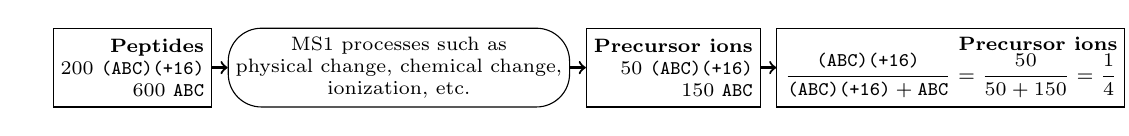
\begin{tikzpicture}
\scriptsize
\tikzset{
	rblock/.style={draw, shape=rectangle,                      align=right, minimum width=1cm,minimum height=1cm},
	block/.style= {draw, shape=rectangle,rounded corners=1.5em,align=center,minimum width=3cm,minimum height=1cm},
	lblock/.style={draw, shape=rectangle,                      align=center,minimum width=3.5cm,minimum height=1cm},
}
\node[rblock](1st){
	\bf{Peptides} \\ 
	200 \texttt{(ABC)(+16)} \\
	600 \texttt{ABC}
};
\node[block,right=.2cm of 1st](cid){
	\Gls{MS1} processes such as \\ physical change, chemical change, \\ ionization, etc.
};	
\node[rblock, right=.2cm of cid](2nd){
	\bf{Precursor ions}     \\     
	50  \texttt{(ABC)(+16)} \\
	150 \texttt{ABC}
	};
\node[rblock, right=.2cm of 2nd](3rd){
	\bf{Precursor ions}\\
	\( \displaystyle\frac{\texttt{{(ABC)(+16)}}}{{\texttt{(ABC)(+16)} + \texttt{ABC}}} = \frac{50} {50+150}  = \frac{1}{4} \)
};
\path[draw,->, thick] (1st) edge (cid)  (cid) edge (2nd)  (2nd) edge (3rd);
\end{tikzpicture}
\\ {} \\\noindent
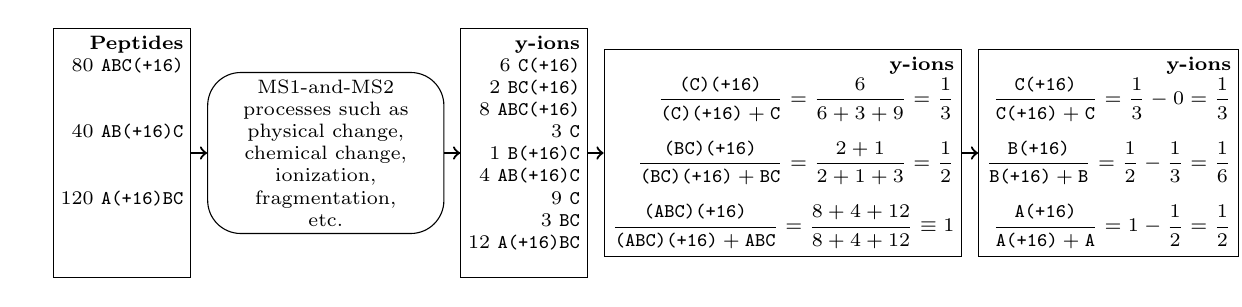
\begin{tikzpicture} %[>=latex']
	\scriptsize
	\tikzset{
		rblock/.style={draw, shape=rectangle,                      align=right, minimum width=1cm,minimum height=1cm},
		block/.style= {draw, shape=rectangle,rounded corners=1.5em,align=center,minimum width=3cm,minimum height=1cm},
		lblock/.style={draw, shape=rectangle,                      align=center,minimum width=3.5cm,minimum height=1cm},
	}
	\node[rblock](1st){
		\bf{Peptides} \\ 
		80  \texttt{ABC(+16)}\\~\\~\\
		40  \texttt{AB(+16)C}\\~\\~\\
		120 \texttt{A(+16)BC}\\~\\~\\
	};
	\node[block,right=.2cm of 1st](cid){
		\gls{MS1}-and-\gls{MS2} \\ processes such as \\ physical change, \\ chemical change, \\ ionization, \\ fragmentation, \\ etc.
	};
	\node[rblock, right=.2cm of cid](2nd){
		\bf{y-ions}     \\     
		6  \texttt{C(+16)} \\ 2 \texttt{BC(+16)}  \\8  \texttt{ABC(+16)} \\
		3  \texttt{C}      \\ 1 \texttt{B(+16)C}  \\4  \texttt{AB(+16)C} \\
		9  \texttt{C}      \\ 3 \texttt{BC}       \\12 \texttt{A(+16)BC} \\
		};
	\node[rblock, right=.2cm of 2nd](3rd){
		\bf{y-ions}\\
		\( \displaystyle\frac{\texttt{(C)(+16)}}{\texttt{(C)(+16)}+\texttt{C}}    = \frac{6}     {6+3+9}  = \frac{1}{3} \) \\ \vspace{4pt} \\
		\( \displaystyle\frac{\texttt{(BC)(+16)}}{\texttt{(BC)(+16)}+\texttt{BC}} = \frac{2+1}   {2+1+3}  = \frac{1}{2} \) \\ \vspace{4pt} \\
		\( \displaystyle\frac{\texttt{(ABC)(+16)}}{\texttt{(ABC)(+16)}+\texttt{ABC}} = \frac{8+4+12}{8+4+12} \equiv 1 \)
	};
	\node[rblock, right=.2cm of 3rd](4th){
		\bf{y-ions}\\
		\( \displaystyle\frac{\texttt{C(+16)}}{\texttt{C(+16)}+\texttt{C}} = \frac{1}{3} - 0           = \frac{1}{3} \) \\ \vspace{4pt} \\
		\( \displaystyle\frac{\texttt{B(+16)}}{\texttt{B(+16)}+\texttt{B}} = \frac{1}{2} - \frac{1}{3} = \frac{1}{6} \) \\ \vspace{4pt} \\
		\( \displaystyle\frac{\texttt{A(+16)}}{\texttt{A(+16)}+\texttt{A}} = 1           - \frac{1}{2} = \frac{1}{2} \) 
	};
	\path[draw,->, thick] (1st) edge (cid)  (cid) edge (2nd)  (2nd) edge (3rd) (3rd) edge (4th);
\end{tikzpicture}
\noindent
\footnotesize{
\noindent
\begin{align*}
	    \displaystyle\Pr[\mathtt{C_{}} \text{ is } \gls{mono-oxidized}] = \frac{1}{4} \cdot \frac{1}{3} %= \frac{1}{12}  
	&&  \displaystyle\Pr[\mathtt{B_{}} \text{ is } \gls{mono-oxidized}] = \frac{1}{4} \cdot \frac{1}{6} %= \frac{1}{24}   
	&&  \displaystyle\Pr[\mathtt{A_{}} \text{ is } \gls{mono-oxidized}] = \frac{1}{4} \cdot \frac{1}{2} %= \frac{1}{8}   
\end{align*}
\noindent
Our algorithm quantitates \gls{ox1} at subpeptide level on a dataset produced by targeted \gls{LC-MS/MS}. 
	This quantitation can improve the spatial resolution of \gls{RP-MS}.
  This improvement improves the spatial resolution at which protein folding is studied.
}	
\endgroup
\end{framed}
\caption[
	The graphical abstract of \cref{chap:oxlvl}.]{
	The graphical abstract of \cref{chap:oxlvl} (hypothetical data used as example).
	\label{fig:OX:motivation:graphical-abstract}}
\end{figure}
\clearpage

%This chapter present our work on the quantitation of oxidation at subpeptide level.
\Cref{sec:subpeptide-oxidation:motivation} presents our motivation.
Our motivation is to improve the spatial resolution of \gls{RP-MS},
	because this improvement improves the spatial resolution at which protein folding is studied.
\Cref{sec:oxlvl:relatedworks} presents related works in the literature. 
\Cref{sec:oxlvl:dataset} presents an \gls{MS/MS} dataset produced by a variant of \gls{RP-MS}.
The \gls{MS/MS} dataset is mainly produced by six runs of targeted \gls{MS/MS} respectively analyzing six \gls{mono-oxidized} tryptic peptides. 
\Cref{sec:oxlvl:methods} presents our algorithm.
Our algorithm takes as input the data produced by a run of targeted \gls{MS/MS},
	and our algorithm quantitates the oxidation on a subpeptide of the peptide analyzed by this run.
\Cref{sec:oxlvl:results} presents the results of running our algorithm on the \gls{MS/MS} dataset. 
These results are collectively consistent with some previously published oxidation rates.
\Cref{sec:oxlvl:discussion} presents the discussion about our work.
	
\section{Motivation}
\label{sec:subpeptide-oxidation:motivation}

%Let proteolyzed peptides be the products of the proteolysis of a polypeptide.
The proteolysis of a polypeptide produces some proteolyzed peptides.	
Quantitating oxidation at peptide level    means quantitating the extent of oxidation on a proteolyzed peptide.
Quantitating oxidation at subpeptide level means quantitating the extent of oxidation on a short peptide that is part of a proteolyzed peptide.
Quantitating oxidation at residue level    means quantitating the extent of oxidation on one single residue of a proteolyzed peptide. 
		
We proposed an algorithm for quantitating, at subpeptide level, the \gls{ox1} produced by \gls{FPOP} and detected by targeted \gls{LC-MS/MS}.
%Our algorithm empirically works on a dataset that is generated by an \gls{RP-MS} experiment with six runs of targeted product-ion scans.
Our algorithm can improve the spatial resolution of \gls{RP-MS}.
This improvement can improve the spatial resolution at which \gls{RP-MS} is used for studying protein folding.
Moreover, our work is an important step towards quantitation of oxidation at residue level.

\section{Related works}
\label{sec:oxlvl:relatedworks}

In \citeyear{maleknia1999millisecond}, \citet{maleknia1999millisecond} used Synchrotron X-rays to generate \gls{OH-rad} within 10 milliseconds. 
In \citeyear{maleknia1999millisecond}, \citet{maleknia1999electrospray} used electrical discharge to oxidize proteins that are introduced into a mass spectrometer.
Since then, many analytical methods for generating \gls{OH-rad} have been developed.
Unfortunately, these methods suffer from the uncertainty that \gls{OH-rad} can partially denature an investigated protein.
Moreover, these methods cannot efficiently control the extent of \gls{OH-rad}-mediated modification to an investigated protein.

In \citeyear{hambly2005laser}, \citet{hambly2005laser} developed \gls{FPOP}.
\Gls{FPOP} reduces the chemical effect of \gls{OH-rad} to less than 1 microsecond.
Moreover, \gls{FPOP} limits the extent of \gls{OH-rad}-mediated modifications by using a radical scavenger, such as glutamine.
Since then, \gls{FPOP} has been extensively used for \gls{RP-MS}.
Unfortunately, \gls{RP-MS} has only been used to quantitate oxidation at peptide level.
Different amino acids respectively have hugely different rates of reaction with \gls{OH-rad} (\cref{tab:AA-OH-reaction-rate}). %TODO: clarity?
Thus, if the rate of such reaction of an amino-acid residue is negligible, then this residue is often assumed to be always unoxidized.

Some methods were proposed to quantitate oxidation at subpeptide level.
In \citeyear{chen2012fast},
	\citet{chen2012fast} used \gls{MS2} spectra to map some peaks in \gls{MS1} spectra to some oxidized residues, 
	then \citet{chen2012fast} used this mapping to quantitate the oxidation on each of some selected residues of Barstar. 
Unfortunately, this mapping requires considerable human effort, and this quantitation requires a high-resolution mass spectrometer.
Moreover, this mapping is often compromised by the overlap between the respective \glspl{RT} of differently oxidized isobaric peptides.
In \citeyear{li2013improved}, \citet{li2013improved} used c-ion intensities to quantitate, with some errors, oxidation at subpeptide level.
Unfortunately, \citet{li2013improved} did not discuss about the correction of these errors and investigated only two real peptides.

\section{The \texorpdfstring{\Gls{MS/MS}}{MS/MS} dataset}
\label{DS:MS2}
\label{sec:oxlvl:dataset}

\begin{figure}
\def \noCommand #1{#1}
\centering{\texttt{
	\begin{tabular}{l}
		\noCommand{>\texttt{1WLA:A}|PDBID|CHAIN|SEQUENCE} \\
		\underline{GLSDGEWQQVLNVWGK} %$^\texttt{1814.90}$ 
		\underline{VEADIAGHGQEVLIR} %$^\texttt{1605.85}$  
		\underline{LFTGHPETLEK} %$^\texttt{1270.66}$  
		\noCommand{FDK} \\
		\noCommand{FKHLK} 
		\underline{TEAEMK} %$^\texttt{707.32}$   
		\noCommand{ASEDLK} 
		\noCommand{K} %\\
		\noCommand{HGTVVLTALGGILK} 
		\noCommand{K} 
		\noCommand{K} 
		\noCommand{GHHEAELKPLAQSHATKHK} \\
		\noCommand{IPIKYLEFISDAIIHVLHSK}  
		\underline{HPGDFGADAQGAMTK} %$^\texttt{1501.66}$  
		\noCommand{ALELFR} 
		\noCommand{NDIAAK}
		\noCommand{YK} 
		\underline{ELGFQG} %$^\texttt{649.31}$ 
	\end{tabular}
}}
\caption[
	The FASTA sequence of apomyoglobin (\gls{PDB} \texttt{1WLA:A}).]{
	The FASTA sequence of apomyoglobin (\gls{PDB} \texttt{1WLA:A}).
	Each word denotes a tryptic peptide.
	All tryptic peptides are analyzed in one run of \gls{MS1}.{}
	However, 
	only the six underlined tryptic peptides are analyzed in six runs of targeted \gls{MS2} respectively. 
 	\label{FASTA_PDB_1WLA}}
\end{figure}

The \gls{MS/MS} dataset is produced by an \gls{RP-MS} experiment.
This experiment is conducted by Siavash Vahidi and Professor Lars Konermann.
This experiment is similar to the other experiment described in \cite{vahidi2012mapping}.
This experiment proceeded as follows.
First, a solution with pH=2 denatured apomyoglobin (\gls{PDB} \texttt{1WLA:A}).
Next, \gls{FPOP} oxidized most of this denatured apomyoglobin, although most tryptic peptides of apomyoglobin remain unoxidized.
Then, trypsin cleaved oxidized apomyoglobin into tryptic peptides.
Each of these tryptic peptides was either oxidized or unoxidized.
Afterwards, one run of \gls{LC-MS} analyzed these tryptic peptides to produce a sequence of \gls{MS1} spectra.
Finally, six runs of targeted \gls{LC-MS/MS} respectively analyzed six \gls{mono-oxidized} tryptic peptides among these peptides.
Each of these six runs produced a sequence of \gls{MS2} spectra.
\Cref{FASTA_PDB_1WLA} shows the sequence of apomyoglobin and the six \gls{mono-oxidized} tryptic peptides.
The \gls{FPOP} presumably used a finely tuned quantity of radical scavengers to control oxidation extents.
Thus, the sequence of \gls{MS1} spectra shows that a tryptic peptide of apomyoglobin is rarely oxidized more than once.
Thus, any tryptic peptide of apomyoglobin is assumed to be either unoxidized or \gls{mono-oxidized} after the \gls{FPOP}.
\begin{table}
%	\def \textst #1{{\texttt{#1}}}
%	\def \txtfrac #1#2{\(\genfrac{}{}{0pt}{}{\displaystyle\text{#1}}{\displaystyle\text{#2}}\)}
%	\def \ss #1#2{\(\substack{\displaystyle\text{#1}\\\displaystyle\text{#2}}\)}
%	\def \sss #1#2#3{\(\substack{\displaystyle\text{#1}\\\displaystyle\text{#2}\\\displaystyle\text{#3}}\)}
%	\def \M #1{\textnormal{M}}
  \centering\small
  \begin{tabular}{ l c c c c c c c c c c}
  \toprule
  Sequence of both  
                                &\multicolumn{4}{l}{For precursor ions of \gls{typeof:ox=1:pep}}  
                                &\multicolumn{4}{l}{For precursor ions of \gls{typeof:ox=0:pep}}  \\      
  \gls{typeof:ox=1:pep} and \gls{typeof:ox=0:pep}    
                                & \gls{RT} in min    & z         & \gls{m/z}    & \gls{AUCXIC}  
                                & \gls{RT} in min    & z         & \gls{m/z}    & \gls{AUCXIC} 
                                \\\midrule
  \texttt{GLSDGEWQQVLNVWGK}     & [49.0, 62.0]   & 3         & 611.30 & 12377 & [59.0, 64.0] & 3 & 605.97 &  17390 \\
  \texttt{VEADIAGHGQEVLIR}      & [28.3, 40.3]   & 3         & 541.62 & 29232 & [34.0, 83.0] & 3 & 536.29 & 249193 \\
  \texttt{LFTGHPETLEK}          & [22.5, 34.0]   & 3         & 429.89 & 24164 & [28.5, 37.0] & 3 & 424.56 & 123514 \\
  \texttt{TEAEMK}               &  [0.0, 7.0]    & 2         & 362.66 &  4545 & [10.0, 14.8] & 2 & 354.67 &  14512 \\
  \texttt{HPGDFGADAQGAMTK}      & [19.5, 27.0]   & 3         & 506.89 & 20141 & [26.7, 33.3] & 3 & 501.56 &   6005 \\
  \texttt{ELGFQG}               & [21.0, 34.0]   & 1         & 666.31 &  9365 & [31.9, 37.9] & 1 & 650.32 &  81906 \\
  \bottomrule
  \end{tabular}
  \caption[A summary of the \gls{MS1} spectra in the \gls{MS/MS} dataset.]{
           A summary of the \gls{MS1} spectra in the \gls{MS/MS} dataset.
  The \gls{m/z} window that is used for constructing \glspl{XIC} and thus \glspl{AUCXIC} is the \gls{m/z} of the precursor ion \(\pm 0.1\si{\dalton}\).
  	The \gls{AUCXIC} of all multiply-oxidized (e.g. di-oxidized, tri-oxidized) peptides is at most 10\% of the \gls{AUCXIC} of the corresponding \gls{mono-oxidized} peptide (data not shown).
	\Gls{typeof:ox=0:pep} is a chemical species of unoxidized peptides.{}
  \Gls{typeof:ox=1:pep} is a chemical superspecies of \gls{mono-oxidized} peptides that are chemically identical up to \gls{ox1}-induced structural isomerism.
  \label{tab:oxlvl:6-tryptic-peptides}
  }
\end{table}
We manually verified, by visual inspection, that the mass spectrometer that produced the \gls{MS/MS} dataset has a mass accuracy of \(\pm0.1\si{\dalton}\).
Peptides having the same sequence respectively generate precursor ions having the same charge state (\cref{tab:oxlvl:6-tryptic-peptides}). 

In this section,
	\gls{typeof:ox=0:pep} \glsentryuseri{typeof:ox=0:pep},
	and \gls{typeof:ox=1:pep} \glsentryuseri{typeof:ox=1:pep}.
\Gls{AUCXIC} \glsdesc*{AUCXIC} % lower-case to denote function

\section{Methods}
%\label{sec:OX:methods}
\label{sec:oxlvl:methods}

In brief, our algorithm proceeds as follows.
First, oxidation at peptide level is quantitated by using \gls{MS1} spectra.
Next, oxidation at subpeptide level is quantitated by using \gls{MS2} spectra.
Then, random errors in the quantitation of oxidation at subpeptide level are estimated by our empirical formula presented in \cref{chap:error},
Afterwards, every such quantitated extent of oxidation is ensured to be a positive number.
Finally, by using both quantitation of oxidation at subpeptide level and quantitation of oxidation at peptide level,
	our algorithm quantitates oxidation at subpeptide level for multiple peptides in a protein.
The input mass spectra had first been preprocessed by PEAKS 6 \cite{ma2003peaks} before being used by our algorithm.				

Every y-ion is indexed from C-terminus to N-terminus, but every residue is indexed from N-terminus to C-terminus (\cref{MS2_pept_id}).
Thus, an index such as \(i\) is a y-ion index if used for indexing a y-ion and a residue index if used for indexing a residue.

\begin{figure}
\includegraphics[width=\textwidth]{imgbin/oxidPeakArea.pdf}
\caption[
	A schematic of \gls{MS1}-based quantitation of oxidation at peptide level.]{
	A schematic of \gls{MS1}-based quantitation of oxidation at peptide level.
	A hypothetical run is used as example.
	The \gls{mono-oxidized} forms can be chemically different and thus can be eluted at different \gls{RT} ranges respectively.
	\label{fig:OX:methods:quntitationMS1}
}
\end{figure}	
Before quantitating oxidation at subpeptide level, we have to quantitate oxidation at peptide level.
In \gls{MS1} spectra, 
	the fraction of the \gls{AUCXIC} of \gls{mono-oxidized} peptide over the \gls{AUCXIC} of both \gls{mono-oxidized} or unoxidized peptide denotes the relative frequency that this peptide is oxidized after \gls{FPOP}.
Thus, this \gls{AUCXIC} fraction is used for quantitating oxidation at peptide level.
\Cref{fig:OX:methods:quntitationMS1} shows how \gls{MS1} enables the quantitation of oxidation at peptide level.
	
In the \gls{LC-MS/MS} experiment, the instrument is programmed to target a \gls{mono-oxidized} peptide \gls{typeof:ox=1:pep}. 
When \gls{typeof:ox=1:pep} is eluted from \gls{LC} column, \gls{typeof:ox=1:pep} is continuously acquired by the mass spectrometer and fragmented. 
The product ions of \gls{typeof:ox=1:pep} are detected to produce an \gls{MS2} spectrum. 
As a result, a sequence of \gls{MS2} spectra are produced. 
For any index \(i\), we use \(\texttt{y}_i\oxZero\) to denote the unoxidized \(\texttt{y}_i\) ion and \(\texttt{y}_i'\) to denote the \gls{mono-oxidized} \(\texttt{y}_i\) ion. 
The \gls{AUCXIC} of \(\texttt{y}_i\oxZero\) or \(\texttt{y}_i'\) is the total intensities of the corresponding ion in the sequence of \gls{MS2} spectra, and is denoted by \(y_i\oxZero\) or \(y_i'\), respectively. 
Thus, \(\phi_i\), the fraction of \(\texttt{y}_i\) ions that are \gls{mono-oxidized}, can be estimated by the following formula.
\(\displaystyle \phi_i \getsvalueof \frac{y_i'}{y_i+y_i'}\).	
	
Because of the stochastic nature of every run of mass spectrometry and of the algorithmic artifact in the calculation of \gls{AUCXIC},
	random error exists in the observation of \(\phi_i\).
One run of mass spectrometry cannot empirically assess any random error.
Fortunately, \cref{chap:error} provides an empirical formula that estimates the following: 
	the random error in a \gls{AUCXIC} fraction given that this fraction is measured in only one run of mass spectrometry.
Thus, we applied our empirical formula to \(\phi_i\), because \(\phi_i\) is a \gls{AUCXIC} fraction.
The substitution of \(\phi_i\) into our empirical formula implies that
\begin{align}
\displaystyle\Phi_i \isappdistas \rnorm\left({\E}[\Phi_i], \frac{y_i{\oxZero} \cdot y_i'}{(y_i{\oxZero} + y_i')^{3}}\right),
\label{eq:OX:methods:empirical_formula}
\end{align}
where \(\phi_i\) is one realization, or equivalently one observed value, of the hidden random variable \(\Phi_i\).
\(\Phi_i\) denotes the hidden stochastic process that generated \(\phi_i\) with random error.
\(\phi_i\) is trivially an estimate of \({\E}[\Phi_i]\).
Thus, let \({\singlehat\E}[\Phi_i]\) be defined as \(\phi_i\).
	

The quantity of every y-ion should be proportional to the quantity of the peptides that can generate this y-ion.
Thus, \( y_i'\) should be proportional to the quantity of \gls{mono-oxidized} peptides whose \gls{ox1} site is before or at the y-ion index \(i\). 
Similarly, \( y_i{\oxZero}\) should be proportional to the quantity of \gls{mono-oxidized} peptides whose \gls{ox1} site is after the y-ion index \(i\).
Thus, by definition, \({\singlehat\E}[\Phi_i]\) denotes the relative frequency that the oxidation site on \(\gls{typeof:ox=1:pep}\) is before or at the y-ion index \(i\).
Thus, \(\displaystyle {\singlehat\E}[\Phi_i] - {\singlehat\E}[\Phi_{i-1}]\) denotes the relative frequency that the oxidation site on \(\gls{typeof:ox=1:pep}\) is at the y-ion index \(i\).

Relative frequency cannot be negative.
Thus, for every applicable \(i\), \({\singlehat\E}[\Phi_i] - {\singlehat\E}[\Phi_{i-1}]\) should be positive.
Equivalently, \(\displaystyle {\singlehat\E}[\Phi_i]\) should monotonically increase as a function of \(i\).
For example, this monotonicity almost holds for \texttt{(VEADIAGHGQEVLIR)(+16)} (\cref{fig:OX:dataset:oxid_vs_unox_for_VEADIAGHGQEVLIR}).
\begin{figure}
\includegraphics[width=\textwidth]{img/VEADIAGHGQEVLIR_34_68_ox0.pdf}
\includegraphics[width=\textwidth]{img/VEADIAGHGQEVLIR_34_68_ox1.pdf}
\caption[
	A mixture \gls{MS2} spectrum of \texttt{VEADIAGHGQEVLIR} in the \gls{MS/MS} dataset.]{
	A mixture \gls{MS2} spectrum of \texttt{VEADIAGHGQEVLIR} in the \gls{MS/MS} dataset.
	The top annotation shows \(\texttt{y}_i\) and the bottom annotation shows \(\texttt{y}_i'\).
	\(i\) denotes an y-ion index. 
	\(\texttt{y}\) denotes the unoxidized form of a y-ion. 
	\(\texttt{y}'\) denotes the \gls{mono-oxidized} forms of a y-ion.
	Both annotations annotate the same spectrum.
	\label{fig:OX:dataset:oxid_vs_unox_for_VEADIAGHGQEVLIR}
}
\end{figure}	
This monotonicity is desired but not observed for some pairs of y-ion indexes.
This monotonicity can be invalidated by multiple causes.
However, the most important cause among these causes seems to be the stochastic nature of \(\Phi_i\) that generated \(\phi_i\).
This stochastic nature causes random error in the observation of \(\phi_i\).
An estimation of this random error is provided by \cref{eq:OX:methods:empirical_formula}.
Then, by considering this random error, \cref{alg:OX:methods:plot:generate_subpeptide_level_oxidation} of \cref{alg_get_2plots} enforces this monotonicity.		

The z-score of an observation is defined as follows: 
	the deviation of this observation from the mean of this observation, divided by the standard deviation of this observation.
%Z-score is defined as observed deviation from mean divided by standard deviation.
The standard deviation of \(\Phi_i\) can be estimated by \cref{eq:OX:methods:empirical_formula}.
Thus, \cref{eq:OX:methods:empirical_formula} can normalize observed deviations respectively to z-scores.
Thus, the sum of the respective squares of these z-scores monotonically decreases as a function of the likelihood of observing these z-scores.
This monotonic decrease leads to isotonic regression.
Thus, the exact formulation of our isotonic regression is as follows given the length \(n\) of the sequence of a peptide:
\begin{align}   
&\text{Minimize }  &&
		\sum_{i=1}^{n-1} \left(\frac{{\doublehat\E}[\Phi_i] - {\singlehat\E}(\Phi_i)}{\sqrt{{\singlehat\VAR}(\Phi_i)}}\right)^2 \\
&\text{such that } &&
		\forall i\in\{2,3,\dots,n-1\}: \left(0 \le {\doublehat\E}[\Phi_{i-1}] \le {\doublehat\E}[\Phi_{i}] \le 1\right) \\
&\text{where }     &&
		\displaystyle{\singlehat\E}(\Phi_i) = \phi_i = \frac{y_i'}{y_i\oxZero + y_i{'}} 
		\text{~~~~and~~~~} \displaystyle{\singlehat\VAR}(\Phi_i) = \frac{y_i{\oxZero} + y_i'}{(y_i{\oxZero} \cdot y_i')^{3}}.
\end{align}  		
Our isotonic regression is solved by using the linear-time pool-adjacent-violators algorithm (PAVA) implemented by \citet{turner2013package}.

The solution to our isotonic regression transforms each \({\singlehat\E}[\Phi_i]\) into its corresponding	\({\doublehat\E}[\Phi_i]\).
By definition of isotonic regression,
	\({\doublehat\E}[\Phi_{i}] - {\doublehat\E}[\Phi_{i-1}] \ge 0\) for all valid y-ion indexes \(i\) and \(i+1\).
Thus, every \({\doublehat\E}[\Phi_{i}] - {\doublehat\E}[\Phi_{i-1}]\) can denote a valid relative frequency.
	%and a valid quantity of molecular entities.
Thus, \({\doublehat\E}[\Phi_{i}] - {\doublehat\E}[\Phi_{i-1}]\) denotes the relative frequency of the following event: 
	the residue located at the y-ion index \(i\) of a peptide is \gls{mono-oxidized} given that this peptide as a whole is \gls{mono-oxidized}.
The random error in each \({\singlehat\E}[\Phi_{i}]\) is estimated to be approximately \(\sqrt{{\singlehat\VAR}[\Phi_i]}\),
	and \({\singlehat\E}[\Phi_{i}] \approx {\doublehat\E}[\Phi_{i}]\).
Thus, the random error in \({\doublehat\E}[\Phi_{i}]\) is also estimated to be approximately \(\sqrt{{\singlehat\VAR}[\Phi_i]}\).
Thus, if \(\Phi_i\) and \(\Phi_{i-1}\) are independent,
	then the random error in \({\singlehat\E}[\Phi_{i} - \Phi_{i-1}]\) is estimated to be approximately \(\sqrt{{\singlehat\VAR}[\Phi_{i}] + {\singlehat\VAR}[\Phi_{i-1}]}\).{}
Thus,
	the random error in the observed \({\doublehat\E}[\Phi_{i}] - {\doublehat\E}[\Phi_{i-1}]\) is estimated to be approximately
		\(\sqrt{{\singlehat\VAR}[\Phi_{i}] + {\singlehat\VAR}[\Phi_{i-1}]}\).

We can quantitate both the \gls{ox1} on each peptide and the \gls{ox1} on each residue of a \gls{mono-oxidized} peptide.
Thus, we can quantitate the \gls{ox1} on each residue.
\Cref{alg:OX:methods:plot:generate_subpeptide_level_oxidation} of \cref{alg_get_2plots} 
		calculates \gls{ox1} at residue level by using this quantitation. 
%\gls{ox1} at peptide level and \gls{ox1} at residue level given \gls{ox1} at peptide level.
Afterwards, the relative frequency that each residue is \gls{mono-oxidized} is estimated.
Finally, the random error in this relative frequency is estimated too. 

Some errors exist in our \gls{MS1}-based quantitation of oxidation at peptide level.
However, a peptide can be divided into multiple subpeptides.
Thus, the extent of oxidation on each of these subpeptide is only a small difference between two \gls{AUCXIC} fractions.
Thus, quantitation of oxidation at subpeptide level has more error than quantitation of oxidation at peptide level.
Moreover, the intensity of a product ion is usually much lower than the intensity of the precursor ion that formed this product ion.
Thus, \gls{MS2}-based quantitation of oxidation has more error than \gls{MS1}-based quantitation of oxidation.
We used both such \gls{MS2}-based quantitation at subpeptide level and such \gls{MS1}-based quantitation at peptide level.
Therefore, we ignored error in such \gls{MS1}-based quantitation because such \gls{MS2}-based quantitation has much more error.

As mentioned in \cref{sec:MS:prep}, preprocessing of mass spectra is important.
Examples of such preprocessing are baseline removal, centroiding, deconvolution, and deisotoping.
Thus,	before applying any aforementioned procedure, we performed the following.
First, we manually determined the charge state of every applicable precursor. 
Then, we performed a moving average with a window of \(20\si{\second}\) along \gls{RT} for the \gls{MS2} spectra in the \gls{MS/MS} dataset.
Finally, we let the software PEAKS 6 \cite{ma2003peaks} preprocess these \gls{MS2} spectra.	

\begin{algorithm}
	\def \Moxid {\ensuremath{P'}}
	\def \Munox {\ensuremath{P{\oxZero}}}
		\def \Moxid {\gls{typeof:ox=1:pep}}
		\def \Munox {\gls{typeof:ox=0:pep}}
	\def \DIAMS {\ensuremath{r''}}
	\def \PREMS {\ensuremath{r'}}
\caption{
	quantitate-oxidation-at-subpeptide-level\((\Munox, \Moxid, r', r'')\) 
	\label{alg_get_2plots}}
\begin{algorithmic}[1]	
\Require{
	\(\Munox\) is a chemical species of unoxidized peptides.
	\(\Moxid\) is a chemical superspecies of \gls{mono-oxidized} peptides.
	Both \(\Munox\) and \(\Moxid\) have the same sequence and \(\Moxid\) is heavier than \(\Munox\) by approximately \(15.99\si{\dalton}\).
	A sample contains both \(\Munox\) and \(\Moxid\). 
	A run of \gls{LC-MS} surveyed this entire sample to produce a sequence \(\PREMS\) of \gls{MS1} spectra.
	A run of \gls{LC-MS/MS} targeted only \(\Moxid\) in this sample to produce a sequence \(\DIAMS{}\) of \gls{MS2} spectra.
}
\Ensure{
		\Cref{plot_yratio_vs_i} and
		\cref{plot_ox_vs_pepidx}.
	}
	\State \(\displaystyle {\singlehat\Pr}[\Munox\to\Moxid]\isdefinedas\frac{\gls{AUCXIC}(\Moxid, r')}{\gls{AUCXIC}(\Moxid, r') + \gls{AUCXIC}(\Munox,  r')}\) 
	\newline\Comment{quantitate \gls{ox1} at peptide level by using information in \gls{MS1}}
	\State Smooth \DIAMS{} by a moving average of 20 \gls{MS2} spectra that are consecutive along \gls{RT}.  \newline
	\Comment{Numbers other than 20 yield similar results.}
	\State Preprocess smoothed \DIAMS{} using PEAKS 6 \cite{ma2003peaks}.
	\State \(n \isdefinedas\) the length of the sequence of \(\Munox\) or equivalently of \(\Moxid\).
	\For{\(i\in \{1,2,\dots,n{-}1\}\)}
		\State \( y_i{\oxZero} \isdefinedas \gls{AUCXIC}(\texttt{y}_i{\oxZero}(\Moxid), r'') + i \)  
		\State \( y_i' \isdefinedas \gls{AUCXIC}(\texttt{y}_i'(\Moxid), r'') + (n-i) \)  
		\State \(\displaystyle ({\singlehat\E}[\Phi_i], {\singlehat\VAR}[\Phi_i]) 
				\isdefinedas \left(\frac{y_i'}{y_i{\oxZero}+y_i'},
				                  \frac{{y_i{\oxZero}}\cdot y_i'}{(y_i{\oxZero}+y_i')^3}\right)\) 
				\hfill\Comment{\Cref{eq:NM:derivation:simplificationresult}}
	\EndFor
	\State Plot \({\singlehat\E}[\Phi_i] \pm \sqrt{{\singlehat\VAR}[\Phi_i]}\) as a function of \(i\),
			and this plot is in \cref{plot_yratio_vs_i}. 
	\State \(\displaystyle
	({\doublehat\E}[\Phi_1], {\doublehat\E}[\Phi_2], \dots, {\doublehat\E}[\Phi_{n-1}])  \getsvalueof 
	\argmin_{ \substack{ (\phi_1, \phi_2, \dots, \phi_{n-1}) \in [0,1]^{n-1} \\ 
	                     \text{ such that } \phi_1 \le \phi_2 \le \dots \le \phi_{n-1} }}
	\left(
		\sum_{i=1}^{n-1} \left(\frac{\phi_i - {\singlehat\E}(\Phi_i)}{\sqrt{{\singlehat\VAR}(\Phi_i)}}\right)^2 
	\right) \)
	\newline
	\Comment{Perform isotonic regression of \({\singlehat\E}[\Phi_i]\) versus \(i\) where each \({\singlehat\E}[\Phi_i]\) has weight \(({\singlehat\VAR}[\Phi_i])^{-1}\)}\newline
	\Comment{The PAVA implemented by \citet{turner2013package} is used for solving our isotonic regression.}
	\State \((({\singlehat\E}[\Phi_0], {\singlehat\VAR}[\Phi_0]), ({\singlehat\E}[\Phi_n], {\singlehat\VAR}[\Phi_n])) 
			\getsvalueof ((0, 0), (1, 0)) \) \hfill \Comment{Oxidation before \(0\) and \(n\)}  
	\For{\(i \in \{1,2,\dots, n\}\)}
		\State \(\displaystyle 
				\left(
					{\doublehat\E}[\Phi_i - \Phi_{i-1}],
					{\doublehat\VAR}[\Phi_i - \Phi_{i-1}]
				\right) 
				\isdefinedas 
				\left(
					{\doublehat\E}[\Phi_i] - {\doublehat\E}[\Phi_{i-1}], 
					{\singlehat\VAR}[\Phi_{i}] + {\singlehat\VAR}[\Phi_{i-1}]
					%\sum_{j=i-1}^{i} \left(({\doublehat\E}[\Phi_j] - {\singlehat\E}[\Phi_j])^2 + {\singlehat\VAR}[\Phi_{j}]\right)
				\right)
			\)
			\State \({\singlehat\Pr}[\Munox_{n+1-i}\to\Moxid_{n+1-i}] \isappdistas 
		    {\singlehat\Pr}[\Munox\to\Moxid] \cdot \rnorm\left(
								{\doublehat\E}[\Phi_i - \Phi_{i-1}],
								{\doublehat\VAR}[\Phi_i - \Phi_{i-1}]
							\right)\)
				\label{alg:OX:methods:plot:generate_subpeptide_level_oxidation}
	\EndFor
	\State Plot \({\singlehat\Pr}[\Munox_{k}\to\Moxid_{k}]\) as a function of the residue at index \(k\) of \(\Munox{}\) or equivalently of \(\Moxid{}\), 
			{and this plot is in \cref{plot_ox_vs_pepidx}}. 
			
\end{algorithmic}
\end{algorithm}


\section{Results on the \texorpdfstring{\gls{MS/MS}}{MS/MS} dataset}
\label{sec:oxlvl:results}

\begin{figure}
\begin{center}
\begin{tikzpicture}
\begin{axis}[
 ticks=none,enlargelimits=false,
		xlabel near ticks, ylabel near ticks, 
		width=\textwidth,height=\textwidth,
		ylabel={\({\singlehat\E}(\Phi_i) \pm {\singlehat\VAR}(\Phi_i)\) fitted with isotonic regression},
		xlabel={y-ion index (\(i\))}]
  \addplot graphics[xmin=0,xmax=100,ymin=0,ymax=100] {plt/1_pep_ratio_all.pdf};
\end{axis}
\end{tikzpicture}
\end{center}
\caption[ % $...$ instead of \(...\) should be used here
	The estimated relative frequency that $\texttt{y}_i$ is \gls{mono-oxidized} as a function of $i$.]{
	The estimated relative frequency that $\texttt{y}_i$ is \gls{mono-oxidized} as a function of $i$.
	\Cref{alg_get_2plots} generated this plot.
	\label{plot_yratio_vs_i}}
\end{figure}

\Cref{alg_get_2plots} generated \cref{plot_yratio_vs_i} from the \gls{MS/MS} dataset which is described in \cref{DS:MS2}. 
As mentioned in \cref{sec:oxlvl:methods}, the expected pattern is that \(\Phi_i\) does not substantially decrease as the y-ion index \(i\) increases.
\Cref{plot_yratio_vs_i} shows the following.
The \gls{mono-oxidized} forms of \texttt{GLSDGEWQQVLNVWGK} show the expected pattern at all y-ion indexes without any exception. 
The \gls{mono-oxidized} forms of \texttt{VEADIAGHGQEVLIR}  show the expected pattern at all y-ion indexes except from \(i=9\) to \(i=10\).
The \gls{mono-oxidized} forms of \texttt{LFTGHPETLEK}      show the expected pattern at all y-ion indexes except from \(i=5\) to \(i=6\) and from \(i=8\) to \(i=9\).
The \gls{mono-oxidized} forms of \texttt{TEAEMK}           show the expected pattern at all y-ion indexes except from \(i=2\) to \(i=3\) and from \(i=4\) to \(i=5\).
The \gls{mono-oxidized} forms of \texttt{HPGDFGADAQGAMTK}  show the expected pattern at all y-ion indexes except from \(i=5\) to \(i=6\).
The \gls{mono-oxidized} forms of \texttt{ELGFQG}           show the expected pattern at all y-ion indexes without any exception.

The native reactivity of a free amino acid with \gls{OH-rad} is positively correlated with the percentage of \gls{ox1} on this residue. 
%detected as mass shift of \(+15.99\si{\dalton}\) on this residue.
%This correlation should be strongly linear.
Unfortunately, this correlation is weak mainly because of the following.
The reaction of a residue with \gls{OH-rad} can cause a mass shift other than \(+15.99\si{\dalton}\) to this residue (\cref{tab:AA-OH-reaction-rate}),
	so this reaction does not always generate a \gls{mono-oxidized} peptide.
In a protein, the reactivity of a residue may depend on adjacent residues.
%Thus, such linear correlation is weak in practice.
	
The five residues that are top-listed in \cref{tab:AA-OH-reaction-rate} are most reactive with \gls{OH-rad}.
Thus, these five residues are investigated in \cref{plot_yratio_vs_i}. 
\begin{itemize}[nolistsep]
\item 
Cysteine   (\texttt{C}) is not in any of the six investigated peptides.
\item 
Tryptophan (\texttt{W}) appears twice in \texttt{GLSDGEWQQVLNVWGK}. 
\texttt{GLSDGEWQQV} and \texttt{W} are the two subtryptic regions that have the majority of the oxidation on \texttt{GLSDGEWQQVLNVWGK}. 
As expected, \texttt{GLSDGEWQQV} and \texttt{W} both contains \texttt{W}.
However, \texttt{GLSDGEWQQV} is too long.
Thus, the precise region of oxidation on \texttt{GLSDGEWQQV} cannot be determined.
Thus, the extent of oxidation on \texttt{W} that is part of \texttt{GLSDGEWQQV} cannot be accurately quantitated.
For \texttt{GLSDGEWQQVLNVWGK},
		the increase in $\phi_i$ from $i=2$ to $i=3$ in \cref{plot_yratio_vs_i} is likely to be caused by the high extent of oxidation on \texttt{W}.
Thus, even if \texttt{W} is in a peptide, other residues in this peptide cannot be excluded for quantitating oxidation.
\item	
Tyrosine   (\texttt{Y}) is not in any of the six investigated peptides.
\item
Methionine (\texttt{M}) appears once in \texttt{TEAEMK} and once in \texttt{HPGDFGADAQGAMTK}.
\texttt{MK} is only a small part of \texttt{TEAEMK}, 
	but \texttt{MK} has approximately 98\% of the oxidation on \texttt{TEAEMK}. 
Similarly, \texttt{AM} is only a small part of \texttt{HPGDFGADAQGAMTK}, 
	but \texttt{AM} has approximately 93\% of the oxidation on \texttt{HPGDFGADAQGAMTK}. 
Moreover, \(\Phi_i - \Phi_{i-1} \approx 1\) whenever \(i\) corresponds to \texttt{M}.
Thus, the oxidation on \texttt{M} is sufficiently high compared with other residues. 
Thus, if \texttt{M} is in a peptide, then we usually can exclude other residues in this peptide for quantitating oxidation.	
\item
Phenylalanine (\texttt{F}) appears once in \texttt{LFTGHPETLEK}, once in \texttt{HPGDFGADAQGAMTK}, and once in \texttt{ELGFQG}.
\texttt{FTGH} has approximately 80\% of the oxidation on \texttt{LFTGHPETLEK} and contains \texttt{F}.
In \texttt{HPGDFGADAQGAMTK}, the oxidation in the subtryptic region containing \texttt{F} is characterized by huge statistical variation,
Thus, we cannot accurately quantitate oxidation near \texttt{F} in \texttt{HPGDFGADAQGAMTK}.
	\texttt{F} has approximately 25\% of the oxidation on \texttt{ELGFQG};
For \texttt{LFTGHPETLEK}, an obvious increase in \(\Phi_i\) from \(i=9\) to \(i=10\) exists, and \(10\) is the y-ion index of \texttt{F}.
However, for \texttt{ELGFQG}, no significant increase in \(\Phi_i\) from \(i=2\) to \(i=3\) exists, 
		and \(3\) is the y-ion index of \texttt{F} in \texttt{ELGFQG}.
Thus, even if \texttt{F} is in a peptide, we cannot exclude other residues in this peptide for quantitating oxidation.
\end{itemize}

\begin{figure}
\begin{center}
\begin{tikzpicture}
\begin{axis}[
 ticks=none,enlargelimits=false,
		xlabel near ticks, ylabel near ticks, 
		width=\textwidth,height=\textwidth,
		ylabel={Estimate of the relative frequency that \textit{R} is mono-oxidized},
		xlabel={Amino-acid residue \textit{R} in a subsequence of apomyoglobin (PDB \texttt{1WLA:A})}]
  \addplot graphics[xmin=0,xmax=100,ymin=0,ymax=100] {plt/1_pep_rdiff_all.pdf};
\end{axis}
\end{tikzpicture}
\end{center}
\caption[
	The relative frequency that a residue is \gls{mono-oxidized} as a function of the position of this residue.]{
	The relative frequency that a residue is \gls{mono-oxidized} as a function of the position of this residue.
	\Cref{alg_get_2plots} generated this plot. 
	\label{plot_ox_vs_pepidx}} %not alg_alg_get_2plots
\end{figure}

\Cref{plot_ox_vs_pepidx} shows the relative frequency that a residue becomes \gls{mono-oxidized} as a function of its residue index.
The respective second-order reaction rates of the 20 standard amino acids with \gls{OH-rad} are listed in \cref{tab:AA-OH-reaction-rate}.

%The relative frequencies of becoming \gls{mono-oxidized} are estimated in \cref{plot_ox_vs_pepidx}.
Let us suppose that the 20 standard amino-acid residues are sorted in descending order based on their such relative frequencies.
Then, \texttt{M}, \texttt{W}, and \texttt{F} are likely to be ranked first, second, and third, respectively.
Let us suppose that the 20 standard amino acids are sorted in descending order based on their such reaction rates.
Then, \texttt{M}, \texttt{W}, and \texttt{F} are ranked second, forth, and fifth, respectively.	
Thus, the observed high reactivity of these three residues with \gls{OH-rad} is consistent with their intrinsic high reactivity with \gls{OH-rad}.
%TODO: grammar, use respective?

%The respective second-order reaction rates of the 20 standard amino acids with \gls{OH-rad} are listed in \cref{tab:AA-OH-reaction-rate}.
Let us suppose that the 20 standard amino acids are sorted in ascending order based on their such reaction rates.
Then, \texttt{G}, \texttt{N}, \texttt{D}, \texttt{A}, and \texttt{E} are ranked first, second, third, forth, and fifth respectively.
%The relative frequency of becoming \gls{mono-oxidized} are estimated in \cref{plot_ox_vs_pepidx}.
%\Cref{plot_ox_vs_pepidx} shows the relative frequency that a residue becomes \gls{mono-oxidized} as a function of its residue index. 
Let us suppose that the 20 standard amino-acid residues are sorted in ascending order based on their such relative frequencies.
Then, \texttt{G}, \texttt{D}, \texttt{A}, and \texttt{E} are all unlikely to be \gls{mono-oxidized},
	and \texttt{N} is discarded because no observation is made for \texttt{N}.
Thus, the observed low reactivity of these residues with \gls{OH-rad} is consistent with their intrinsic low reactivity with \gls{OH-rad}.
		
We also attempted to use b-ions in addition of using y-ions.
Unfortunately, the intensity of a typical b-ion is usually not sufficiently high for quantitating oxidation at subpeptide level.
Thus, using b-ions yields worse results than using y-ions.

\section{Discussion}
\label{sec:oxlvl:discussion}
	 
Traditionally, \gls{RP-MS} uses \gls{MS2} spectra to only identify the residues which are oxidized.
We used \gls{MS2} spectra produced from targeted \gls{LC-MS/MS} to attempt to quantitate \gls{ox1} on each residue.
We were unable to quantitate the oxidation on every residue of a peptide.
%However, we still improved the spatial resolution of \gls{RP-MS} to subpeptide level.
%Let \gls{RP-MS/MS} be the \gls{RP-MS} with this improved spatial resolution.
However, we presented an algorithm that can quantitate oxidation at subpeptide level
Our algorithm is evaluated on the \gls{MS/MS} dataset produced by a specially designed \gls{RP-MS} experiment.
In this \gls{RP-MS} experiment, ultraviolet laser irradiated denatured apomyoglobin during \gls{FPOP},
	and then six runs of targeted \gls{MS/MS} respectively analyzed six tryptic peptides of apomyoglobin.	
The evaluation shows the following expected pattern: 
	the estimated oxidation extent before a y-ion index as a function of this y-ion index is monotonically increasing in general.
Moreover, the estimated relative frequency that a residue is oxidized approximately matches the expected reactivity of this residue with \gls{OH-rad}
		\cite{maleknia2014advances,gau2011advancement}.
Thus, the relative frequency, which is estimated by our algorithm, is likely to be approximately correct.
Thus, our algorithm is likely to be correct.

Many aspects of the experiment design of \gls{RP-MS} need improvements.
First, the evaluation of our algorithm did not consider the other experimental controls of \gls{FPOP}.
For example, these controls include folded protein with irradiation by ultraviolet light and folded protein without such irradiation.
Moreover, a run of targeted \gls{LC-MS/MS} only covers one peptide, so multiple such runs are required to cover one entire protein.
Furthermore, the oxidation site on a peptide should affect the relative frequency that this peptide fragments at a given bond.
Thus, almost every \gls{AUCXIC} fraction is a biased estimate of a relative frequency. 
This bias causes systematic errors in quantitation of \gls{ox1} at subpeptide level. 

In the future, 
	we will first evaluate our algorithm with different experimental controls,
	then make the specially designed \gls{RP-MS} experiment less time-consuming and/or less labor-intensive,
	and finally investigate how the oxidation site on a peptide affects the relative frequency that this peptide fragments at a given bond.

	%--------1---------2---------3---------4---------5---------6---------7---------8---------9---------1---------2---------3---------4---------5---------6
%23456789 123456789 123456789 123456789 123456789 123456789 123456789 123456789 123456789 123456789 123456789 123456789 123456789 123456789 123456789

\glsunsetall
\chapter{Estimating the random error in a \texorpdfstring{\gls{AUCXIC}}{peak-area} fraction given only one run}
\label{chap:error}
\glsresetall

\begin{figure}[tpbh]
\small
\begin{framed}
\begin{center}
\begin{tikzpicture}
\begin{axis}[
	ticks=none, align=center, width=0.8\textwidth, height=0.33\textheight,
	title={Part of the 3D-chromatogram of one run of \gls{LC-MS/MS} \\
			in which \(X\) is the \gls{AUCXIC} of a product-ion \(A\) and \(Y\) is the \gls{AUCXIC} of a product-ion \(B\) \\
			such that \(B\) is chemically different from \(A\)},
		xlabel=\glsfirst{RT},
		ylabel=\glsfirst{m/z},
	  zlabel=\text{Absolute intensity}]
		\addplot3[surf,samples=25,samples y=8,shader=interp,domain=-3:3] 
		{1.5 * exp(0-0.5*x^2) * exp(0-6*(y-1.5)^2) + exp(0-0.5*x^2) * exp(0-6*(y+1.5)^2)};
  \node[coordinate,pin=above:{\(X\)}] 
  		at (axis cs:0,-1.5) {};
  \node[coordinate,pin=above:{\(Y\)}] 
  		at (axis cs:0,1.5)	{};
  \node[coordinate,pin=above:{\(\displaystyle\frac{X}{X+Y}\approx\frac{2}{5}\pm?\)}] 
    		at (axis cs:1.5,3.5)	{};
\end{axis}
\end{tikzpicture}
\end{center}
Our objective is to estimate the random error in \(\frac{X}{X+Y}\) from only one run of \gls{LC-MS/MS}.
\(\frac{X}{X+Y}\) represents the quantity of \(A\) relative to \(B\).
\end{framed}
\caption[
	The graphical abstract of \cref{chap:error}.]{
	The graphical abstract of \cref{chap:error} (hypothetical data used as example).
  \label{fig:error:graphical-abstract}}
\end{figure}
\clearpage

For any run of \gls{LC-MS} or of \gls{LC-MS/MS}, the \gls{AUCXIC} of a chemical species is defined as the area under the curve of the \gls{XIC} of this chemical species.
This \gls{AUCXIC} represents the total quantity of this chemical species detected in this run of \gls{LC-MS} or of \gls{LC-MS/MS}. 
\Gls{AUCXIC} fraction of a first chemical species relative to a second chemical species is defined as follows:
	the \gls{AUCXIC} of this first chemical species, divided by the sum of the \gls{AUCXIC} of this first chemical species and the \gls{AUCXIC} of this second chemical species.		

Multiple repeated runs can empirically estimate the random error in a measurement of \gls{AUCXIC} fraction.
Given only one run, this random error seems to be impossible to estimate, because the sample variance of every sample of size one is undefined.
However, from some assumptions that are partially supported by evidence in the literature,
	we mathematically deduced an empirical formula that estimates this random error.
We extracted more than 10000 \gls{AUCXIC} fractions from a test dataset produced by three runs of \gls{LC-MS/MS}.{}
Then, for each \gls{AUCXIC} fraction in these \gls{AUCXIC} fractions and for each applicable run among these three runs,
	our empirical formula predicted the variance in the single measurement of this \gls{AUCXIC} fraction.{}
Then, we compared such predicted variances with the sample variances respectively observed in some pairs of nearly repeated runs.
This comparison confirms the following.
Each of these \gls{AUCXIC} fractions empirically follows the normal distribution with such corresponding predicted variance.
Thus, our empirical formula can estimate the random error in one single measurement of \gls{AUCXIC} fraction.
	
Our empirical formula cannot offer every benefit that multiple repeated runs can offer.{}
For example, multiple repeated runs can respectively provide multiple estimates of the mean of a \gls{AUCXIC}, 
	and the average of these estimates is a more precise estimate of this mean.
Moreover, the test dataset is produced by only one \gls{QTOF} mass spectrometer analyzing only one non-complex sample.
%Thus, our empirical formula may not be applicable to a dataset 
%produced by an arbitrary mass spectrometer on an arbitrary sample.
However, 
	the more similar a second experiment is to the experiment that produced the test dataset,
	the more applicable our empirical formula is to the dataset produced by this second experiment.{}
Fortunately, the same mass spectrometer produced both the \gls{MS/MS} dataset and the test dataset, 
	and two similar samples respectively generated these two datasets.{}
Thus, our empirical formula is very applicable to the \gls{MS/MS} dataset used in \cref{chap:oxlvl}.
Thus, \cref{chap:oxlvl} uses \cref{eq:NM:derivation:simplificationresult}, a key result of this chapter,
	for estimating the confidence in our quantitation of oxidation. %and thus the confidence in our characterization of \gls{SASA}.{}
More specifically, for the y-ions that have the same residue sequence and thus the same y-ion index,
	the \gls{AUCXIC} fraction of oxidized y-ions over both oxidized or unoxidized y-ions is the fraction of oxidation that occurred before this y-ion index.
Thus, \cref{chap:oxlvl} uses such \gls{AUCXIC} fraction to quantitate the extent of oxidation at subpeptide level.
		
\section{Motivation}
\label{sec:error:motivation}

This chapter provides an empirical formula for the following purpose: 
	estimating the random error in a \gls{AUCXIC} fraction that is measured once in only one run of \gls{LC-MS/MS}.
A \gls{AUCXIC} fraction represents, in a sample, the quantity of a chemical species relative to another chemical species.
Thus, our empirical formula can estimate the random error in this relative quantity even if only one run is used for deriving this relative quantity.
%From some assumptions partially supported by evidence in the literature, we mathematically deduced our empirical formula for this purpose.
Our empirical formula performs well on the test dataset.
A \gls{QTOF} mass spectrometer produced the test dataset by analyzing a non-complex sample.

If an instrument similar to this \gls{QTOF} mass spectrometer analyzes a non-complex sample to produce an other dataset, 
	then our empirical formula is likely to be applicable to this other dataset.
To produce the \gls{MS/MS} dataset used in \cref{chap:oxlvl}, 
	this same \gls{QTOF} mass spectrometer analyzed a sample that is almost identical to the test-dataset sample.
Thus, our empirical formula is certainly applicable to the \gls{MS/MS} dataset used in \cref{chap:oxlvl}.{}
Thus, in \cref{chap:oxlvl}, our empirical formula is used for estimating the random error in quantitation of oxidation at subpeptide level. 
In \cref{chap:oxlvl}, the extent of oxidation before a y-ion index \(i\) is estimated to be the following:
	\gls{AUCXIC} fraction of \gls{mono-oxidized} \(\texttt{y}_i\) over \gls{mono-oxidized} or unoxidized \(\texttt{y}_i\).
	
In sum,
	our empirical formula is unlikely to be applicable to any mass spectrometer analyzing any sample,
	is likely to be applicable to a dataset generated in the same way as the test dataset,
	and is certainly applicable to the \gls{MS/MS} dataset used in \cref{chap:oxlvl}.
Thus, in \cref{chap:oxlvl}, our empirical formula is applied to the \gls{MS/MS} dataset.
	
\def\ratioAUCXIC{\displaystyle\frac{\gls{AUCXIC}(P_1)}{\gls{AUCXIC}(P_1)+\gls{AUCXIC}(P_2)}}		
\def\ratioAUCXIC{\phi(P_1, P_2)}	
		
\section{Related works}

Generally, an analytical instrument exhibits both additive error and multiplicative error.
Let the random variable \(\xi\) be an observed signal intensity.
Let \(\epsilon_0\) be the additive error in \(\xi\).
Let \(\epsilon_1\) be the multiplicative error in \(\xi\).
Then, mathematically, \(\xi\sim\epsilon_1\cdot \E[\xi]+\epsilon_0\).
\gls{LC-MS/MS} instruments, although highly complex, are also characterized by additive error and multiplicative error \cite{karp2010addressing}.
Shot noise, also known as Poisson noise, is observed in \gls{LC-MS/MS} if the quantity of ions detected is an integer representing ion count \cite{anderle2004quantifying,du2008noise}.

In \citeyear{anderle2004quantifying}, 
	\citet{anderle2004quantifying} developed a noise model to characterize the random error in a peak intensity.
%caused by analytical equipments.
This noise model assumes that this random error consists of the following two additive components:
	a component proportional to the square of the peak intensity and a component proportional to the peak intensity.
This noise model is useful for estimating sample preparation noise.{}	
Unfortunately, 
	this noise model does not address \gls{MS2} spectra, 
	does not quantitate a first ion relative to a second ion that is chemically different from this first ion,
	and does not characterize variation in \gls{XIC} using only one run of \gls{LC-MS/MS}.
	
In \citeyear{du2008noise}, 
	\citet{du2008noise} developed a noise model to characterize the noise in a dataset produced by either \gls{QTOF} or ion-trap mass spectrometers.
This noise model assumes that this noise consists of multinomial noise, Poisson noise, and detector noise.{} 
According to this noise model, 
	peaks respectively generated by isotopes follow a multinomial distribution, 
	every such isotopic peak follows a Poisson distribution,
	and the ability of a detector to detect ions is subject to dead-time effect.
This noise model is useful for deisotoping.{}
Unfortunately,
	this noise model does not consider \gls{MS2} spectra, % multiple mass spectrum at a time,
	does not address the potentially different variabilities of noise for {repeated} runs of \gls{LC-MS/MS},
	and does not quantitate a first ion relative to a second ion that is chemically different from this first ion.
	
In \citeyear{karp2010addressing},  
	\citet{karp2010addressing} proposed a methodology for addressing the accuracy-and-precision in isobaric tags for relative and absolute quantitation (iTRAQ). 
In this methodology, 
	variance heterogeneity refers to the phenomena that low signals have higher relative variability,
	and ratio compression  refers to the phenomena that ratio of quantities in iTRAQ quantitation is compressed towards 1.
\Citet{karp2010addressing} mentioned that variance heterogeneity compromises the precision in iTRAQ quantitation,
	and that ratio compression compromises the accuracy in iTRAQ quantitation.
\Citet{karp2010addressing} proposed the following:
	a correction factor computed from spiked proteins of known ratios to address ratio compression,
	and an additive-multiplicative error model with variance-stabilizing normalization to address variance heterogeneity.
This methodology is useful for quantitating by iTRAQ a protein when the signal intensity of this protein is low.
Unfortunately,
	this methodology does not address any label-free quantitation,
	is not generally applicable to the quantitation of any product ion,
	and cannot characterize the random error in any relative quantity using only one single run of \gls{LC-MS/MS}.

\section{Deriving our empirical formula}

This section presents our empirical formula for estimating the random error in a \gls{AUCXIC} fraction.
First, we made some reasonable assumptions partially supported by evidence in the literature.
Next, we provided a method for estimating an unknown variable in our empirical formula.
This estimation does not require any additional experimental data.
Then, we mathematically deduced our empirical formula from these assumptions.
Afterwards, we showed that, if some conditions are satisfied, then our empirical formula can be simplified.
This simplified version of our empirical formula is used in \cref{chap:oxlvl}.
	
\subsection{Making and justifying assumptions}

We made the following three assumptions.
\begin{assumptions}[nolistsep]
\item 
If a first and a second scans that are sufficiently far apart in \gls{RT} generated a first and a second mass spectra respectively,
	then the generation of this first mass spectrum does not significantly affect the generation of this second mass spectrum,
	and vice versa.
\label{assumption:NM:derivation:indep-spectra}
\item 
The correlation between the \gls{AUCXIC} of a peptide species and the \gls{AUCXIC} of another peptide species is approximately zero. 
\label{assumption:NM:derivation:indep-peakareas}
\item
Shot noise and multiplicative random error constitute the majority of random error in almost every observed mass spectrum.
In this chapter, the constant \(\delta\) is defined as the expected value of this multiplicative random error. 
\label{assumption:NM:derivation:shotNoise-multErr}
\end{assumptions}

\Cref{assumption:NM:derivation:indep-spectra,assumption:NM:derivation:indep-peakareas,assumption:NM:derivation:shotNoise-multErr}
		have all been made in the literature.
\Cref{assumption:NM:derivation:indep-spectra} is implicitly made in \cite{sadygov2006central},
	because the central limit theorem assumes at least one variant of statistical independence.
A stronger version of \cref{assumption:NM:derivation:indep-peakareas} is made in \cite{xu2007mass}.{}
This version of \cref{assumption:NM:derivation:indep-peakareas} assumes that, 
	in one scan, the \gls{XICIntensity} of a peptide species and the \gls{XICIntensity} of another peptide species are independently generated with respect to each other.
\Cref{assumption:NM:derivation:shotNoise-multErr} is justified in both \cite{anderle2004quantifying} and \cite{du2008noise}.

\Cref{assumption:NM:derivation:indep-spectra,assumption:NM:derivation:indep-peakareas,assumption:NM:derivation:shotNoise-multErr} are all reasonable.
Autocorrelation of the generation of mass spectrum should become negligible as \gls{RT} lag becomes sufficiently large.
Thus, \cref{assumption:NM:derivation:indep-spectra} is reasonable.
A physical or chemical process that affects multiple molecular entities should affect them independently of each other.		
Thus, \cref{assumption:NM:derivation:indep-peakareas} is reasonable.
A random signal that is discrete in nature is almost always characterized by shot noise,
	and the additive error in the property of a process causes some multiplicative error in the quantity of products generated by this process given that the quantity of reactants consumed by this process varies.
Thus, \cref{assumption:NM:derivation:shotNoise-multErr} is reasonable,
For example, the quantity of ions that hit a mass detector should be characterized by shot noise.
And if the chemical reaction rate is subject to additive random error when the quantity of chemical reactants varies,
	then the quantity of chemical products should be characterized by multiplicative random error.
		
\Cref{assumption:NM:derivation:indep-spectra,assumption:NM:derivation:indep-peakareas,assumption:NM:derivation:shotNoise-multErr}
		are all made in the literature and are all reasonable.
Thus, we made these three assumptions to mathematically deduce our empirical formula from these three assumptions.		
		
\subsection[Estimating the square of the multiplicative-random-error constant]
	         {Estimating the square \(\delta^2\) of the multiplicative-random-error constant \(\delta\) defined in \cref{assumption:NM:derivation:shotNoise-multErr}}
\label{subsec:error:derivation:estimate-error-constant}		
		
In this chapter, \(\delta\) is the multiplicative-random-error constant defined in \cref{assumption:NM:derivation:shotNoise-multErr}.
In a run of \gls{LC-MS} or of \gls{LC-MS/MS}, the calibration function continuously applies the same pressure to the same calibrant.  
Thus, in the calibration function, the same process should generate different mass spectra respectively at different \glsplural{RT}.
%Fortunately, if the same process generates different mass spectra respectively at different \glsplural{RT},		
Thus, the fluctuation of peak intensity in a mass spectrum as a function of \gls{RT} should be able to empirically estimate \(\delta^2\).
Thus, moving squared coefficient-of-variation of \gls{XIC} in calibration function can empirically estimate \(\delta^2\).
Let the random variable \(R\) be any sequence of consecutive scans.
Let \(r\) be any sequence of mass spectra that is approximately generated by \(R\).
We estimated the coefficient-of-variation between \(\gls{TICIntensity}(R_i)\) and \(\gls{TICIntensity}(R_{i+1})\) as 
		\(\displaystyle\left\lvert\frac{\gls{TICIntensity}(r_i) - \gls{TICIntensity}(r_{i+1})}{\gls{TICIntensity}(r_i)}\right\rvert\).
Then, any such coefficient-of-variation whose corresponding \(R_{i+1}\) is outside of a given \gls{RT} range of interest is filtered out.
Then, \(\delta^2\) is empirically estimated to be the half of the average of such squared coefficients-of-variation.
This average is halved because both \(\gls{TICIntensity}(R_i)\) and \(\gls{TICIntensity}(R_{i+1})\) are random for any valid \(i\).
More precisely, we applied the definition of \(\delta\) in \cref{assumption:NM:derivation:shotNoise-multErr} on the empirical data produced by the calibration function to obtain \cref{eq:NM:derivation:estimatedelta1}.
Thus, \cref{eq:NM:derivation:estimatedelta1} empirically estimates \(\delta^2\).
\begin{align}
\widehat{\delta^2} \approx \frac{1}{\lvert r'\rvert}\cdot\sum_{i=1}^{\lvert r'\rvert} 
	\left(\frac{1}{2}\cdot\left(\frac{\gls{TICIntensity}(r_i') - \gls{TICIntensity}(r_{i+1}')}{\gls{TICIntensity}(r_i')}\right)^2\right)
	\label{eq:NM:derivation:estimatedelta1}
\end{align}
In \cref{eq:NM:derivation:estimatedelta1},
	\(r\) is a sequence of mass spectra produced by the calibration function and ordered by \gls{RT} so that \(r_i\) is the \(i^{\text{th}}\)-generated mass spectrum in \(r\), 
	and \(r'\) is the shortest substring of \(r\) such that the mass spectra of interest are all within the \gls{RT} range spanned by \(r'\).

Some alternative statistical methods estimated \(\delta^2\) by using the same calibration functions.{}
The estimate of \(\delta^2\) is relatively constant regardless of which statistical method generated this estimate.

\subsection{Mathematically deducing our empirical formula from the assumptions}

Let \(A\) be a chemical species.
Let the random variable \(S\) be a scan that generates a not-yet-observed mass spectrum \(s\). 
\Cref{assumption:NM:derivation:shotNoise-multErr} implies the following.
\begin{align}
\glssymbol{XICIntensity}(A, S) \isappdistas \mathcal{D}_{AS}
\left({\displaystyle\E[\glssymbol{XICIntensity}(A, S)],
	     \displaystyle\E[\glssymbol{XICIntensity}(A, S)] + \left(\delta\cdot\E[\glssymbol{XICIntensity}(A, S)]\right)^2}\right).
\label{eq:NM:derivation:peak-area-alt-form}
\end{align}
In \cref{eq:NM:derivation:peak-area-alt-form},
	\(\mathcal{D}_{AS}(\mu, \sigma^2)\) can be any statistical distribution that has a finite mean of \(\mu\) and a finite variance of \(\sigma^2\),
	and \gls{XICIntensity} \glsdesc{XICIntensity}
Let the random variable \(R\) be a sequence of consecutive scans in a run of \gls{LC-MS} or of \gls{LC-MS/MS}.
%	where each of these scans generates a corresponding not-yet-observed mass spectrum.
The definition of \(\glssymbol{AUCXIC}\) implies the following.
\begin{align}
\glssymbol{AUCXIC}(A, R) = \sum_{S \in R}\glssymbol{XICIntensity}(A, S).
\label{eq:NM:derivation:xic-intensity-alt-form}
\end{align}
The substitution of \cref{eq:NM:derivation:peak-area-alt-form} into \cref{eq:NM:derivation:xic-intensity-alt-form} implies the following.
\begin{align}
\glssymbol{AUCXIC}(A, R) \isappdistas \sum_{S \in R} \mathcal{D}_{AS}
\left({\displaystyle\E[\glssymbol{XICIntensity}(A, S)], 
	     \displaystyle\E[\glssymbol{XICIntensity}(A, S)] + (\delta\cdot\E[\glssymbol{XICIntensity}(A, S)])^2}\right).
\label{eq:NM:derivation:peak-area-long-form}
\end{align}
\Cref{assumption:NM:derivation:indep-spectra} implies that the generalized central limit theorem presented in \cite[Theorem 7.8]{durrett2010probability} is applicable to \cref{eq:NM:derivation:peak-area-long-form}.
The result of such application is the following.
\begin{align}
\gls{AUCXIC}(A, R) \isappdistas\rnorm\left({
	\displaystyle\E[\gls{AUCXIC}(A, R)],
	\displaystyle\E[\gls{AUCXIC}(A, R)] + \E[\sum_{S\in R}\big((\delta\cdot \gls{XICIntensity}(A,S))^2\big)]
}\right).
\label{eq:NM:derivation:peak-area-after-clt}
\end{align}
Let \(B\) be a chemical species that is different from \(A\).
Let \(X\)-and-\(Y\) be respectively the \glspl{AUCXIC} of \(A\)-and-\(B\) in a sequence \(R\) of scans produced by one run of \gls{LC-MS} or of \gls{LC-MS/MS}. 
Equivalently, let \(X \isdefinedas \gls{AUCXIC}(A, R)\) and let \(Y \isdefinedas \gls{AUCXIC}(B, R)\).
\Cref{assumption:NM:derivation:indep-peakareas} implies that the covariance between \(X\) and \(Y\) is small compared with their respective variances. 
Thus, the application of the multivariate delta method presented in \cite{oehlert1992note} to \(X\div(X+Y)\),
	the application of the Taylor expansion for moments of function of random variables presented in \cite[Chapter 4]{lee2006analyzing} to the equation resulting from this multivariate delta method,
	and then the substitution of \cref{eq:NM:derivation:peak-area-after-clt} into the equation resulting from this Taylor expansion
		results in the following.
\begin{align}
\frac{X}{X + Y} \isappdistas &
\rnorm\left(
	\frac{\mu_X}{\mu_X+\mu_Y}, 
	\left(\frac{\mu_X}{\mu_X+\mu_Y}\right)^2 \cdot 
	\left(\frac{\sigma_X^2}{\mu_X^2} + \frac{\sigma_X^2+\sigma_Y^2}{\left(\mu_X+\mu_Y\right)^2} - 
	\frac{2\cdot\sigma_X^2}{\mu_X\cdot(\mu_X+\mu_Y)}\right)
\right) 
\label{eq:NM:derivation:fraction-normality} \\
	\text{where~~~~}
&\mu_X \isdefinedas    \E[\gls{AUCXIC}(A, R)] \\ 
&\mu_Y \isdefinedas    \E[\gls{AUCXIC}(B, R)] \\
&\sigma_X^2 \isdefinedas \E[\gls{AUCXIC}(A, R)] + \E[\sum_{S\in R}\left((\delta\cdot \gls{XICIntensity}(A,S))^2\right)] \\
&\sigma_Y^2 \isdefinedas \E[\gls{AUCXIC}(B, R)] + \E[\sum_{S\in R}\left((\delta\cdot \gls{XICIntensity}(B,S))^2\right)].
\end{align}		 
	
\subsection{\texorpdfstring{Simplifying our empirical formula for use in \cref{chap:oxlvl}}{Simplifying our empirical formula}}

In \cref{eq:NM:derivation:fraction-normality}, if \(\delta^{-2}\) is big compared with the intensity of \gls{XIC} in most mass spectra of interest, then
\begin{align}
\E[\gls{AUCXIC}(A, R)] \gg \E[\sum_{S\in R}\big((\delta\cdot \gls{XICIntensity}(A,S))^2\big)], \label{eq:NM:derivation:simplification1}\\
\E[\gls{AUCXIC}(B, R)] \gg \E[\sum_{S\in R}\big((\delta\cdot \gls{XICIntensity}(B,S))^2\big)]. \label{eq:NM:derivation:simplification2}
\end{align} 
Then, the substitution of \cref{eq:NM:derivation:simplification1,eq:NM:derivation:simplification2} 
		into \cref{eq:NM:derivation:fraction-normality} implies the following.
\begin{align}
\sigma_X^2 \approx \E[\gls{AUCXIC}(A, R)] = \mu_X \label{eq:NM:derivation:simplified1}
~\text{ and }~
\sigma_Y^2 \approx \E[\gls{AUCXIC}(B, R)] = \mu_Y. %\label{eq:NM:derivation:simplified2}.
\end{align}		
Then, the substitution of \cref{eq:NM:derivation:simplified1} into \cref{eq:NM:derivation:fraction-normality} implies the following simplification.
\begin{align}
\frac{X}{X + Y} 
%&\isappdistas
%\rnorm\left(
%	\frac{\mu_X}{\mu_X+\mu_Y}, 
%	\left(\frac{\mu_X}{\mu_X+\mu_Y}\right)^2 \cdot 
%	\left(\frac{\sigma_X^2}{\mu_X^2} + \frac{\sigma_X^2+\sigma_Y^2}{\left(\mu_X+\mu_Y\right)^2} - 
%	\frac{2\cdot\sigma_X^2}{\mu_X\cdot(\mu_X+\mu_Y)}\right)
%\right) \\
&\isappdistas\rnorm\left(\frac{\mu_X}{\mu_X+\mu_Y}, 
	\left(\frac{\mu_X}{\mu_X+\mu_Y}\right)^2 \cdot 
	\left(\frac{\mu_X}{\mu_X^2} + \frac{\mu_X+\mu_Y}{(\mu_X+\mu_Y)^2} - 
	\frac{2\cdot\mu_X}{\mu_X\cdot(\mu_X+\mu_Y)}\right)
\right)\\
%&\sim\rnorm\left(\frac{\mu_X}{\mu_X+\mu_Y}, 
%	\left(\frac{\mu_X}{\mu_X+\mu_Y}\right)^2 \cdot 
%	\left(\frac{1}{\mu_X} - \frac{1}{\mu_X+\mu_Y}\right)
%\right)\\
%&\sim\rnorm\left(\frac{\mu_X}{\mu_X+\mu_Y}, 
%	\left(\frac{\mu_X}{\mu_X+\mu_Y}\right)^2 \cdot 
%	\left(\frac{\mu_X+\mu_Y}{\mu_X\cdot(\mu_X+\mu_Y)} - \frac{\mu_X}{\mu_X\cdot(\mu_X+\mu_Y)}\right)
%\right)\\
%&\sim\rnorm\left(\frac{\mu_X}{\mu_X+\mu_Y}, 
%	\frac{\mu_X^2}{(\mu_X+\mu_Y)^2} \cdot 
%	\left(\frac{\mu_Y}{\mu_X\cdot(\mu_X+\mu_Y)}\right)
%\right)\\
&\isappdistas
\rnorm\left(\frac{\mu_X}{\mu_X+\mu_Y}, 
	\frac{\mu_X\cdot\mu_Y}{(\mu_X+\mu_Y)^3}
\right).
\label{eq:NM:derivation:simplificationresult}	
\end{align}	
\(\delta\) is indeed sufficiently small in the \gls{MS/MS} dataset that is used in \cref{chap:oxlvl}.
Thus, \cref{chap:oxlvl} utilizes \cref{eq:NM:derivation:simplificationresult} instead of \cref{eq:NM:derivation:fraction-normality}.

\section{Testing our empirical formula}
\label{sec:error:evaluation}

\subsection{Test dataset}

A complete \gls{IE-MS} dataset that includes the test dataset is produced by the \gls{RP-MS} experiment described in \cite{vahidi2012mapping}.
In this \gls{RP-MS} experiment, all runs of \gls{LC-MS/MS} analyzed the same sample with almost identical configurations.
Thus, these runs of \gls{LC-MS/MS} are nearly repeated.

Our empirical formula estimates the random error in the following: 
	the \gls{AUCXIC} fraction of the quantity of a product-ion over the quantity of both this product-ion and another chemically different product-ion.
However, only the runs of \gls{LC-MS/MS} that select chemically identical precursors for \gls{MS2} can reveal such random error.
Thus,	the test dataset used for testing our empirical formula is only produced by a small part of this \gls{RP-MS} experiment.
Denote this small part by the sub-experiment.
In this sub-experiment, the same sample is analyzed by three nearly repeated runs of \gls{LC-MS/MS}.
In each of these runs, a Synapt \gls{QTOF} mass spectrometer (Waters, Milford, MA) performed \gls{MS/MS} by using \gls{CID}.

\Gls{IE-MS} avoids selecting the same precursor-ion species for \gls{MS2} in multiple runs.
However, the test dataset shows that \gls{IE-MS} sometimes still selects the same precursor-ion species in two runs.
In this sub-experiment, all these precursor-ion species are respectively formed by the three peptide species listed in \cref{tab:NM:dataset:pep-seq}.
For each of these peptide species, \cref{tab:NM:dataset:pep-seq} shows the two nearly repeated runs that produced the \gls{MS2} spectra of this peptide species.
	
\begin{table}
	\centering
\small{
\begin{tabular}{l l c c c c c}
\toprule
Peptide sequence of \glstext{typeof:ox=0:pep}  & \glstext{RT} in min & \glstext{m/z} %in \(\si{\dalton}\) 
		& Scans in which \glstext{MS2} is performed for \glstext{typeof:ox=0:pep} \\
\midrule
\texttt{ALELFRNDIAAK}    & [30.7, 31.1] & 454.26  & {10 scans in 1\textsuperscript{st} run and 10 scans in 2\textsuperscript{nd} run} \\
\texttt{HGTVVLTALGGILK}  & [37.6, 38.0] & 460.29  & {10 scans in 2\textsuperscript{nd} run and 10 scans in 3\textsuperscript{rd} run} \\
\texttt{HGTVVLTALGGILKK} & [34.2, 35.9] & 502.98  & {10 scans in 1\textsuperscript{st} run and 20 scans in 3\textsuperscript{rd} run} \\
\bottomrule
\end{tabular}
}
\caption[
	Important information extracted from the test dataset.]{ 
	Important information extracted from the test dataset.
	Each of these three peptides is selected for \gls{MS2} in two nearly repeated runs of \gls{LC-MS/MS}, 
		has an \gls{RT} range that is defined as the smallest range covering all scans in these two runs,
		and is used with these two runs as the input to \cref{alg:NM:methods:evaluateNormality}.	
	\label{tab:NM:dataset:pep-seq}}
\end{table}			

\subsection{Test method}

To calculate \gls{AUCXIC}, peaks must be detected first.
Automated peak detection is both less labor-intensive and less error-prone than manual peak detection.{}
Unfortunately, a typical peak-detection algorithm detects only high-intensity peaks. 
Thus, we designed a peak-detection algorithm (\cref{alg:NM:methods:peakdetection}) that selects both high-intensity peaks and low-intensity peaks.
%Full details about our peak-detection algorithm are in \cref{alg:NM:methods:peakdetection}.
We manually verified, by careful visual inspection, that our peak-detection algorithm is correct.
Basically, our peak-detection algorithm takes as input a sequence of \gls{MS2} spectra and outputs values of \gls{m/z}.
The intensity at any of these values of \gls{m/z} in any of these \gls{MS2} spectra is mostly generated by one product-ion species,
	and some \glsplural{AUCXIC} that respectively have some of these values of \gls{m/z} pairwise differ by several orders of magnitude.

[\(30.7\min\), \(38.0\min\)] is the smallest \gls{RT} range that covers all \gls{RT} ranges listed in \cref{tab:NM:dataset:pep-seq}.
Thus, this \gls{RT} range is used for estimating \(\delta^2\).
The three runs described in \cref{tab:NM:dataset:pep-seq} respectively have three calibration functions.
\Cref{subsec:error:derivation:estimate-error-constant} describes how to estimate \(\delta^2\).
\(\delta^2\) is estimated to be 0.00334 from the first run, 0.00525 from the second run, and 0.00555 from the last run.
Finally, we estimated \(\delta^2\) to be the average of these three individual estimates.
Thus, \(\widehat{\delta^2} \approx 0.0047\). 
		
Two nearly repeated runs respectively represent two \gls{iid} random variables.
Let \(p_1\) be ``the estimate of the difference between a first  observed \gls{AUCXIC} fraction and the expected value of this first  observation''.
Let \(p_2\) be ``the estimate of the difference between a second observed \gls{AUCXIC} fraction and the expected value of this second observation''.
Let \(p_{12}\) be ``the estimate of the difference between this first observed \gls{AUCXIC} fraction and this second observed \gls{AUCXIC} fraction''.
Let us suppose that these two observations have the same expected value and are independently generated.
If both \(p_1\) and \(p_2\) are correct, then \(p_{12}\) is also correct.
Otherwise, \(p_{12}\) is likely to be incorrect.
Thus, if \(p_{12}\) is correct, then both \(p_1\) and \(p_2\) are likely to be correct.
Thus, \cref{alg:NM:methods:evaluateNormality} uses \(p_{12}\) to verify that both \(p_1\) and \(p_2\) are correct.
		
\begin{algorithm}
\def\MZ{\ensuremath{\mathbb{M}}}
\def\mz{\text{\sout{\(m\)}}}
\def\SA{{\selectAnyFirst}}
\def\SB{{\selectAnySecond}}
\def\SX{i}
\caption{
	test-empirical-formula(\(r_{\selectAnyFirst}, r_{\selectAnySecond}, \MZ\))
	\label{alg:NM:methods:evaluateNormality}
}
\begin{algorithmic}[1]
\Require{
	\(r_{\selectAnyFirst} \) is a sequence of \gls{MS2} spectra produced by a first  run \(R_{\selectAnyFirst}\)  of \gls{LC-MS/MS}. 
	\(r_{\selectAnySecond}\) is a sequence of \gls{MS2} spectra produced by a second run \(R_{\selectAnySecond}\) of \gls{LC-MS/MS}.
	\(\big(R_{\selectAnyFirst}, R_{\selectAnySecond}\big)\) is approximately \gls{iid}.
	Equivalently, \(R_{\selectAnyFirst}\) and \(R_{\selectAnySecond}\) are nearly {repeated}.
	\(\MZ\) is a set of many product-ion species generated by one chemical species of precursor ions and detected in both \(r_{\selectAnyFirst}\) and \(r_{\selectAnySecond}\).
	 The respective \gls{m/z} of these product-ion species are respectively the \gls{m/z} in \nameref{alg:NM:methods:peakdetection}
		  that is presented in \cref{alg:NM:methods:peakdetection}.
	\Cref{tab:NM:dataset:pep-seq} summarizes the three inputs that are given one-by-one to this algorithm.
}
\Ensure{
	Each input that consists of (\(r_{\selectAnyFirst}, r_{\selectAnySecond}, \MZ\)) generates a corresponding heatmap in
	\cref{fig:NM:evaluation:heatmap1,fig:NM:evaluation:heatmap2,fig:NM:evaluation:heatmap3} and a corresponding normal Q-Q plot in \cref{fig:NM:evaluation:qqplot}.
}
\State Let \(R\) be the distribution such that \((R_{\selectAnyFirst}, R_{\selectAnySecond}) \isappdistas R\).
\For{\(\SX \in \{\selectAnyFirst, \selectAnySecond\}\)} 
	\For{\(A\in\MZ\), \(B\in\MZ\setminus\{A\}\)}
			\Comment{apply \cref{eq:NM:derivation:fraction-normality}}
		\State \(\widehat{\mu_X} \displaystyle \getsvalueof \gls{AUCXIC}(A, r_\SX)\) 
				\Comment{ because \(\displaystyle X \isappdistas \gls{AUCXIC}(A, R)\) }
		\State \(\widehat{\sigma_X^2} \displaystyle
					\getsvalueof \sum_{s \in r_\SX} \left(\widehat{\delta^2}\cdot\left(\gls{XICIntensity}(A, s)\right)^2 
					+ \gls{XICIntensity}(A, s)\right)\)
		\State \(\widehat{\mu_Y} \displaystyle \getsvalueof \gls{AUCXIC}(B, r_\SX)\)
				\Comment{ because \(\displaystyle Y \isappdistas \gls{AUCXIC}(B, R)\) }
		\State \(\displaystyle\widehat{\sigma_Y^2}
				     \getsvalueof \sum_{s \in r_\SX} \left(\widehat{\delta^2}\cdot\left(\gls{XICIntensity}(B, s)\right)^2 
		         + \gls{XICIntensity}(B, s)\right)\)				
		\State \(\displaystyle\widehat{\E}_\SX[\Phi_{AB}] \getsvalueof \frac{\widehat{\mu_X}}{\widehat{\mu_X}+\widehat{\mu_Y}}\)
				\Comment{ because \(\displaystyle\Phi_{AB} \isappdistas \frac{X}{X+Y}\) } 
		\State \( \displaystyle\widehat{\VAR}[{\widehat\E}_\SX[\Phi_{AB}]] 
					\getsvalueof \left(\frac{\widehat{\mu_X}}{\widehat{\mu_X}+\widehat{\mu_Y}}\right)^2 \cdot 
					\left(\frac{\widehat{\sigma_X^2}}{\widehat{\mu_X^2}} + \frac{\widehat{\sigma_X^2}+\widehat{\sigma_Y^2}}{(\widehat{\mu_X}+\widehat{\mu_Y})^2} - 
					\frac{\widehat{\sigma_X^2}}{\widehat{\mu_X}\cdot(\widehat{\mu_X}+{\widehat{\mu_Y}})}\right) \) 
	\EndFor
\EndFor
\For{\(A\in\MZ\), \(B\in\MZ\setminus\{A\}\)}
	\State \(\displaystyle\widehat{z}_{AB} 
	       \getsvalueof \frac{\widehat{\E}_\SA[\Phi_{AB}] - \widehat{\E}_\SB[\Phi_{AB}]}
	                         {\sqrt{\widehat{\VAR}[{\widehat\E}_\SA[\Phi_{AB}]]+\widehat{\VAR}[{\widehat\E}_\SB[\Phi_{AB}]]}}\)
			\Comment{\(\widehat{z}_{AB}\text{ denotes }\frac{\text{observed deviation}}{\text{predicted standard deviation}}\). }
\EndFor
\State Plot \(\widehat{z}_{AB}\) as a function of \(A\) and \(B\). 
		This plot is in \cref{fig:NM:evaluation:heatmap1,fig:NM:evaluation:heatmap2,fig:NM:evaluation:heatmap3}.
\State Create normal Q-Q plot for \(\{\widehat{z}_{AB}: \text{index of } A < \text{index of } B\}\).
		This plot is in \cref{fig:NM:evaluation:qqplot}.
\end{algorithmic}
\end{algorithm}
Let \(A\) and \(B\) be two different chemical species respectively.
Let the random-variable \(\Phi_1\) be the \gls{AUCXIC} fraction of the quantity of \(A\) over the quantity of both \(A\) and \(B\) in a first  run. 
Let the random-variable \(\Phi_2\) be the \gls{AUCXIC} fraction of the quantity of \(A\) over the quantity of both \(A\) and \(B\) in a second run.
Let us suppose that these two runs are nearly repeated.
If \(\Phi_1\isappdistas\rnorm(\mu, \sigma_1^2)\) and \(\Phi_2\isappdistas\rnorm(\mu, \sigma_2^2)\),
	then \(\Phi_1-\Phi_2 \isappdistas \rnorm(0, \sigma_1^2+\sigma_2^2)\).
Otherwise, it is unlikely that \(\Phi_1-\Phi_2 \isappdistas\rnorm(0, \sigma_1^2+\sigma_2^2)\).
Thus, if \(\Phi_1-\Phi_2 \isappdistas \rnorm(0, \sigma_1^2+\sigma_2^2)\),
	then it is likely that \(\Phi_1\isappdistas\rnorm(\mu, \sigma_1^2)\) and that \(\Phi_2\isappdistas\rnorm(\mu, \sigma_2^2)\) for some \(\mu\).
Thus, \cref{alg:NM:methods:evaluateNormality} assesses our empirical formula by using the following procedure.
First, our empirical formula is applied to this first run to estimate \(\sigma_1\) and then to this second run to estimate \(\sigma_2\).
Then, \(\sigma_1\) and \(\sigma_1\) are respectively used to estimate \(\Phi_1\) and \(\Phi_2\).
Finally, the distribution of \(\Phi_1-\Phi_2\), visualized with density plots and Q-Q plots, assesses our empirical formula.

\subsection{Test result}

\def\captext{
A heatmap generated by \cref{alg:NM:methods:evaluateNormality}.
\(\Phi_{AB}\) denotes the fraction of \(A\) 
			in a mix of both \(A\) and \(B\); 
	\({\widehat z}_{AB}\) denotes
	\(\frac
		{\text{first estimate of }\E[\Phi_{AB}] ~-~ \text{second estimate of }\E[\Phi_{AB}]} 
		{\sqrt{\text{estimated variance of first estimate} ~+~ \text{estimated variance of second estimate}}}\)
	or equivalently
	\(\frac{\text{predicted }\E[\Phi_{AB}] ~-~ \text{true }\E[\Phi_{AB}]}{\text{predicted }\sqrt{\VAR[\Phi_{AB}]}}\).
}
\def\settitle#1{
	\parbox{0.95\linewidth}{
	\footnotesize
		\centering Heatmap of \({\widehat z}\) as a function of a pair \((A,B)\) of chemical species of product ions \\ \centering \footnotesize
			where \(\displaystyle{\widehat z}_{AB}\isdefinedas
		\frac{\widehat{\E}_\SA[\Phi_{AB}]{-}\widehat{\E}_\SB[\Phi_{AB}]}
		     {\sqrt{\widehat{\VAR}[{\widehat\E}_\SA[\Phi_{AB}]]+\widehat{\VAR}[{\widehat\E}_\SB[\Phi_{AB}]]}}\)
			and \(\displaystyle \Phi_{AB} \isdefinedas 
		\frac{\gls{AUCXIC}(A, \MsSample)}{\gls{AUCXIC}(A, \MsSample) + \gls{AUCXIC}(B, \MsSample)}\). \\
	{\footnotesize
		\((S_{\selectAnyFirst}, S_{\selectAnySecond})\) is a pair of nearly repeated runs of \gls{LC-MS/MS}
		observed as \((s_{\selectAnyFirst}, s_{\selectAnySecond})\)
	  where \((S_{\selectAnyFirst}, S_{\selectAnySecond}) \overset{\gls{iid}}{\sim} \MsSample{}\).
	}\\
	\footnotesize		
				The peptide-species \gls{typeof:ox=0:pep} whose sequence is \texttt{#1} generated both \(A\) and \(B\).
		}
}
\def\setpicture#1#2{
	\begin{tikzpicture}
	\def\MZ{\text{\sout{\(M\)}}}
	\def\mz{\text{\sout{\(m\)}}}
	\def\SA{{\selectAnyFirst}}
	\def\SB{{\selectAnySecond}}
	\def\SX{{\circledR}}
	\def\MsSample{S}
	\def\xlab{\big(\text{index of } B, \text{\gls{m/z} of \(B\)}, 
		\gls{AUCXIC}(B, s_{\selectAnyFirst}), \gls{AUCXIC}(B, s_{\selectAnySecond})\big)}
	\def\ylab{\big(\text{index of } A, \text{\gls{m/z} of \(A\)}, 
		\gls{AUCXIC}(A, s_{\selectAnyFirst}), \gls{AUCXIC}(A, s_{\selectAnySecond})\big)}
			\begin{axis}[
			title=\settitle{#1},
			axis on top,
			ticks=none,enlargelimits=false,
			ylabel near ticks, yticklabel pos=right,
				xlabel={\small \(\text{Entity on x-axis: } \xlab\)}, ylabel={\small \(\text{Entity on y-axis: } \ylab\)},
				width=0.9\textwidth,height=0.9\textwidth]
	    \addplot graphics[xmin=0,xmax=100,ymin=0,ymax=100] {plt/heatmap_ID#2.pdf};
	  \end{axis}
	\end{tikzpicture}
}

\begin{figure}
\setpicture{ALELFRNDIAAK}{1}
\caption[A heatmap generated by \cref{alg:NM:methods:evaluateNormality}.]{
\captext{}\label{fig:NM:evaluation:heatmap1}}
\end{figure}
\begin{figure}
\setpicture{HGTVVLTALGGILK}{2}
\caption[A heatmap generated by \cref{alg:NM:methods:evaluateNormality}.]{
\captext{}\label{fig:NM:evaluation:heatmap2}}
\end{figure}
\begin{figure}
\setpicture{HGTVVLTALGGILKK}{3}
\caption[A heatmap generated by \cref{alg:NM:methods:evaluateNormality}.]{
\captext{}\label{fig:NM:evaluation:heatmap3}}
\end{figure}

In the test dataset, we observed three pairs of runs of \gls{LC-MS/MS}.
For each of these three pairs, at least one precursor-ion species is selected for \gls{MS2} by both runs that are extracted from this pair.
\Cref{alg:NM:methods:evaluateNormality} takes as input these two runs and the product-ion species observed in these two runs. 
\Cref{alg:NM:methods:evaluateNormality} outputs a heatmap that is in one of
	\cref{fig:NM:evaluation:heatmap1,fig:NM:evaluation:heatmap2,fig:NM:evaluation:heatmap3}.
The values of the color key in \cref{fig:NM:evaluation:heatmap1} very closely follow the standard normal.
The values of the color key in \cref{fig:NM:evaluation:heatmap2} closely      follow the standard normal,
	because the distribution of these values is slightly less heavy-tailed than the standard normal.
The values of the color key in \cref{fig:NM:evaluation:heatmap3} closely      follow the standard normal,
	because the distribution of these values is slightly more heavy-tailed than the standard normal.

In each heatmap in \cref{fig:NM:evaluation:heatmap1,fig:NM:evaluation:heatmap2,fig:NM:evaluation:heatmap3},
	the intensities are evenly distributed in a typical random subregion of this heatmap.
Thus, the skewness in each such heatmap is approximately zero.
The heatmap in \cref{fig:NM:evaluation:heatmap1} has no outlier.
The heatmap in \cref{fig:NM:evaluation:heatmap2} has no outlier.
The heatmap in \cref{fig:NM:evaluation:heatmap3} has only one weak outlier.
This weak outlier is at the 29\textsuperscript{th} row, or equivalently the 29\textsuperscript{th} column, of this heatmap. 
	
For 	
any \(A_{\selectAnyFirst}\), 
any \(A_{\selectAnySecond}\), 
any \(B_{\selectAnyFirst}\),	
and any \(B_{\selectAnySecond}\),
		\[
		\frac{A_{\selectAnyFirst}}{A_{\selectAnyFirst} + A_{\selectAnySecond}} - 
		\frac{B_{\selectAnyFirst}}{B_{\selectAnyFirst} + B_{\selectAnySecond}} 
	\equiv
	  -\left(\frac{A_{\selectAnySecond}}{A_{\selectAnyFirst} + A_{\selectAnySecond}} -
		       \frac{B_{\selectAnySecond}}{B_{\selectAnyFirst} + B_{\selectAnySecond}}\right)
		.\]	 
Thus, in each heatmap in \cref{fig:NM:evaluation:heatmap1,fig:NM:evaluation:heatmap2,fig:NM:evaluation:heatmap3},
	the upper right triangle is symmetric to the additive inverse of the lower left triangle, and vice versa.{}
Thus, the plot of the density of a color key as a function of the value of this color key is always symmetric with respect to the zero of this value.
Thus, the skewness in the distribution of the values of such color key cannot be assessed in any heatmap in
		\cref{fig:NM:evaluation:heatmap1,fig:NM:evaluation:heatmap2,fig:NM:evaluation:heatmap3}.
However, this skewness can be assessed in one of these two triangles.
Thus, for each heatmap in \cref{fig:NM:evaluation:heatmap1,fig:NM:evaluation:heatmap2,fig:NM:evaluation:heatmap3},
	\cref{alg:NM:methods:evaluateNormality} selected only the intensities in the upper right triangle of this heatmap to generate \cref{fig:NM:evaluation:qqplot}.
\begin{figure}
\includegraphics[page=1,width=0.32\textwidth]{plt/qqplot_ID1.pdf}
\includegraphics[page=1,width=0.32\textwidth]{plt/qqplot_ID2.pdf}
\includegraphics[page=1,width=0.32\textwidth]{plt/qqplot_ID3.pdf}
\caption[
	The Q-Q plots generated by \cref{alg:NM:methods:evaluateNormality}.]{
	The Q-Q plots generated by \cref{alg:NM:methods:evaluateNormality}.
	These Q-Q plots correspond to	\cref{fig:NM:evaluation:heatmap1,fig:NM:evaluation:heatmap2,fig:NM:evaluation:heatmap3} respectively from left to right.
	Each of these Q-Q plots is generated with only the intensities above the diagonal of the corresponding heatmap.
	\label{fig:NM:evaluation:qqplot}
}
\end{figure}
\Cref{fig:NM:evaluation:qqplot} shows that the intensities in every heatmap 
		%are approximately \glstext{iid} and 
		approximately follow the standard normal.

Each heatmap in \cref{fig:NM:evaluation:heatmap1,fig:NM:evaluation:heatmap2,fig:NM:evaluation:heatmap3} has more than 100 degrees of freedom.
Thus, \cref{fig:NM:evaluation:heatmap1,fig:NM:evaluation:heatmap2,fig:NM:evaluation:heatmap3} have in total more than 300 degrees of freedom.
And our model from which we derived our empirical formula does not have any free parameter.
Thus, our empirical formula is not subject to overfitting.		
Thus, in \cref{fig:NM:evaluation:qqplot}, the approximate match between the observed distribution and the expected standard normal is significant.
		
To further prove the significance of this approximate match, we repeated the following procedure a few times.
First, we randomly selected from our test dataset some \gls{MS2} spectra generated by a mixture of pairwise different precursors.
Then, we evaluated our empirical formula on these \gls{MS2} spectra.
Next, to visualize the result of such evaluation, we constructed a heatmap that is similar to the heatmap shown in \cref{fig:NM:evaluation:heatmap1}.
In each heatmap constructed with this procedure, the intensities are not bell-shaped.
Moreover, more than \(20\%\) of these intensities are not in the z-score range between \(-5\) and \(5\).
Thus, this approximate match is unlikely to occur by chances.	

The calculation of both \gls{AUCXIC} and \gls{XICIntensity} runs in time that is linear with respect to input size.
Thus, the running time for evaluating our empirical formula is linear with respect to input size.

\section{Discussion}

Let \(A\) and \(B\) be two different chemical species respectively.{}
In one given run of \gls{LC-MS/MS}, let \(X\) be the \gls{AUCXIC} of \(A\) and let \(Y\) be the \gls{AUCXIC} of \(B\).
\(X\) and \(Y\) denote quantity of \(A\) and quantity of \(B\) that are both detected in this run of \gls{LC-MS/MS} respectively.
Let us suppose that the \(\frac{X}{X+Y}\) of the same sample are observed in multiple repeated runs of \gls{LC-MS/MS}.
Then, the multiple \(\frac{X}{X+Y}\), observed from these multiple repeated runs respectively, all estimate the expected value of \(\frac{X}{X+Y}\). 
The expected value of \(\frac{X}{X+Y}\) represents the quantity of \(A\) relative to \(B\) in this same sample.
However, every observed \(\frac{X}{X+Y}\) is characterized by some random error because every run of \gls{LC-MS/MS} is inherently stochastic.

Sample variance is undefined for one observation.
Similarly, empirical estimation of random error is undefined for one run.
Thus, if only one run of \gls{LC-MS/MS} is used for estimating \(\frac{X}{X+Y}\), 
	then the estimation of the random error in this estimate is challenging.
However, from some reasonable assumptions that are partially supported by evidence in the literature,
	we mathematically deduced an empirical formula that estimates, by using only one run of \gls{LC-MS/MS}, the random error in such \(\frac{X}{X+Y}\).
	
We tested our empirical formula with some pairs of nearly repeated runs of \gls{LC-MS/MS}. % taken from an \gls{IE-MS} experiment.
Our empirical formula estimated the random error in \(\frac{X}{X+Y}\) for more than 10000 \((X,Y)\) pairs.
Both \(X\) and \(Y\) in these pairs assumed values from below 100 to above 40000. %and are calculated from the \gls{RT} ranges of a typical \gls{AUCXIC}. 
%TODO: singular-plural agreement?
Then, such estimated random errors are compared with the actual random errors observed in two nearly repeated runs.
This comparison confirms that our empirical formula can approximately estimate the random error in such \(\frac{X}{X+Y}\).
Our empirical formula is not extensively tested on multiple datasets that are respectively produced by multiple \gls{LC-MS/MS} instruments,
However, our empirical formula is likely to be applicable to a dataset that is produced by a similar instrument analyzing a non-complex sample.
		
Our work has several limitations. 
First, 
	compared with a \gls{QTOF} mass spectrometer,
	other mass spectrometers, such as Fourier transform ion cyclotron resonance (FTICR) mass spectrometer, have different working mechanisms.
Thus, our empirical formula may not be applicable to an arbitrary dataset. 
Moreover,
	our empirical formula estimates only the random error in measuring the quantity of a chemical species relative to another chemical species.{}
Thus,
	our empirical formula does not estimate the random error in measuring the absolute quantity of any chemical species,
	does not address any systematic error,
	and cannot reduce the random error in the estimate of the mean value of \(\frac{X}{X+Y}\) in the same way as repeated runs.
Despite all these limitations, our empirical formula is still useful.
Let us suppose that, by using only one run of \gls{LC-MS/MS}, a \gls{QTOF} mass spectrometer analyzed a non-complex sample.
Then, our empirical formula can estimate the random error in the measured quantity of a chemical species in this sample relative to another chemical species.
		
	%--------1---------2---------3---------4---------5---------6---------7---------8---------9---------1---------2---------3---------4---------5---------6
%23456789 123456789 123456789 123456789 123456789 123456789 123456789 123456789 123456789 123456789 123456789 123456789 123456789 123456789 123456789

\glsunsetall
\chapter{Caveats about using \texorpdfstring{\gls{MSE}}{MSE} for \texorpdfstring{\gls{RP-MS}}{RP-MS}}
\label{chap:MSE}
\glsresetall

\begingroup
\thinmuskip=0mu
\medmuskip=0mu
\thickmuskip=0mu

One run of targeted \gls{LC-MS/MS} usually can cover only one peptide.
However, one run of LC-\gls{MSE} covers all peptides in the sample analyzed by this run.
Thus, we hypothesized that \gls{MSE} can improve the spatial resolution of \gls{RP-MS},
		because \gls{MSE} could make \gls{RP-MS} at subpeptide resolution less labor-intensive and less time-consuming if our hypothesis is true.{}
Unfortunately, our hypothesis is wrong.
However, we learned some important lessons that can be shared.
This chapter
		presents the background on \gls{MSE},
		presents an \gls{MSE} dataset,
		presents a lower bound on the interference to desired signal in \gls{MSE} spectra,
		presents how the \gls{MSE} dataset failed to confirm our hypothesis,
		and finally presents why our hypothesis is wrong.
Past works related to \gls{RP-MS} are presented in \cref{sec:oxlvl:relatedworks} and are thus omitted in this chapter.

\section{Background of \texorpdfstring{\gls{MSE}}{MSE}}

\Gls{MSE}, a technology in mass spectrometry, is pioneered by Waters Corporation \cite{plumb2006uplc}.
The superscripted letter E in \gls{MSE} stands for varying levels of energy.
In \gls{MSE}, the \gls{CID} alternates between low-energy mode and high-energy mode.
In low-energy mode, collision energy is low. 
Thus, the percentage of precursor ions that fragment and then can respectively become product ions is low. 
Thus, low-energy \gls{CID} produces \gls{MS1}-like spectra.
In high-energy mode, collision energy is high.
Thus, the percentage of precursor ions that fragment and then can respectively become product ions is high. 
Thus, high-energy \gls{CID} produces \gls{MS2}-like spectra.
In \gls{MSE}, all molecules coming from the inlet of a mass spectrometer are selected for fragmentation regardless of \gls{CID} mode.
Thus, the precursor selectivity in \gls{MSE} is low.

\Gls{MSE} has several advantages compared with \gls{MS/MS}.
First, \gls{MS/MS} selects at each \gls{RT} only the precursors that satisfy certain predefined conditions for \gls{MS2}.
This satisfaction is highly non-reproducible.
However, \gls{MSE} selects at each \gls{RT} all precursors for high-energy \gls{CID}.
Thus, precursor selectivity is relative constant across \gls{MSE} experiments but varies across \gls{MS/MS} experiments.
Thus, the result generated by \gls{MSE} is generally more reproducible than the result generated by \gls{MS/MS}.
Moreover, \gls{MS/MS} selects at each \gls{RT} only the precursors that are within a narrow window of \gls{m/z} for \gls{MS2}.
However, \gls{MSE} selects at each \gls{RT} all precursors for high-energy \gls{CID}.
Thus, the analysis by \gls{MSE} is more comprehensive than the analysis by \gls{MS/MS}.

Unfortunately, given the same precursors to be selected for either high-energy \gls{CID} or \gls{MS2},
	\gls{MSE} selects a larger quantity of more-chemically-heterogeneous precursors than \gls{MS/MS} would select.
Thus, \gls{MS2}-like spectra produced by \gls{MSE} are both more complex and noisier than \gls{MS2} spectra produced by \gls{MS/MS}.
	
Mass spectra produced by one run of \gls{MSE} can identify endogenous metabolites in rat urines \cite{plumb2006uplc}.
Moreover, appropriate processing of \gls{MSE} spectra can enhance the discovery of metabolites \cite{bateman2007mse}.
Unfortunately, \gls{MSE} has been used for only characterizing small metabolites.
Thus, performance of \gls{MSE} for protein \glsfirst{MS} is unknown, and performance of \gls{MSE} for \gls{RP-MS} is completely unknown.
However, one run of \gls{MSE} can potentially cover all peptides that would require multiple runs of conventional \gls{MS/MS} to cover.
Thus, evaluating the performance of \gls{MSE} for studying proteins is important.
For example, to cover a peptide by \gls{LC-MS/MS}, one run has to target this peptide during the entire \gls{RT} range of this peptide.
Thus, the coverage of multiple peptides of interest requires multiple such runs of \gls{LC-MS/MS}.
However, if the \gls{MS2}-like spectra produced by \gls{MSE} are not much noisier and not much more complex than the \gls{MS2} spectra produced by \gls{MS/MS}, then the coverage of multiple peptides of interest would require only one run of \gls{MSE}.  
Moreover, \gls{MSE} selects all precursors for high-energy \gls{CID}.
Thus, \gls{MSE} can potentially cover all oxidized products of this peptide of interest in only one run.
		
\section{The \texorpdfstring{\gls{MSE}}{MSE} dataset}
\begin{figure}
\includegraphics[trim=0 0 0 0, width=\textwidth]{img/0184_200_TEAEMK.pdf}
\caption[
	A pair of consecutive mass spectra in the \gls{MSE} dataset.]{
	A pair of consecutive mass spectra in the \gls{MSE} dataset.
	First, the low-energy \gls{CID} of \texttt{TEAE(M)(+15.99)K} generated the upper \gls{MS1}-like spectrum.
	Immediately afterwards, the high-energy \gls{CID} of \texttt{TEAE(M)(+15.99)K} generated the lower \gls{MS2}-like spectrum. 
	The y-axis represents relative intensity.
	\label{fig:rpmse:dataset:TEAEMK196}
}
\end{figure}
	
%\Gls{MSE} is less labor-intensive and less time-consuming than \gls{MS/MS}.
%Thus, we hypothesized that \gls{MSE} can still improve the spatial resolution of \gls{RP-MS}.
%If our hypothesis is true, then \gls{MSE} can make \gls{RP-MS} less labor-intensive and less time-consuming.
%We hypothesized that \gls{MSE} can still improve the spatial resolution of \gls{RP-MS}.
%To verify our hypothesis,	we analyzed the \gls{MSE} dataset.
The \gls{MSE} dataset is generated by an \gls{RP-MS} experiment conducted by Siavash Vahidi and Professor Lars Konermann.
The mass spectrometer performed \gls{MSE} instead of \gls{MS/MS} in this \gls{RP-MS} experiment that is otherwise standard. 
This \gls{RP-MS} experiment proceeded as follows.
First, \gls{FPOP} was performed on apomyoglobin (PDB \texttt{1WLA}).
After this \gls{FPOP}, some apomyoglobins were covalently modified. 
%while some others were not covalently modified.
Next, trypsin cleaved all apomyoglobins into peptides.{}	
Then, these peptides were eluted and thus separated by \gls{HPLC}.
While \gls{HPLC} is eluting these peptides, the peptides that \gls{HPLC} finished eluting were ionized by, analyzed by, and then detected by a Synapt G2 mass spectrometer (Waters, Milford, MA).
This mass spectrometer was always in \gls{MSE} mode.
The \gls{CID} energy inside this mass spectrometer was alternating between \(20.0\si{\eV}\) and \(30.0\si{\eV}\).	
Finally, a sequence of raw \gls{MSE} spectra was generated by this mass spectrometer.
We converted this sequence of raw \gls{MSE} spectra into the mzML format by using MSConvert \cite{chambers2012cross}. 	

\section{A lower bound on the interference-to-signal ratios in the \texorpdfstring{\gls{MSE}}{MSE} dataset}

Let us define the following. 
\begin{enumerate}[nolistsep]
\item Let \({\Delta m}\) be the resolution of the mass spectrometer.
\item Let \(M\) be the length of the continuous \gls{m/z} range of the mass spectrometer such that almost all peak intensities are within this range.
\item Let \(n+1\) be the number of residues in a peptide of interest.
\item Let \(\mathnormal{r}\) be the following proportion in an \gls{MS1}-like spectrum: 
						the sum of the intensities respectively generated by ions of interest to the sum of the intensities respectively generated by all ions.
\item Let signaling peaks be the peaks that we are interested in.
      Let signal be the sum of the respective intensities of all signaling peaks.
      Let noisy peaks be the peaks that we are not interested in.
      Let noise be the sum of the respective intensities of all noisy peaks.
      Let an interfering peak be a noisy peak whose \gls{m/z} overlaps with the \gls{m/z} of any signaling peak.
      Let interference be the sum of the respective intensities of all interfering peaks.  
\end{enumerate}
Let us make the following optimistic assumptions.
\begin{enumerate}[nolistsep]
\item The respective \gls{m/z} of noisy peaks are evenly distributed in a range of length \(M\).
\item Every precursor ion forms at most one singly charged y-ion. This y-ion always has two isotopes.
\item The accuracy of the mass spectrometer is perfect.
\end{enumerate}
In high-energy \gls{CID} mode, \(\mathnormal{r}\) is approximately 
		the proportion of the sum of the intensities respectively generated by some product ions of interest 
		               to the sum of the intensities respectively generated by all ions.
Thus, for both \gls{MS1}-like spectra and \gls{MS2}-like spectra, \(\mathnormal{r}\) denotes the ratio of signal to noise.	
In \gls{RP-MS}, signaling peaks are respectively generated by only oxidized or unoxidized y-ions. 
These y-ions are respectively formed by only \gls{mono-oxidized} precursors.		
For each \(i{\in}[1{\dots}n]\), \(\texttt{y}_i\) can be either unoxidized or \gls{mono-oxidized} and generates two isotopic peaks.{}
Thus, \(\texttt{y}_i\) can generate \(2{\times}2{\times}n\) signaling peaks.
Thus, the signal is within a noncontiguous \gls{m/z} range of \(2{\times}2{\times}n{\times}\Delta{}m\),
	because each signaling peak has a width of \(\Delta{}m\).
Thus, \(\displaystyle \frac{1-\mathnormal{r}}{M} \div \frac{\mathnormal{r}}{2 \times 2 \times n \times \Delta{}m}\) 
		denote the ratio of interference to signal,
	because all noisy peaks are distributed over an \gls{m/z} range of length \(M\).

The following is observed in the \gls{MSE} dataset. 
\(M\approx1000\si{\dalton}\) because almost all peaks are in the \gls{m/z} range from \(100\si{\dalton}\) to \(1100\si{\dalton}\). 
\(\Delta m\approx0.1\si{\dalton}\). % by applying the definition of mass resolution to observed mass spectra.
\(n=10\) for a typical tryptic peptide of apomyoglobin (\gls{PDB} \texttt{1WLA}).
\(\mathnormal{r}\approx0.01\) for most precursors of interest,
	although the respective \(\mathnormal{r}\) of two precursors can differ by orders of magnitude.
Thus, 
	\(\displaystyle
		\frac{1-\mathnormal{r}}{M} % 0.99 / 1000
		\div
	  \frac{\mathnormal{r}}{2 \times 2 \times n  \times \Delta{}m} % 0.01 /4 
		\approx \frac{2}{5}\).	
Thus, on average, the interference is \(40\%\) of the signal.
 
Worse still, our assumptions are overly optimistic. 
For example,
	high-energy \gls{CID} can generate an ion that is not a standard y-ion,
	sources other than irrelevant precursor ions can generate noisy peaks,
	and the accuracy of the mass spectrometer is not perfect.
Thus, 
	\(y_i'\div(y_i+y_i')\) as a function of \(i\) is unlikely to be generally increasing,
	where \(y_i\) and \(y_i'\) are defined in \cref{sec:oxlvl:methods}.
 	 	
\section{Negative results on the \texorpdfstring{\gls{MSE}}{MSE} dataset}	

We attempted to reduce interference and to amplify signal.
Unfortunately, even our optimistic assumptions imply that the ratio of interference to signal is at least \(40\%\).
In reality, we observed that, for almost all signaling peaks, the ratio of interference to signal is much higher than this lower bound of \(40\%\). 
Moreover, different y-ions respectively generated by different precursors sometimes overlap with each other in both \gls{m/z} and \gls{RT}.
We observed that, as \(i\) increases, \((y_i')\div(y_i+y_i')\) randomly fluctuates instead of generally increasing,
	presumably because \(y_i\) and/or \(y_i'\) are subject to too much interference.
%\Cref{fig:rpmse:dataset:TEAEMK196} shows one of the best pairs of consecutive \gls{MSE} spectra found in the \gls{MSE} dataset.
The \gls{MS2}-like spectrum in \cref{fig:rpmse:dataset:TEAEMK196} is one of the best-quality \gls{MS2}-like spectra in the \gls{MSE} dataset.
Still, in the \gls{MS2}-like spectrum in \cref{fig:rpmse:dataset:TEAEMK196}, only \(\texttt{y}_1\),  \(\texttt{y}_2'\), and \(\texttt{y}_6'\) 
		can be detected by meticulous and labor-intensive visual inspection after zooming into the respective \gls{m/z} of these y-ions.

\section{Discussion about the negative results}	

\Gls{RP-MS} that uses \gls{MSE} is both less time-consuming and less labor-intensive than \gls{RP-MS} that uses targeted \gls{MS/MS}.
Thus, we attempted to use \gls{MSE} for improving the spatial resolution of \gls{RP-MS}.
Unfortunately, our attempt failed, presumably because the \gls{MS2}-like spectra produced by \gls{MSE} have too much noise-induced interference.
By making several optimistic assumptions, we established a lower bound on this interference.
Methods for reducing this interference may exist.
Still, we suspect that current \gls{MSE} technology cannot reliably quantitate most product ions generated by high-energy \gls{CID}.

The additional dataset described in \cite{muntel2014comprehensive} is also generated by a Synapt G2 mass spectrometer that runs in \gls{MSE} mode.
Thus, we looked at this additional dataset.
The experiment that generated this additional dataset has the following characteristics compared with the \gls{MSE} dataset.
First, the duration of each scan is increased to produce mass spectra with higher mass resolution.
Second, peptides are eluted more slowly to better separate these peptides.
Third, \gls{CID} seems to be more optimized.
Presumably because of these characteristics, we can manually identify some product ions in this additional dataset.
Unfortunately, the \gls{MS2}-like spectra in this additional dataset are generally still too noisy and too complex. 
Thus, we can manually quantitate only very few product ions of interest in this dataset.
Thus, \gls{MSE} currently seems to be unable to improve the spatial resolution of \gls{RP-MS}.

\endgroup
	%--------1---------2---------3---------4---------5---------6---------7---------8---------9---------1---------2---------3---------4---------5---------6
%23456789 123456789 123456789 123456789 123456789 123456789 123456789 123456789 123456789 123456789 123456789 123456789 123456789 123456789 123456789

\glsunsetall
\chapter{Conclusion}
\label{chap:concl}
\glsresetall

% -> Why did I do it?
The spatial resolution of the quantitation of oxidation by \gls{RP-MS} is low. 
The low spatial resolution of such quantitations result in the low spatial resolution of the \gls{SASA} derived from such quantitations.
The low spatial resolution of this \gls{SASA} results in the low spatial resolution at which protein folding is studied.
% -> What did I do?
We showed that targeted \gls{LC-MS/MS} can improve the spatial resolution of such quantitations of oxidation.
Moreover, we designed an algorithm that automates such quantitations of oxidation at this improved spatial resolution.
% -> How did I do it?
\Gls{MS/MS} can fragment a \gls{mono-oxidized} peptide into the suffixes of this peptide.
Thus, one such suffix is oxidized if and only if the oxidation site on this peptide is on this suffix.
Thus, one such suffix of length \(i\) is oxidized if and only if this oxidation site is in the last \(i\) amino-acid residues of this peptide.
Let \(\phi_i\) be the relative frequency that one such suffix of length \(i\) is oxidized.
Without loss of generality, let \(i>j\).
Then, \(\phi_i - \phi_{j}\) denotes the relative frequency that the oxidation site in a given \gls{mono-oxidized} peptide is between the \(i\)\textsuperscript{th}-last and \((j+1)\)\textsuperscript{th}-last amino-acid residues of this peptide.
Thus, \(\phi_i - \phi_{j}\) can be used for quantitating oxidation at subpeptide level,
	and \(\phi_i - \phi_{i-1}\) can be used for quantitating oxidation at residue level.
% -> what proves that my result is good and correct?
We evaluated our algorithm on an \gls{MS/MS} dataset, most of which is produced by six runs of targeted \gls{MS/MS}.
Our algorithm quantitated oxidation near residue level.
The extents of oxidation computed by our algorithm agree with the corresponding theoretical extents of oxidation.
Thus, our algorithm is sufficiently correct.
% -> limitations
The throughput of targeted \gls{LC-MS/MS} is low.
Also, the fragmentation chemistry in \gls{MS2} can result in a bias in the oxidation quantitated by our algorithm.
However, our algorithm is still sufficiently useful.	

% -> Why did I do it?
However, random errors exist in such quantitation of oxidation. 
Worse yet, only multiple repeated runs can empirically estimate such random errors, but we have only one run of targeted \gls{LC-MS/MS} per peptide.
% -> What did I do?
%Thus, we proposed an empirical formula.
%Our empirical formula estimates such random errors in \(\phi_i\) even when the number of such runs is insufficient.
%Moreover, our empirical formula is applicable to a \gls{AUCXIC} fraction which is a generalized version of \(\phi_i\).
% -> How did I do it?
To estimate such random errors using insufficient experiment data, we made some assumptions partially supported by evidence in the literature.
Then, from these assumptions, we mathematically deduced an empirical formula.
Our empirical formula estimates the random error in the \gls{AUCXIC} fraction that is calculated from only one run of \gls{LC-MS/MS}.
A \gls{AUCXIC} fraction represents, in a sample of interest, the quantity of a type of molecules relative to another type of molecules.
\gls{AUCXIC} fraction is a generalized version of \(\phi_i\).
% -> what proves that my result is good and correct?
Three nearly repeated runs of \gls{LC-MS/MS} confirmed that our empirical formula is sufficiently correct.
% -> limitations
These three runs are all performed by only a \gls{QTOF} mass spectrometer that analyzed only a non-complex sample.
Multiple runs intrinsically provide more information than one run.
Thus, one run generally cannot replace repeated runs.
For example, multiple repeated runs respectively result in multiple estimates of the same expected value of a \gls{AUCXIC} fraction.
Then, the average of these multiple estimates has less random error than any one of these multiple estimates.
However, our empirical formula is still sufficiently useful.

The throughput of targeted \gls{MS/MS} is lower than the throughput of \gls{MSE} by orders of magnitude.
Thus, we hypothesized that \gls{MSE} can also improve the spatial resolution of \gls{RP-MS}.
Unfortunately, an \gls{MSE} dataset shows that our hypothesis is likely to be wrong.
Moreover, an additional \gls{MSE} dataset shows that our hypothesis is very likely to be wrong.
		
\Gls{MSE} does not seem to be able to achieve the purpose of improving the spatial resolution of \gls{RP-MS}.	
Thus, in the future, we will try some alternative approaches for this purpose.
Ideally, these alternative approaches should be neither labor-intensive nor time-consuming.
For example, the following experimental methods all outperform \gls{MSE} in protein identification:
	ion mobility spectrometry (IMS) assisted \gls{MSE} (HD-\gls{MSE}) \cite{distler2013drift},
	ultra-definition \gls{MSE} (UD-\gls{MSE}) \cite{distler2013drift},
	and multiplexed \gls{MS/MS} \cite{egertson2013multiplexed}.
Thus, these methods can be the basis of these alternative approaches.

In the future, we will also test our empirical formula on additional datasets.
For example, one such additional dataset can be produced by a mass spectrometer of another type,
	and this mass spectrometer can analyze a complex sample to produce this dataset.	
In isobaric tags for relative and absolute quantitation (iTRAQ) experiments,	
	the ratio of iTRAQ reporter ions is also a \gls{AUCXIC} fraction.
Thus, our empirical formula has the potential to estimate the random error in iTRAQ when fewer-than-expected runs of \gls{LC-MS/MS} are performed.

	%--------1---------2---------3---------4---------5---------6---------7---------8---------9---------1---------2---------3---------4---------5---------6
%23456789 123456789 123456789 123456789 123456789 123456789 123456789 123456789 123456789 123456789 123456789 123456789 123456789 123456789 123456789

% The \appendix statement indicates the beginning of the appendices.
\appendix

% Add a title page before the appendices and a line in the Table of Contents
\chapter*{APPENDICES}
\addcontentsline{toc}{chapter}{APPENDICES}

\section*{Our custom peak-detection algorithm}

The intensity of a candidate peak is assumed to be proportional to the probability that this candidate peak is a true peak.
And the respective generations of different peaks are assumed to be pairwise independent.
Thus, the product of the respective intensities of different candidate peaks is assumed to be proportional to the probability that these candidate peaks are all true peaks.
These candidate peaks can be respectively in different mass spectra but all have the same \gls{m/z}.		
The continuous range of applicable \gls{m/z} is partitioned into connected and pairwise non-overlapping subranges of \gls{m/z}. 
Each of these subranges spans 0.01 \gls{m/z}.
Let \(p\) be probability that a first subrange contains at least one true peak.
Let \(p'\) be the probability that another subrange near this first subrange contains at least one true peak.
Then, \(p\) relative to \(p'\) is the likelihood that this first subrange contains at least one significant true peak.
If this significant true peak does not overlap with any other peak that has already been picked, then this significant true peak is picked.
		
\glsunset{RT}
\begin{algorithm}
\def\MZ{\tfrac{M}{Z}}
\def\mz{\tfrac{m}{z}}
\def\inten{\text{Intensity}}
\def\moz{\text{mz}}	
\def\loginten{\text{sumLnInts}}
\def\loglike{\text{lnLike}}
\def\SA{{\mathit{1}}}
\def\SB{{\mathit{2}}}
\def\SX{{\mathit{k}}}
\caption{detect-peaks(\(r_{\selectAnyFirst}\), \(r_{\selectAnySecond}\)) %, $\mz$, $t$
\label{alg:NM:methods:peakdetection}
}
\begin{algorithmic}[1]
\Require{
	%$s$ is a sequence of \gls{MS2} spectra, $s'$ is another sequence of \gls{MS2} spectra;
	%\(\{s, s'\}\) is \gls{iid};
	%$s$ and $s'$ are produced from runs of \gls{LC-MS/MS} that take as input identical samples;
	\(r_{\selectAnyFirst} \) is a sequence of \gls{MS2} spectra produced by a first  run of \gls{LC-MS/MS}, 
	\(r_{\selectAnySecond}\) is a sequence of \gls{MS2} spectra produced by a second run of \gls{LC-MS/MS};
	\(\big(r_{\selectAnyFirst}, r_{\selectAnySecond}\big)\) should be \gls{iid},
		or equivalently the run that produced \(r_{\selectAnyFirst}\) and the run that produced \(r_{\selectAnySecond}\) should be {repeated}.		
%	\(\forall s_{\bullet} \in s, s_{\bullet}' \in s' \colon 
%		\text{premz}(s_{\bullet}) \approx \text{premz}(s_{\bullet}') \land
%	 	\glstext{RT}(s_{\bullet}) \approx \glstext{RT}(s_{\bullet}')
%	%\text{ are chemically identical to } \text{precursors}(s_{\bullet}') 
%	\);
%	\(\text{premz}(s_{\bullet}^{_{\circ}})\) is the \gls{m/z} of precursor ions selected for \gls{MS2}, 
%		where such \gls{MS2} generates the \gls{MS2} spectrum \(s_{\bullet}^{_{\circ}}\);
%		a mass spectrum is a sequence of (\gls{m/z}, intensity).
	%where \(\text{precursor}(s_{\bullet}^{_{\circ}})\) is the set of all precursor-ion types that generate the \gls{MS2} spectrum \(s_{\bullet}^{_{\circ}}\).
	 %of precursors generated both $S_\SA'$ and $S_\SB'$.		
}
\Ensure{the set of all \gls{m/z},
		where each of these \gls{m/z} is the \gls{m/z} of a chemical species of product ions that is detected in both 
			\(r_{\selectAnyFirst}\) and \(r_{\selectAnySecond}\).}
\newline\textbf{We manually validated by visual inspection the output of this algorithm.}
\State find a subsequence \(r_{\selectAnyFirst}'\) of \(r_{\selectAnyFirst}\) 
		and a subsequence \(r_{\selectAnySecond}'\) of \(r_{\selectAnySecond}\)
		such that
		\begin{enumerate}
		\item
		the \gls{RT} of any spectrum \(s_{\selectAnyFirst}\)  in \(r_{\selectAnyFirst}'\) \(\approx\) 
		the \gls{RT} of any spectrum \(s_{\selectAnySecond}\) in \(r_{\selectAnySecond}'\) and
		\item
		the precursor \gls{m/z} of any \(s_{\selectAnyFirst}\)  in \(r_{\selectAnyFirst}'\) \(\approx\) 
		the precursor \gls{m/z} of any \(s_{\selectAnySecond}\) in \(r_{\selectAnySecond}'\).
		\end{enumerate}
\State \(\displaystyle \varDelta \isdefinedas \{\frac{-50}{100}, \frac{-49}{100}, ..., \frac{49}{100}, \frac{50}{100}\}\)
		\Comment{Discretized values of \gls{m/z}}
\State \(\displaystyle\loginten(\mz, r')
		\isdefinedas\sum_{s \in r'}\left(\ln\left(1+\sum_{p \in s}\left(\inten(p)\cdot\mathbbm{1}[\mz < \gls{m/z} \text{ of } p \le \mz + \frac{1}{100}]\right)\right)\right)\)
			\newline\Comment{sum of logarithm of peak intensity in every spectrum with add-one Laplace smoothing,
			where \(p\) means peak, \(s\) means spectrum, and where \(r'\) means sequence of spectra}
\State \(\displaystyle\loglike(\mz, r') 
		\isdefinedas \loginten(\mz, r') - \frac{1}{101}\cdot\sum_{\delta \in \varDelta}	 \big(\loginten(\mz+\delta, r')\big)\)
			\newline\Comment{log-likelihood at an \gls{m/z} relative to the background log-likelihood near this \gls{m/z}}
%\begin{align}
%\displaystyle\loginten(\mz', S'')
%		&\isdefinedas\sum_{s'' \in S''}\bigg(\ln\Big(1+\sum_{p \in s''}\big(\inten(p)\cdot\mathbbm{1}[\mz' < \moz(p) \le \mz' + \frac{1}{100}]\big)\Big)\bigg) \\
%\displaystyle\loglike(\mz', S'') 
%		&\isdefinedas \loginten(\mz', S'') - \frac{1}{101}\cdot\sum_{\delta \in \varDelta}	 \big(\loginten(\mz'+\delta, S'')\big)
%\\ \text{where~~} \varDelta& \isdefinedas \{\frac{-50}{100}, \frac{-49}{100}, ..., \frac{49}{100}, \frac{50}{100}\}
%\end{align}		
\State \(\displaystyle \MZ \isdefinedas \{\frac{1}{100}, \frac{2}{100}, ..., \frac{199999}{100}, \frac{200000}{100}\}\),
		\(\displaystyle \MZ' \isdefinedas \emptyset\)
		\Comment{Discretized values of \gls{m/z}}
\While {\(\displaystyle\max_{\mz\in\MZ}\loglike(\mz, r_{\selectAnyFirst}') > \frac{\ln(200000)}{10} \land |\MZ'|<1000\)}
	\State \(\displaystyle\mz\isdefinedas \argmax_{\mz\in\MZ}\loglike(\mz, r_{\selectAnyFirst}')\)
	\State \(\displaystyle\MZ\isdefinedas \MZ \setminus \left(\bigcup_{\delta\in\varDelta} \left(\{\mz+\delta\}\right) \right)\)
			\Comment{eliminate peaks that are adjacent in \gls{m/z}} 
	\If{\(\displaystyle\loglike(\mz, r_{\selectAnySecond}')> \frac{\ln(200000)}{10} \land (\forall \mz'\in\MZ': {-3} < \mz'-\mz < 3)\)} 
		\\\Comment{select intensity with high relative log-likelihood and naively avoid isotope}
		\State \(\displaystyle\MZ'\isdefinedas \MZ' \cup \{\mz\}\)
	\EndIf
\EndWhile
\State \Return \(\MZ'\)
\end{algorithmic}
\end{algorithm}

\section*{Additional justification for using our empirical formula}

\Cref{tab:NM:dataset:pep-seq} summarizes the dataset used for testing our empirical formula.
\Cref{tab:oxlvl:6-tryptic-peptides} summarizes the dataset to which our empirical formula is applied.
The comparison between these two datasets reveals the following discrepancy. 
The \gls{RT} ranges in \cref{tab:oxlvl:6-tryptic-peptides} are typically much larger than the \gls{RT} ranges in \cref{tab:NM:dataset:pep-seq}.
Thus, the following potential problem arises.
Our empirical formula is perhaps not applicable to the dataset summarized in \cref{tab:oxlvl:6-tryptic-peptides}, 
	because the errors in a smaller \gls{RT} range cannot be extrapolated to the errors in a larger \gls{RT} range.
	
Fortunately, our empirical formula is not affected by this potential problem. 
The following two paragraphs explain why this potential problem is actually not a problem.

First, each of the peptides in \cref{tab:oxlvl:6-tryptic-peptides} has most of its peak intensities concentrated at a few short \gls{RT} intervals.
The length of each of these \gls{RT} intervals is similar to the length of any \gls{RT} range in \cref{tab:NM:dataset:pep-seq} (data not shown).
Thus, the union of these \gls{RT} intervals is still larger, but not much larger, than a typical \gls{RT} range in \cref{tab:NM:dataset:pep-seq}.
Thus, this problem is alleviated.

Second, we merged the \gls{MS2} spectra of each peptide in \cref{tab:oxlvl:6-tryptic-peptides}. 
The number of these merged \gls{MS2} spectra is approximately the number of the \gls{MS2} spectra of each peptide in \cref{tab:NM:dataset:pep-seq}.
This merging step does not increase any error.
After this merging step, the following is observed.
The multiplicative random error captured by the constant \(\delta\) is still negligible compared with the shot noise captured by \cref{eq:NM:derivation:simplificationresult}.
Also, this multiplicative random error and this shot noise should constitute most of the error in these merged mass spectra.
Thus, the shot noise captured by \cref{eq:NM:derivation:simplificationresult} is sufficient for characterizing the random errors in the dataset summarized in \cref{tab:oxlvl:6-tryptic-peptides}.  	

%% To include a Nomenclature section
%\addcontentsline{toc}{chapter}{\textbf{Nomenclature}}
%\renewcommand{\nomname}{Nomenclature}
% %\printglossary[title=Nomenclature,toctitle=Nomenclature]
\printglossary[type=s-this-symbs]
\printglossary[type=c-math-defns]
\printglossary[type=c-rpms-defns]
\printglossary[type=\acronymtype,title=Acronyms in mass spectrometry]
	
	%======================================================================
	%\chapter[PDF Plots From Matlab]{Matlab Code for Making a PDF Plot}
	%\label{AppendixA}
	%% Tip 4: Example of how to get a shorter chapter title for the Table of Contents 
	%%======================================================================
	%\section{Using the GUI}
	%Properties of Matab plots can be adjusted from the plot window via a graphical interface. Under the Desktop menu in the Figure window, select the Property Editor. You may also want to check the Plot Browser and Figure Palette for more tools. To adjust properties of the axes, look under the Edit menu and select Axes Properties.
	%
	%To set the figure size and to save as PDF or other file formats, click the Export Setup button in the figure Property Editor.
	
	%\section{From the Command Line} 
	%All figure properties can also be manipulated from the command line. Here's an example: 
	%\begin{verbatim}
	%x=[0:0.1:pi];
	%hold on % Plot multiple traces on one figure
	%plot(x,sin(x))
	%plot(x,cos(x),'--r')
	%plot(x,tan(x),'.-g')
	%title('Some Trig Functions Over 0 to \pi') % Note LaTeX markup!
	%legend('{\it sin}(x)','{\it cos}(x)','{\it tan}(x)')
	%hold off
	%set(gca,'Ylim',[-3 3]) % Adjust Y limits of "current axes"
	%set(gcf,'Units','inches') % Set figure size units of "current figure"
	%set(gcf,'Position',[0,0,6,4]) % Set figure width (6 in.) and height (4 in.)
	%cd n:\thesis\plots % Select where to save
	%print -dpdf plot.pdf % Save as PDF
	%\end{verbatim}
	
	%----------------------------------------------------------------------
	% END MATERIAL
	%----------------------------------------------------------------------
	
	% B I B L I O G R A P H Y
	% -----------------------
	
	% The following statement selects the style to use for references.  It controls the sort order of the entries in the bibliography and also the formatting for the in-text labels.
	\bibliographystyle{plainnat}
	% This specifies the location of the file containing the bibliographic information.  
	% It assumes you're using BibTeX (if not, why not?).
	\cleardoublepage % This is needed if the book class is used, to place the anchor in the correct page,
	                 % because the bibliography will start on its own page.
	                 % Use \clearpage instead if the document class uses the "oneside" argument
	\phantomsection  % With hyperref package, enables hyperlinking from the table of contents to bibliography             
	% The following statement causes the title "References" to be used for the bibliography section:
	\renewcommand*{\bibname}{References}
	
	% Add the References to the Table of Contents
	\addcontentsline{toc}{chapter}{\textbf{References}}
	
	\bibliography{tex/99_cited}
	% Tip 5: You can create multiple .bib files to organize your references. 
	% Just list them all in the \bibliogaphy command, separated by commas (no spaces).
	
	% The following statement causes the specified references to be added to the bibliography% even if they were not 
	% cited in the text. The asterisk is a wildcard that causes all entries in the bibliographic database to be included (optional).
	%\nocite{*}
	
	\end{document}
